% This is LLNCS.DOC the documentation file of
% the LaTeX2e class from Springer-Verlag
% for Lecture Notes in Computer Science, version 2.4
\documentclass{llncs}
\usepackage{llncsdoc}

%\usepackage{a4wide}

\usepackage{graphicx}
\usepackage{verbatim}


\let\proof\relax   
\let\endproof\relax

\usepackage{amsmath,amsthm,amscd}
\usepackage{amssymb}    % for blackboard B
\usepackage{rotating}   % to rotate the figures
\usepackage{mathpartir} % math paragraph + inference rules
\usepackage{mathtools}  % for align, multline etc.
\usepackage{caption}
\usepackage{stmaryrd} % double brackets (\llbracket, \rrbracket)
\usepackage{units}    % for nicefrac: x/y

%% \usepackage[justification=centering,belowskip=-10pt,aboveskip=0pt]{caption}
%% \setlength{\intextsep}{10pt plus 2pt minus 2pt}
%% \setlength\abovedisplayskip{0pt}

\usepackage{wrapfig}
\usepackage{subcaption}
\usepackage{hyperref}

\usepackage{xifthen}
\usepackage{tikz}

% Simon's macros for the BIPspec-ArchFailureTimerMax diagrams
\newcommand{\cstate}[1]{\pgfmathparse{int(#1+1)}\ensuremath{s_{\pgfmathresult}}}
\newcommand{\tstate}[1]{\pgfmathparse{int(#1+1)}\ensuremath{t_{\pgfmathresult}}}

\newcommand{\NameCtrl}{\ensuremath{C}}
\newcommand{\NameTimer}{\ensuremath{T}}
\newcommand{\NameCtrlI}{\ensuremath{C_1}}
\newcommand{\NameTimerI}{\ensuremath{T_1}}
\newcommand{\NameCtrlII}{\ensuremath{C_2}}
\newcommand{\NameTimerII}{\ensuremath{T_2}}
%% \newcommand{\NameCtrl}{\ensuremath{\mathit{Ctrl}}}
%% \newcommand{\NameTimer}{\ensuremath{\mathit{Timer}}}
\newcommand{\NameOprnd}{\ensuremath{B}}

\newcommand{\figport}[2][]{%
  \setlength{\fboxsep}{1pt}%
  \setlength{\fboxrule}{0.5pt}%
  \fbox{%
    \ifthenelse{\equal{#1}{}}{#2}{\ensuremath{%
      \begin{array}{@{}c@{}}
        #2\\\hline
        #1
      \end{array}%
    }}%
  }%
}
\newcommand{\PortFinish}{\ensuremath{\mathsf{finish}}}
\newcommand{\PortFail}{\ensuremath{\mathsf{fail}}}
\newcommand{\PortResume}{\ensuremath{\mathsf{resume}}}
\newcommand{\PortFailI}{\ensuremath{\mathsf{fail}_1}}
\newcommand{\PortResumeI}{\ensuremath{\mathsf{resume}_1}}
\newcommand{\PortFailII}{\ensuremath{\mathsf{fail}_2}}
\newcommand{\PortResumeII}{\ensuremath{\mathsf{resume}_2}}
\newcommand{\PortReset}{\ensuremath{\mathsf{reset}}}
\newcommand{\PortTOT}{\ensuremath{\mathsf{timeout}_T}}
\newcommand{\PortTOC}{\ensuremath{\mathsf{timeout}_C}}
%% % \newcommand{\PortFinish}{\ensuremath{\mathsf{fn}}}
%% \newcommand{\PortFail}{\ensuremath{\mathsf{f}}}
%% \newcommand{\PortResume}{\ensuremath{\mathsf{rm}}}
%% \newcommand{\PortReset}{\ensuremath{\mathsf{rs}}}
%% \newcommand{\PortTOT}{\ensuremath{\mathsf{to}_T}}
%% \newcommand{\PortTOC}{\ensuremath{\mathsf{to}_C}}
%% \newcommand{\PortStart}{\ensuremath{\mathsf{s}}}
\newcommand{\PortStart}{\ensuremath{\mathsf{start}}}
\newcommand{\PortTick}{\ensuremath{\mathsf{tick}}}
\newcommand{\PortCancel}{\ensuremath{\mathsf{cancel}}}
%% \newcommand{\PortTick}{\ensuremath{\mathsf{t}}}
%% \newcommand{\PortCancel}{\ensuremath{\mathsf{c}}}
\newcommand{\PortAsk}{\ensuremath{\mathsf{ask}}}

\newcommand{\topinterval}{\ensuremath{\top}}
\newcommand{\TimerInitCount}[1][]{\ensuremath{t {:=} 0}}
\newcommand{\TimerInitZone}[1][]{\ensuremath{z {:=} \topinterval}}
\newcommand{\TimerInit}[1][]{\TimerInitCount}

\newcommand{\TimerUpd}[1][]{\ensuremath{t {:=} t {+} 1}}
\newcommand{\GuardTick}[1][]{\ensuremath{[t {<} \mathrm{Max}]}}
\newcommand{\GuardTO}[1][]{\ensuremath{[t \geq \mathrm{Max}]}}

%% \newcommand{\InitTransfer}[1][]{\ensuremath{%
%%     \begin{aligned}
%%       &\NameTimer.\mathit{z} := \NameTimer.\mathit{z}\ \cap\\[-4pt]
%%       &\quad\Big(    
%%     \bigl(
%%     \NameCtrl.\PortFail\ ?\ \NameCtrl.\mathit{zone} : \topinterval
%%     \bigr)\\[-5pt]
%%     &\qquad + \NameTimer.\mathit{t}
%%     \Big)%
%%     \end{aligned}
%% }}
\newcommand{\InitTransfer}[1][]{\ensuremath{%
    \begin{aligned}
      &\NameTimer.\mathit{z} := \NameTimer.\mathit{z}\ \cap\\[-4pt]
      &\quad\Big(    
    \bigl(
    \NameCtrl.\PortFail\ ?\ \NameCtrl.\mathit{zone} : \topinterval
    \bigr) + \NameTimer.\mathit{t}
    \Big)%
    \end{aligned}
}}
\newcommand{\IntervalInit}[1][]{\ensuremath{\mathit{zone}^{#1} {:=} [\mathrm{Min}^{#1}, \mathrm{Max}^{#1}]}}
         % Definitions of macros used in XFig figures

\usepackage{soul}
\soulregister\cite7
\soulregister\ref7
\soulregister\pageref7
\soulregister{\em}{0}
\soulregister{\mdash}{0}
\soulregister{\st}{7}
\soulregister{\bf}{0}
\soulregister{\fig}{7}
\soulregister{\ie}{0}
\soulregister{\etc}{0}
\soulregister{\eg}{0}
\soulregister{\Eg}{0}
\soulregister{\wrt}{0}
\soulregister{\resp}{0}
\soulregister{\cf}{0}

\soulregister{\cstate}{7}
\soulregister{\tstate}{7}
\soulregister{\goesto}{7}

\usepackage[colorinlistoftodos,bordercolor=white]{todonotes}
%% \usepackage[disable,colorinlistoftodos,bordercolor=white]{todonotes}
\usepackage{macrospNets}

\newcommand{\Simon}{\\\hfill\mdash Simon}
\newcommand{\Eric}{\\\hfill\mdash Eric}

\newcommand{\noteSB}[2][color=green!40, size=\tiny]{\todo[#1]{{#2}\Simon}}
\newcommand{\noteSBin}[2][inline,color=green!40]{\todo[#1]{{#2}\Simon}}
\newcommand{\todoSB}[2][color=green!40, size=\tiny]{\todo[#1]{\textbf{To-do Simon:} {#2}}}
\newcommand{\todoSBin}[2][inline,color=green!40]{\todo[#1]{\textbf{To-do Simon: } {#2}}}
\newcommand{\Ludo}{\\\hfill\mdash Ludo}
\newcommand{\noteLH}[2][color=orange!40, size=\tiny]{\todo[#1]{{#2}\Ludo}}
\newcommand{\noteLHin}[2][inline,color=orange!40]{\todo[#1]{{#2}\Ludo}}
\newcommand{\todoLH}[2][color=orange!40, size=\tiny]{\todo[#1]{\textbf{To-do Ludo:} {#2}}}
\newcommand{\todoLHin}[2][inline,color=orange!40]{\todo[#1]{\textbf{To-do Ludo: } {#2}}}
\newcommand{\todoEM}[2][color=green!40, size=\tiny]{\todo[#1]{\textbf{To-do Eric:} {#2}}}

\newcommand{\noteIn}[2][inline,color=black!20]{\todo[#1]{{#2}}}

\newcommand{\add}[2][Added]{\todo[color=blue!20, size=\tiny]{#1}{\color{blue}#2}}
%% \newcommand{\remove}[2][Removed]{\todo[color=red!20, size=\tiny]{#1}}
\newcommand{\remove}[2][Removed]{\todo[color=red!20, size=\tiny]{#1}{\color{red}\st{#2}}}
\newcommand{\removeIn}[2][Removed]{\todo[color=red!10, inline]{{\color{red}#2}#1}}
%% \newcommand{\replace}[3][Replaced]{\todo[color=blue!20, size=\tiny]{#1}{\color{blue}#3}}
\newcommand{\replace}[3][Replaced]{\todo[color=blue!20, size=\tiny]{#1}{\color{blue}#3}{\color{red}\st{#2}}}

\newcommand{\addSB}[1]{\add[Added by Simon]{#1}}
\newcommand{\removeSB}[1]{\remove[Removed by Simon]{#1}}
\newcommand{\removeSBin}[1]{\removeIn[Removed by Simon]{#1}}
\newcommand{\replaceSB}[2]{\replace[Replaced by Simon]{#1}{#2}}


\usepackage{etoolbox}% http://ctan.org/pkg/etoolbox
\newcommand{\tupleDeli}{(}
\newcommand{\tupleDelii}{)}
\newcommand{\setTupleDelims}[2][(]{
  \renewcommand{\tupleDeli}{#1}%
  \ifx#2\relax\else\renewcommand{\tupleDelii}{#2}\fi%
}
\newcommand{\tuplebase}[2][\ensuremath{,\allowbreak}]{%  
  \def\nextitem{\def\nextitem{#1}}% Separator
  \renewcommand*{\do}[1]{\nextitem ##1}% How to process each item
  \tupleDeli\docsvlist{#2}\tupleDelii% Process list
}

\newcommand{\tuple}[2][\ensuremath{,\allowbreak}]{%
  \setTupleDelims[(]{)}%
  \tuplebase[#1]{#2}%
}

\newcommand{\btuple}[2][\ensuremath{,\allowbreak}]{%
  \setTupleDelims[\bigl(]{\bigr)}%
  \tuplebase[#1]{#2}%
}

\newcommand{\Tuple}[2][\ensuremath{,\allowbreak}]{%
  \setTupleDelims[\Big(]{\Big)}%
  \tuplebase[#1]{#2}%
}

\newcommand{\pNetTuple}[2][\ensuremath{,\allowbreak}]{%
  \setTupleDelims[\mylangle]{\myrangle}%
  \tuplebase[#1]{#2}%
}

\newcommand{\listset}[2][\ensuremath{,\allowbreak}]{%
  \setTupleDelims[\{]{\}}%
  \tuplebase[#1]{#2}%
}

\newcommand{\defn}[1]{Def.~\ref{defn:#1}}
\newcommand{\defntwo}[2]{Defs~\ref{defn:#1} and \ref{defn:#2}}
\newcommand{\fig}[1]{Fig.~\ref{fig:#1}}
\newcommand{\Fig}[1]{Figure~\ref{fig:#1}}
\newcommand{\figs}[2]{Fig.~\ref{fig:#1} and~\ref{fig:#2}}
\newcommand{\tab}[1]{Tab.~\ref{tab:#1}}
\newcommand{\eq}[1]{(\ref{eq:#1})}
\newcommand{\res}[1]{(\ref{res:#1})}
\newcommand{\ex}[1]{Ex.~\ref{ex:#1}}
\newcommand{\exs}[2]{Ex.~\ref{ex:#1} and~\ref{ex:#2}}
\newcommand{\secn}[1]{Sect.~\ref{secn:#1}}
\newcommand{\app}[1]{App.~\ref{secn:#1}}
\newcommand{\rem}[1]{Note~\ref{rem:#1}}
\newcommand{\lem}[1]{Lem.~\ref{lem:#1}}
\newcommand{\cor}[1]{Cor.~\ref{cor:#1}}
\newcommand{\thm}[1]{Th.~\ref{thm:#1}}
\newcommand{\axs}[1]{Ax.~\ref{ax:#1}}
% \newcommand{\ax}[2]{\ref{ax:#1}.\ref{ax:#1:#2}}
\newcommand{\ax}[1]{Ax.~\ref{ax:#1}}
\newcommand{\prop}[1]{Prop.~\ref{prop:#1}}
\newcommand{\alg}[1]{Alg.~\ref{alg:#1}}
\newcommand{\asmp}[1]{Ass.~\ref{asmp:#1}}

% %%%%%%%%%%%%%%%%%%%%%

\newcommand{\cA}{\ensuremath{\mathcal{A}}}
\newcommand{\fA}{\ensuremath{\mathsf{A}}}
\newcommand{\sA}{\ensuremath{\mathbb{A}}}
\newcommand{\cB}{\ensuremath{\mathcal{B}}}
\newcommand{\fB}{\ensuremath{\mathsf{B}}}
\newcommand{\sB}{\ensuremath{\mathbb{B}}}
\newcommand{\cC}{\ensuremath{\mathcal{C}}}
\newcommand{\sC}{\ensuremath{\mathbb{C}}}
\newcommand{\cD}{\ensuremath{\mathcal{D}}}
\newcommand{\fD}{\ensuremath{\mathsf{D}}}
\newcommand{\sD}{\ensuremath{\mathbb{D}}}
\newcommand{\cE}{\ensuremath{\mathcal{E}}}
\newcommand{\sE}{\ensuremath{\mathbb{E}}}
\newcommand{\cF}{\ensuremath{\mathcal{F}}}
\newcommand{\cG}{\ensuremath{\mathcal{G}}}
\newcommand{\cH}{\ensuremath{\mathcal{H}}}
\newcommand{\cI}{\ensuremath{\mathcal{I}}}
\newcommand{\sI}{\ensuremath{\mathbb{I}}}
\newcommand{\cM}{\ensuremath{\mathcal{M}}}
\newcommand{\cN}{\ensuremath{\mathcal{N}}}
\newcommand{\sN}{\ensuremath{\mathbb{N}}}
\newcommand{\cP}{\ensuremath{\mathcal{P}}}
\newcommand{\sP}{\ensuremath{\mathbb{P}}}
\newcommand{\cQ}{\ensuremath{\mathcal{Q}}}
\newcommand{\sQ}{\ensuremath{\mathbb{Q}}}
\newcommand{\cR}{\ensuremath{\mathcal{R}}}
\newcommand{\sR}{\ensuremath{\mathbb{R}}}
\newcommand{\cS}{\ensuremath{\mathcal{S}}}
\newcommand{\sS}{\ensuremath{\mathfrak{S}}}
\newcommand{\cT}{\ensuremath{\mathcal{T}}}
\newcommand{\fT}{\ensuremath{\mathsf{T}}}
\newcommand{\sT}{\ensuremath{\mathbb{T}}}
\newcommand{\cV}{\ensuremath{\mathcal{V}}}
\newcommand{\fV}{\ensuremath{\mathsf{V}}}
\newcommand{\sV}{\ensuremath{\mathbb{V}}}
\newcommand{\sZ}{\ensuremath{\mathbb{Z}}}

\newcommand{\mdash}[1][]{---#1}
\newcommand{\ndash}{--}
\newcommand{\ie}[1][\ ]{i.e.#1}
\newcommand{\etc}[1][\ ]{etc.#1}
\newcommand{\eg}[1][\ ]{e.g.#1}
\newcommand{\Eg}[1][\ ]{E.g.#1}
\newcommand{\cf}[1][\ ]{cf.#1}
\newcommand{\wrt}[1][\ ]{w.r.t.#1}
\newcommand{\resp}[1][\ ]{resp.#1}

\newcommand{\bydef}[1]{\ensuremath{\stackrel{\mathit{\scriptscriptstyle def}}{#1}}}
\newcommand{\suchthat}{\ensuremath{\,|\,}}
\newcommand{\rightsuchthat}{\ensuremath{\,\right|\,}}
\newcommand{\leftsuchthat}{\ensuremath{\,\left|\,}}
\newcommand{\setdef}[2]{\ensuremath{\{{#1}\,|\,{#2}\}}}
\newcommand{\bsetdef}[2]{\ensuremath{\bigl\{{#1}\,\bigl|\,{#2}\bigr.\bigr\}}}
\newcommand{\Setdef}[2]{\ensuremath{\Big\{{#1}\,\Big|\,{#2}\Big\}}}
\newcommand{\goesto}[2][]{\ensuremath{\xrightarrow[{#1}\relax]{#2}}}
\newcommand{\notgoesto}[2][]{\ensuremath{\not\xrightarrow[{#1}\relax]{\ \,#2}}}
\newcommand{\non}[1]{\ensuremath{\overline{#1}}}

\newcommand{\true} {\ensuremath{\mathtt{t\!t}}}
\newcommand{\false}{\ensuremath{\mathtt{f\!f}}}
\newcommand{\noop} {\ensuremath{\emptyset}} % \mathsf{skip}
\newcommand{\init} {\ensuremath{\mathsf{init}}}

%% \newcommand{\order}{\leqslant}
\newcommand{\order}{<}
\newcommand{\ordbool}{\ensuremath{\sB^{\order}}}
\newcommand{\data}{\ensuremath{\sD}}
\newcommand{\signature}{\ensuremath{\Sigma}}
\newcommand{\variables}{\ensuremath{\cV}}
\newcommand{\Talg}{\ensuremath{\cT_{\signature,\variables}}}
\newcommand{\actions}[1]{\ensuremath{\cA_{#1}}}
\newcommand{\exprs}[1]{\ensuremath{\sE_{#1}}}
\newcommand{\monexprs}[1]{\ensuremath{\sE^{\order}_{#1}}}
\newcommand{\boolexprs}[1]{\ensuremath{\sB_{#1}}}
\newcommand{\guards}[1]{\ensuremath{\ordbool_{#1}}}
\newcommand{\assigns}[1]{\ensuremath{\sA_{#1}}}
\newcommand{\updates}[1]{\ensuremath{\sA^{\order}_{#1}}}
\newcommand{\valuations}[1]{\ensuremath{\data^{#1}}}
\newcommand{\val}[3][]{\ensuremath{#1{\sigma}^{#2}_{#3}}}

%% CTL
\newcommand{\AG}[1][\ ]{\ensuremath{\mathtt{AG}#1}}
\newcommand{\AF}[1][\ ]{\ensuremath{\mathtt{AF}#1}}
\newcommand{\EF}[1][\ ]{\ensuremath{\mathtt{EF}#1}}
\newcommand{\AW}[3][\ ]{\ensuremath{\mathtt{A}\left[#2\ \mathtt{W}\ #3\right]#1}}


\newcommand{\filter}[2][]{\ensuremath{\pi_{#1}({#2})}}

\newcommand{\primeit}[1]{#1'}
\newcommand{\secondit}[1]{#1''}

\newcommand{\twosynch}{%
  \mbox{\ensuremath{\bullet\!\!\!-\!\!\!-\!\!\!-\!\!\!\bullet}}}
\newcommand{\synchtrig}{%
  \mbox{\ensuremath{\bullet\!\!\!-\!\!\!-\!\!\!\blacktriangleleft}}}
\newcommand{\trigsynch}{%
  \mbox{\ensuremath{\blacktriangleright\!\!\!-\!\!\!-\!\!\!\bullet}}}
\newcommand{\twotrig}{%
  \mbox{\ensuremath{\blacktriangleright\!\!\!-\!\!\!-\!\!\!\blacktriangleleft}}}

\newcommand{\export}[1][]{\ensuremath{\varepsilon_{#1}}}
\newcommand{\valdiff}[2]{\ensuremath{#1 \triangle #2}}
\newcommand{\supp}[1]{\ensuremath{\mathrm{supp}(#1)}}
\newcommand{\semopen}[1]{\ensuremath{[{#1}]}}
\newcommand{\semclosed}[1]{\ensuremath{\llbracket{#1}\rrbracket}}
\newcommand{\reachable}[1]{\ensuremath{\mathit{reachable}({#1})}}
\newcommand{\IMextend}[2]{\ensuremath{#1 \ltimes #2}}
\newcommand{\arcomp}{\oplus}
\newcommand{\arequiv}{\equiv}
\newcommand{\Arcomp}{\Bigoplus}
\newcommand{\expmix}{\wedge}

\newcommand{\intsem}[1]{\ensuremath{\|{#1}\|}}
\newcommand{\aisem}[1]{\ensuremath{|{#1}|}}

\newtheorem*{syntax}{Syntax}
\newtheorem*{semantics}{Semantics}

\newcommand{\ai}{\ensuremath{\mathcal{AI}}}
\newcommand{\ct}{\ensuremath{\mathcal{T}}}
\newcommand{\cru}{\ensuremath{\mathcal{CR}}}
\newcommand{\ac}{\ensuremath{\mathcal{AC}}}


\newcommand{\addspace}[1]{#1 }
\newcommand{\nopri}[1][]{\ensuremath{\mathit{pNet}%
    \ifx#1\relax\else(#1)\fi}}
\newcommand{\maxprog}[1][]{\ensuremath{\mathit{pNet}_\mu%
    \ifx#1\relax\else(#1)\fi}}

\newcommand{\partition}{\cD}

\makeatletter
\newcommand{\doubletilde}[1]{{%
  \mathpalette\double@tilde{#1}%
}}
\newcommand{\double@tilde}[2]{%
  \sbox\z@{$\m@th#1\tilde{#2}$}%
  \ht\z@=.9\ht\z@
  \tilde{\box\z@}%
}
\makeatother

\newcounter{tempctr}
\newcommand{\breakenumistart}{%
  \setcounter{tempctr}{\value{enumi}}%
  \end{enumerate}%
}
\newcommand{\breakenumiend}{%
  \begin{enumerate}%
  \setcounter{enumi}{\value{tempctr}}%
}

% %%%%%%%%%%%%%%%%%%%%%

\usepackage{tikz}
\usetikzlibrary{calc}
\usetikzlibrary{arrows,shapes,automata,petri}
  \tikzset{
  place/.style={
    circle,
    thick,
    draw=blue!75,
    fill=blue!20,
    minimum size=6mm
  },
  transition/.style={
    rectangle,
    thick,
    fill=black,
    minimum width=8mm,
    inner ysep=2pt
    },
    arc/.style = {
      decoration=
      {markings,mark=at position #1 with {circle;}
      },
      postaction={decorate,draw}},
  }   

\let\llncssubparagraph\subparagraph
\let\subparagraph\llncssubparagraph

\begin{document}
\graphicspath{{figures/}}

\title{BIP Architectures and Open pNets}

\author{%
Simon~Bliudze\inst{1}
\and
Ludovic~Henrio\inst{2}
\and
Eric~Madelaine\inst{3}
\and
...
}

\institute{%
  Inria Lille -- Nord Europe, Villeneuve d'Ascq, France\\
  \email{simon.bliudze@inria.fr}
  \and
	Univ Lyon, CNRS, ENS de Lyon, Inria, Universit\'e Claude Bernard Lyon 1, LIP, Lyon, France -- \email{ludovic.henrio@ens-lyon.fr}
  \and
    Universit\'e C\^ote d'Azur, Inria, CNRS, I3S, 06902 Sophia-Antipolis, France\\
  \email{eric.madelaine@inria.fr}
}


\maketitle

\begin{abstract}
  We extend the theory of architectures with a general
  mechanism for handling various types of data transfer.  We
  encode this extended model into the open pNet semantic
  model and show how this encoding can be used to verify
  that an architecture does, indeed, enforce its
  characteristic property.

\keywords{}
\end{abstract}

%****************************************************************
%****************************************************************

\section{Introduction}
\label{secn:introduction}

BIP (Behaviour-Interaction-Priority)~\cite{bip} is a framework for the
component-based design of concurrent software and systems.  In
particular, the BIP tool-set comprises compilers for generating C/C++
code, executable by linking with one of the dedicated engines, which
implement the BIP operational semantics~\cite{BliSif08-acp-tc}.
This approach ensures that any property, shown to hold on a given BIP
model, will also hold by construction on the generated code.

In this context, the notion of \emph{architecture} was proposed
in~\cite{AttieBBJS16-architectures-faoc} as a mechanism for ensuring
correctness by construction during the design of BIP models.
Architectures can be viewed as operators transforming BIP models.
They formalise design patterns, which enforce global properties
characterising the coordination among the components of the system.
The architecture-based design process in BIP takes as input a set of
components providing basic functionality of the system and a set of
temporal properties that must be enforced in the final system.  For
each property, a corresponding architecture is identified
%% \footnote{%
%% %
%%   The current approach relies on taxonomies of predefined
%%   architectures.  Future work may include automatic synthesis of
%%   architectures from, \eg CTL~\cite{BaierKatoen2008} formulae.
%% %
%% }
and applied to the model, thereby potentially introducing additional
coordinator components and modifying the connectors that define
synchronisation patterns among ports of components.
In~\cite{AttieBBJS16-architectures-faoc}, it was shown that
application of architectures is compositional \wrt safety properties,
\ie when several architectures are applied, each enforcing a safety
property, the resulting system satisfies their conjunction.

This article goes one step further in the proof of properties and in the compositionality of architectures, but this step is a significant one as it targets verification and consequently compositional verification. To ensure properties of BIP architectures
it is necessary to have a representation of the BIP architecture in a verifiable format. 
The verification problem has two unbounded parameters: 1) By nature, architectures have holes and are meant to interact with the interfaces of the component that will fill the hole; the properties must hold for all (well-typed) components that can be put inside the hole; 2) BIP interactions can transmit data, and properties might be dependent of the data, the domain of the data is generally huge or unbound and the value of transmitted data might have a significant impact on the properties.

Due to the nature of the problem, we propose to rely on a translation of BIP architectures into pNets, a direct verification of BIP could also be possible but pNets already have a verification tools based on a SMT solver, and doing the same work for BIP would require  a large amount of similar development. More interestingly, relying on a translation to pNets allow us to compare the two models, as discussed below.

Parameterised Networks of synchronised automata (pNets) is a formalism for defining behavioural specification of distributed systems.
It inherited from the work of
Arnold on synchronisation vectors~\cite{Arnold1982}. 
In previous work~\cite{HMZ:PDP15}, it was shown pNets can be used to represent the behavioural semantics
of a system 
including value-passing and many kinds of synchronisation methods. We
used these results to give the semantics of various constructs and
languages for distributed objects, and to build a platform for design
and verification of distributed software components
\cite{CM:FMCO08,HKM-FASE16}. 
By nature, pNets is a  parametrised and hierarchical model.
Their structure is static, but unbounded, and this allows for model-checking
approaches even for reconfigurable applications.
Closed pNets were used to encode fully defined programs or systems,
while open pNets have ``holes'', playing the role of process
parameters. Such open systems can be used to define composition operators or structuring architectures.
It is possible to reason, in an SMT engine, on the symbolic automaton that represents the behaviour of a pNets with holes and that communicates value~\cite{AVOCS}. This encding of open pNets into Z3 that is under development is the starting point of this article. Our objective is to benefit from the possibility to reason on a pNet in an SMT engine in order to prove properties on BIP architectures.

The methodology we propose is thus to an encoding of BIP architectures into open pNet in order to be able to verify, using SMT techniques, the coordination capabilities of the architecture, and more generally its properties. The encoding will also give us feedback on the comparison between the BIP architectures and the pNet formalism. 
Overall, the encoding allows us to precisely compare the coordination mechanisms of the two models but also the way component composition is expressed in the two formalisms. This article is also the opportunity to investigate further on  compositional verification by relating two different composition mechanisms that provide different vision on compositional verification. \textbf{pas tres heureux la fin: pas assez detaille ou trop complique -> abstraire ou detailller a mon avis (Ludo)}

\paragraph{Contributions}



The concepts and results of the paper are illustrated by a running
example extending the Failure Monitor architecture from the CubETH
nanosatellite on-board software case study~\cite{CubETH-case-study}.

%****************************************************************
%****************************************************************

\section{Previous results: Architecture and pNets} 

\subsection{Preliminaries}
\label{secn:preliminaries}

%****************************************************************

\subsubsection{Notations}
\label{secn:notations}

We extensively use indexed structures
over some countable indexed sets, which are equivalent to mappings over
the countable set. 
Thus, 
$a_i^{i\in I}$
%, or equivalently  $(i\mapsto a_i)^{i\in I}$
denotes a family of elements $a_i$ indexed over the
set $I$. % Such a family
% is equivalent to the mapping $(i\mapsto a_i)^{i\in I}$.
% To specify the set over which the structure is indexed,
% indexed structures are always denoted with an exponent of the form $i\in I$
% (arithmetic only appears in the indexes if necessary).
This notation defines both $I$ the set over which the family is
indexed (called \emph{range}), and $a_i$ the elements of the family.
E.g., $a^{i\in\{3\}}$ is the mapping with a single entry $a$ at index
$3$ ; abbreviated $(3\mapsto a)$ in the following.
When this is not
ambiguous, we shall use notations for sets, and typically write
``indexed set over I'', even though formally we should speak of multisets; and
write $x\in a_i^{i\in I}$ to mean $\exists i\in I.\, x=a_i$.  An empty
family is denoted $\emptyset$. We use a classical overline notation, \eg $\overline{a}$, 
for a family, where the indexing set is irrelevant. Finally, we use $\uplus$ to denote 
the disjoint union on
indexed sets.

\noteIn{states looks ok, but initial state is $s_0$ in pNet and not in archi : $s^0$.  Exponent 
position was removed from pNet because we found it complex with indexed set notation but 
could be ok.
\Ludo

I am using exponent notation for ``modifiers'', reserving\mdash
as much as possible\mdash index notation for enumeration.  I
think this can be solved, where necessary, by using parentheses,
\eg $(s^0_i)^{i \in I}$
\Simon
}

%****************************************************************

\subsubsection{Term algebra}
\label{secn:terms}

\todoLHin{Remove term algebra or simplify?}
\todoLHin{universal domain $\implies$ remove sort}
\todoLHin{replace assignments by $e_i$

  In fact, in the pNet action terms, you need expressions, not
  assignements.  Therefore assuming that all expressions are
  assignments will not work, so the right approach is to have
  expressions (for pNets) and assignments (for BIP) separately.
  \Simon
%
}

\noteSBin{In Archi we have $a$, whereas in pNets we have $\alpha$, where, approximately $\alpha = 
a(x_1..x_n)$, except that $a$ is port name in archi and action name in pNets.
Is this true? can we unify better? or is it sufficient?
\Ludo

$a$ is a set of ports, but otherwise, yes, this is true.  I think
this is coherent, since, in archi, we have the ``interaction
part'', \ie only ports, plus the data part, \ie variables,
guards, expressions.  In pNets, these are combined.  So, it seems
ok that notations differ\mdash ``uniformisation'' will be
achieved by encoding archi $\rightarrow$ pNets.
}

\noteLHin{I believe we should simplify this paragraph about param actions

  I agree with this, but also we may look at what is useful here, and what is only used later in pLTS/pNet definitions. 
\Eric}
The pNet model in \secn{pNets} relies on a notion of parameterised actions, that are
symbolic expressions using data types and variables. As we aim at encoding the low-level 
behaviour of possibly very different
programming languages, we do not want to impose one specific algebra
for denoting actions, nor any specific communication mechanism. So we
leave unspecified the constructors of the algebra that will allow building
expressions and actions. Moreover, we use a generic {\em action interaction}
mechanism, based on (some sort of) unification between two or more action
expressions, to express various kinds of communication or
synchronisation mechanisms.

%\def\Talg{\mathcal{T}_{\Sigma,\P}}  % Moved to the header

\noteSBin{proposed notations:
  
  $g$ are boolean expressions;
  $e_i$ are updates/assignments
  \Ludo
 
  In fact, I am not sure whether I have correctly understood this
  suggestion: do you mean, \eg using $g$ to denote the set of
  Boolean expressions or individual Boolean expressions? Using
  lower case letters to denote sets might be problematic, since
  we (at least I) use them a lot to denote instances, as in
  \[q \goesto{a, g, e} q'\,.\]
  %% In fact, I even use capital letters: in the definition of
  %% interaction model composition, I use
  %% \[\cdot \goesto{a, G, E} \cdot\]
  %% in the conclusion of the rule.  However, for this latter I can
  %% easily change the notation.

  I have set up macros for, general and Boolean expressions,
  actions, variables \etc[,] which I have substituted everywhere,
  where appropriate in the following paragraph.
}

  \begin{tabular}{
      @{}p{0.15\columnwidth}@{}
      p{0.35\columnwidth}@{}
      p{0.5\columnwidth}@{}
    }
    {\bf Output} & {\bf Command} & {\bf Definition}
    \\
    $\data$ &
    {\ttfamily\textbackslash data} &
    {\ttfamily\textbackslash sD}
    \\
    \signature &
    {\ttfamily\textbackslash signature} &
    {\ttfamily\textbackslash Sigma}
    \\
    \variables &
    {\ttfamily\textbackslash variables} &
    {\ttfamily\textbackslash cV}
    \\
    \Talg &
    {\ttfamily\textbackslash Talg} &
    {\ttfamily\textbackslash cT\_\{\textbackslash signature,\textbackslash variables\}}
    \\
    \actions{\#1} &
    {\ttfamily\textbackslash actions\{\#1\}} &
    {\ttfamily\textbackslash cA\_\{\#1\}}
    \\
    \exprs{\#1} &       
    {\ttfamily\textbackslash exprs\{\#1\}} &
    {\ttfamily\textbackslash sE\_\{\#1\}}
    \\
    \monexprs{\#1} &       
    {\ttfamily\textbackslash monexprs\{\#1\}} &
    {\ttfamily\textbackslash sE\^{}\{<\}\_\{\#1\}}
    \\
    \boolexprs{\#1} &       
    {\ttfamily\textbackslash boolexprs\{\#1\}} &
    {\ttfamily\textbackslash sB\_\{\#1\}}
    \\
    \guards{\#1} &
    {\ttfamily\textbackslash guards\{\#1\}} &
    {\ttfamily\textbackslash sB\^{}\{<\}\_\{\#1\}}
    \\
    \assigns{\#1} &
    {\ttfamily\textbackslash assigns\{\#1\}} &
    {\ttfamily\textbackslash sA\_\{\#1\}}
    \\
    \updates{\#1} &
    {\ttfamily\textbackslash updates\{\#1\}} &
    {\ttfamily\textbackslash sA\^{}\{<\}\_\{\#1\}}
    \\
    \valuations{\#1} &
    {\ttfamily\textbackslash valuations\{\#1\}} &
    {\ttfamily\textbackslash data\^{}\{\#1\}}
    \\[6pt]
    \val[]{\#2}{\#3} &
    {\ttfamily\textbackslash val[]\{\#2\}\{\#3\}} &
    {\ttfamily\#1\{\textbackslash sigma\}\^{}\{\#2\}\_\{\#3\}}
    \\[6pt]
    \val[\tilde]{\#2}{\#3} &
    {\ttfamily\textbackslash val[\textbackslash tilde]\{\#2\}\{\#3\}} &
    (optional argument usage examples)
    \\[6pt]
    \val[\primeit]{\#2}{\#3} &
    {\ttfamily\textbackslash val[\textbackslash primeit]\{\#2\}\{\#3\}} &
    \\[6pt]
    \val[\secondit]{\#2}{\#3} &
    {\ttfamily\textbackslash val[\textbackslash secondit]\{\#2\}\{\#3\}} &
  \end{tabular}
\noteSBin{commands above (tabular generates an error inside a
  note)}
  
Formally, we assume the existence of a term algebra $\Talg$,
where $\signature$ is the signature of the data and action constructors,
and $\variables$ a set of \emph{variables}. Within $\Talg$, we distinguish a set of
\emph{data expressions} $\exprs{\variables}$ and a set of \emph{Boolean
expressions} \todoLH{$\mathcal{B} \to g$}
$\boolexprs{\variables}\subseteq\exprs{\variables}$.
On top of $\exprs{\variables}$ we build the \emph{action algebra}
$\actions{\variables}$, with $\actions{\variables}\subseteq\Talg$ \replaceSB{,}{and}
$\exprs{\variables}\cap\actions{\variables} = \emptyset$;
naturally action terms will use data expressions as subterms.
\addSB{In addition to the above notations, we will use
\[
\assigns{\variables} \bydef{=}
\Setdef{(x_i := e_i)^{i \in I}}{
  x_i^{i \in I}\subseteq \variables,
  e_i^{i \in I}\subseteq \exprs{\variables},
  I \text{ is a finite index set}
}
\]
to denote the set of \emph{variable assignments}.}  We use the symbol
$\noop$ to denote the empty assignment, \ie an assignment with
$I = \emptyset$.

To be able to reason about the data flow between pLTSs, we
distinguish \emph{input variables} of the form $?x$ within terms; the function
$\vars(t)$ identifies the set of variables in a term
$t\in\Talg$, and $iv(t)$ returns its input variables.
Action algebras can naturally encode usual point-to-point message passing calculi (using 
$a(?x_1,\dots,?x_n)$ for inputs, $a(v_1,\dots,v_n)$ for outputs), but it also allows
for more general mechanisms, like gate negotiation in Lotos, or broadcast
communications.

Finally, we assume the existence of a universal data domain
given as a partially-ordered set $(\data, \order)$, potentially
encompassing several copies of any given data type with
different orders.  For example, we assume that $(\data,
\order)$ comprises both the unordered set of Booleans $\sB =
\tuple{\{\true, \false\}, \emptyset}$ and the naturally ordered one
$\sB^< = \tuple{\{\true, \false\}, \{\false < \true\}}$, and
similarly for integer and real numbers; as well as the set of
intervals ordered by inclusion.
%
\addSB{In practice, and in the examples of
this paper, all the variables are sorted, meaning that their values
can only range over given subsets of $\data$, such as $\sB$ or
$\sB^<$.
%
When speaking of an ordered sort, \eg $\sB^<$, we will assume that it
forms a meet-semilattice and denote by $\wedge$ the corresponding meet
operator.}

For a set of variables $V \subseteq \variables$, we denote
$\valuations{V} \bydef{=} \{\val{}{}: V \rightarrow \data\}$
the set of \emph{valuations} of the variables in $V$.
Valuations extend canonically to expressions.  Thus
$\val{}{}(x)$ and $\val{}{}(e)$ denote, respectively, the
values of the variable $x$ and the expression $e$ under the
valuation $\val{}{}$.
%
\addSB{Since we consider variables to be sorted, valuations
  applied to expressions are interpreted as partial functions
  $\exprs{V} \rightharpoonup \data$.}

For a valuation $\val{}{} \in
\valuations{V}$ and an assignment $(x_i := e_i)^{i \in I} \in
\assigns{V}$, we denote $\val{}{}[(x_i := e_i)^{i \in I}]$ the
valuation defined by
\[
\val{}{}\bigl[(x_i := e_i)^{i \in I}\bigr](x) \bydef{=}
\begin{cases}
  \val{}{}(x), & \text{if } x \not\in x_i^{i \in I}\,,\\
  \val{}{}(e_i), & \text{if } x = x_i, \text{for some } i \in I\,.
\end{cases}
\]
For two valuations $\val{1}{}, \val{2}{} : V \rightarrow
\data$, we denote $\valdiff{\val{1}{}}{\val{2}{}} \bydef{=}
\bsetdef{x \in V}{\val{1}{}(x) \neq \val{2}{}(x)}$ the set of
variables that are assigned different values by the two
valuations.  As usual, we write $\val{1}{} \order \val{2}{}$
iff $\val{1}{}(x) \order \val{2}{}(x)$, for all $x \in V$.  An
expression $e \in \exprs{V}$ is called \emph{monotonic} if, for
any two valuations $\val{1}{}, \val{2}{} \in \valuations{V}$,
$\val{1}{} \order \val{2}{}$ implies $\val{1}{}(e) \order
\val{2}{}(e)$.
%
Similarly, an assignment $(x_i := e_i)^{i \in I} \in \assigns{V}$ is
called monotonic if all expressions $e_i^{i \in I}$ are monotonic.
We will denote $\guards{V} \subset \boolexprs{V}$, $\monexprs{V}
\subset \exprs{V}$ and $\updates{V} \subset \assigns{V}$ the sets of
monotonic Boolean and generic expressions and assignments,
respectively.
%

%****************************************************************
%****************************************************************

\subsection{The theory of architectures with data}
\label{secn:archs}

%****************************************************************

\subsubsection{Components and composition}
\label{secn:components}

%% \noteSBin{%
%% To guarantee preservation of properties guards and expressions
%% have to be \emph{monotonic}.  In the case of a trivial order, \ie
%% when nothing is comparable, \emph{any guard or expression is
%%   monotonic}.  Thus, this is not really a constraint!

%% Do we put this in the definition of expressions and guards or in
%% the definitions of components and interaction models?
%% }

\begin{definition}[Components]
  \label{defn:component}
  A \emph{component} is a tuple $\tuple{Q, q^0, V, \val{0}{}, P,
  \export, \goesto{}}$, where
  \begin{itemize}
  \item $Q$ is a set of \emph{states}, with $q^0 \in Q$ the
    \emph{initial state}, 
  \item $V$ is a set of \emph{component variables},
  \item $\val{0}{} : V \rightarrow \data$ is an \emph{initial
    valuation} of the component variables, 
  \item $P$ is a set of \emph{ports}, with
    $\export : P \rightarrow 2^V$ 
    the \emph{set of variables exported by each port},
  \item $\goesto{}\, \subseteq
    Q \times (2^P\setminus \{\emptyset\}) \times \guards{V} \times \updates{V} \times Q$
%
    is a \emph{transition relation}, with transitions
    labelled by \emph{interactions}, \ie triples consisting of a non-empty set of ports,
    %% $\emptyset \neq a \subseteq P$,
    a monotonic Boolean \emph{guard}
    %% $g \in \guards{V}$ 
    and a monotonic \emph{update assignment}.
    %% \hl{$u \in \updates{V}$}.
  \end{itemize}
%
  We call the triple $(V,P, \export)$ the \emph{interface} of the
  component.\,\footnote{%
%
  In practice, only exported variables, \ie those in the set
  $\bigcup_{p \in P}\export(p)$, belong to the component interface and
  can be used for the interactions with other components (see
  \defn{im}).  However, in the context of this paper we can simplify
  by omitting this separation.
%
  }
%
  Notations $q \goesto{a, g, u} q'$ and $q \goesto{a, g, u}$ are as usual;
  for a component $B$, we denote $Q_B$, $q^0_B$, $V_B$, $\val{0}{B}$, $P_B$,
  and $\export[B]$ the corresponding constituents of $B$.  We will
  skip the index on the transition relations $\goesto{}$, since it
  is always clear from the context.
\end{definition}

\begin{figure}[t]
  \centering
  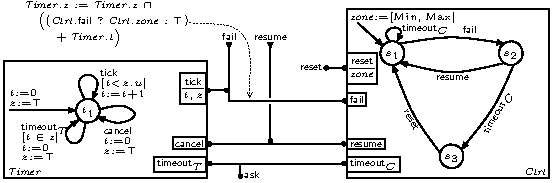
\includegraphics[width=0.9\columnwidth]{BIPspec-ArchFailureTimerMax-v4}
  \caption{The BIP specification of the Failure Monitor architecture}
  \label{fig:schema:ArchFailure:BIP}
\end{figure}

In this paper, we will use a running example, which is a refined
version of the Failure Monitor architecture
from~\cite{CubETH-case-study}.  Although \fig{schema:ArchFailure:BIP}
shows the full definition of this architecture, we will explain its
various elements progressively, as we define the corresponding
notions.

The model in \fig{schema:ArchFailure:BIP} has  components
%% The
%% component $\NameOprnd$ is an \emph{operand} of the architecture, \ie
%% it only has its interface defined: $(\emptyset, \{\PortFinish,
%% \PortResume, \PortFail\}, \export[\emptyset])$, with
%% $\export[\emptyset](p) = \emptyset$, for all $p \in \{\PortFinish,
%% \PortResume, \PortFail\}$.  
%% The other two components,
%
$\NameTimer$(imer) and $\NameCtrl$(ontrol), with interfaces
$\btuple{
  \{t, z\},
  \{\PortTick, \PortCancel, \PortTOT\},
  \bigl\{\PortTick \mapsto \{t, z\}\bigr\}
}$,
and
$\btuple{
  \{\mathit{zone}\},
  \{\PortReset, \PortFail, \PortResume, \PortTOC\},
  \bigl\{\PortFail \mapsto \{\mathit{zone}\}\bigr\}
}$, respectively.
%
%% \[
%% \begin{array}{@{}c@{\hspace{3mm}}c@{}}
%%   \bigl(
%%   \{t, z\},
%%   \{\PortTick, \PortCancel, \PortTOT\},
%%   \export[\NameTimer]
%%   \bigr)\,,
%%   %% \qquad
%%   &
%%   \bigl(
%%   \{\mathit{zone}\},
%%   \{\PortReset, \PortFail, \PortResume, \PortTOC\},
%%   \export[\NameCtrl]
%%   \bigr)\,,
%%   \\
%%   \export[\NameTimer](p) =
%%   \begin{cases}
%%     \{t, z\}, & \text{if } p = \PortTick,\\
%%     \emptyset, & \text{otherwise,}
%%   \end{cases}
%%   %% \]
%%   %% and
%%   %% \[
%%   %% \quad
%%   &
%%   \export[\NameCtrl](p) =
%%   \begin{cases}
%%     \{\mathit{zone}\}, & \text{if } p = \PortFail,\\
%%     \emptyset, & \text{otherwise.}
%%   \end{cases}
%% \end{array}
%% \]
%
%% , where $\export[\NameCtrl](\PortFail) =
%% \{\mathit{zone}\}$ and $\export[\NameCtrl](p) = \emptyset$, for all
%% other ports $p$; $\export[\NameTimer](\PortTick) = \{t, z\}$ and
%% $\export[\NameTimer](p) = \emptyset$, for all other ports $p$.
Variable $t$ is implicitly assumed to be an integer.  Variables $z$
and $\mathit{zone}$ are implicitly assumed to be integer intervals of
the form $[l,u]$.  For both types, we also implicitly assume the
natural ordering: increasing integers and interval inclusion.

%% are \emph{coordinators}\mdash they are specified
%% completely, including the states and transitions defining their
%% \emph{behaviour}.
Component \emph{behaviour} is defined by states %% ($\{\cstate{0},
%% \cstate{1}, \cstate{2}\}$, for $\NameCtrl$; $\{\tstate{0}\}$, for
%% $\NameTimer$)
and transitions.
The initial states
\tstate{0} and \cstate{0}, and valuations $\val{0}{\NameTimer} = \{t
\mapsto 0, z \mapsto \topinterval\}$ and $\val{0}{\NameCtrl} =
\{\mathit{zone} \mapsto [\mathrm{Min}, \mathrm{Max}]\}$ are shown by
the incoming arrows $\goesto{\TimerInit[]} \tstate{0}$ and
$\goesto{\IntervalInit[]} \cstate{0}$.\footnote{%
%
  We use $\topinterval$ to denote the top interval in the inclusion
  order, \ie $(-\infty, +\infty)$.
%
} The constants $\mathrm{Min}$ and $\mathrm{Max}$ are the parameters
of the architecture.

Transitions are labelled with ports of the
corresponding components, Boolean guards and update assignments on local
variables.  \Eg[,] the loop transition $\tstate{0}
\goesto{\PortTick, \GuardTick[], \TimerUpd[]} \tstate{0}$ in the
component $\NameTimer$ is labeled by the port $\PortTick$.  It can be
fired only when the current value of the local variable $t$ is less
than $z.u$.
%% , where $z = [l, u]$ is a local variable representing an
%% interval
Upon firing, this transition increments the value of $t$ by $1$.  The
guards and update assignments of the transitions of $\NameCtrl$ are
omitted.  The default values are the constant predicate $\true$ (true) and
the empty assignment {\noop}, respectively.  
%\noteLH{It looks like Max is in zone, I do not understand}
%
Clearly, all guards and update assignments are monotonic.

%% \todoSBin{Speak of guard monotonicity}

\begin{definition}[Component semantics]
  \label{defn:comp:semantics}
  The \emph{semantics} of a component $B = \tuple{Q, q^0, V,
  \val{0}{}, P, \export, \goesto{}}$ is %% given by
  the LTS denoted $\semopen{B} = \tuple{S,
  s^0, \goesto{}}$, where $S = Q \times \valuations{V}$, $s^0 =
  \tuple{q^0, \val{0}{}}$ and $\goesto{}$ is the minimal transition
  relation satisfying the rule
  %
  \begin{equation}
    \label{eq:comp:semantics}
    \infer{
      q \goesto{a, g, u} q'
      \and
      \val{}{} \models g
      \and
      \val[\primeit]{}{} = \tilde{\val{}{}}[u]
      \and
      \valdiff{\val{}{}}{\tilde{\val{}{}}} \subseteq \export(a)
    }{
      (q, \val{}{}) \goesto{a,\tilde{\val{}{}}} (q', \val[\primeit]{}{})
    }
    \,.
  \end{equation}
  %
  %% \todoSB{Do we actually need this?}\todoLH{I agree: I do not think we need this}
  %% \hl{The \emph{closed semantics} of $B$ is given by the LTS denoted
  %% $\semclosed{B} \bydef{=}\reachable{\semopen{B}}$, comprising
  %% only the reachable states of $\semopen{B}$.}
\end{definition}

The use of the intermediate valuation $\tilde{\val{}{}}$ in the
conclusion and the third premise of rule \eq{comp:semantics}
allows some of the variables to get new values before the
transition is actually fired.  Thus the component is \emph{open}
to the exchange of data with its environment.  However, the
fourth premise in \eq{comp:semantics} restricts the set of
variables, which can be affected by such data transfer, to those
that are exported through the ports participating in the
interaction.

\begin{definition}[Interaction model]
  \label{defn:im}
  For a finite set of component interfaces $(V_i, P_i,
  \export[i])^{i \in I}$, such that all $P_i$ and all $V_i$ are
  pairwise disjoint, %% \ie $\forall i \neq j,\ P_i \cap P_j = V_i \cap
  %% V_j = \emptyset$. 
  let $P = \bigcup_{i \in I} P_i$, $V = \bigcup_{i
    \in I} V_i$ and $\export : P \rightarrow 2^V$ such that, for any
  $p \in P_i$, $\export(p) = \export[i](p)$. 
%
  %% \noteSB{Updated this}\hl{and $V_a \bydef{=} \bigcup_{i \in
  %%   \supp{a}} \export[i](a \cap P_i)$ the set of component
  %% variables exported through $a$.}

  An \emph{interaction model over $(V, P, \export)$} is a set $\Gamma
  \subseteq 2^P \times \guards{V} \times \updates{V}$, such that,
  for any interaction $(a, g, u) \in \Gamma$, we have
  $g \in \guards{\export(a)}$ and $e \in \updates{\export(a)}$.\footnote{%
%
    Notice that this definition allows $(\emptyset, \true,
    \noop)$ and $(\emptyset, \false, \noop)$ to be included in
    $\Gamma$.
%
  }
  %% We call the set of ports $P$ the \emph{domain} of the
  %% interaction model.
\end{definition}

%% \noteLH{supp should go outside the definition}
When speaking of a set of components or interfaces, we will always
assume that it satisfies the disjointness assumption of \defn{im}.
%
We call the \emph{support} of a set of ports $a \subseteq P$, denoted
$\supp{a}$, either the set $\setdef{i \in I}{a \cap P_i \neq
  \emptyset}$ (for $P = \bigcup_{i=1}^n P_i$) or the set $\setdef{B
  \in \cB}{a \cap P_B \neq \emptyset}$ (for $P = \bigcup_{B \in \cB}
P_B$).  The precise meaning of this notation will always be clear from
the context.  Intuitively, for an interaction $(a, g, u)$, $\supp{a}$
denotes the set of the participating components.

\begin{definition}[Composition]
  \label{defn:im:sem}
  The \emph{composition} of a finite set of components $\cB = \tuple{Q_i,
  q^0_i, V_i, \val{0}{i}, P_i, \export[i], \goesto{}}^{i \in I}$ with
  the interaction model $\Gamma$ over $\tuple{V, P, \export}$ (as in \defn{im})
  is the component $\Gamma(\cB) = \tuple{Q, q^0, V, \val{0}{}, P,
    \export, \goesto{}}$, where
%
  $Q = \prod_{i \in I} Q_i$;
%
  $q^0 = (q_i^0)^{i \in I}$;
%
  $\val{0}{}: V \rightarrow \data$ is such that, for any $v \in
  V_i$, $\val{0}{}(v) = \val{0}{i}(v)$;
%
  and $\goesto{}$ is the minimal transition relation satisfying
  the rule
%
  \begin{gather*}
%%     \label{eq:im:empty}
%%     \infer{
%%       q_j \goesto{\emptyset, g, e} q_j'
%%       \and
%%       \forall i \neq j, q_i = q_i'
%%     }{
%%       (q_i)^{i \in I} \goesto{\emptyset, g, e} (q_i')^{i \in I}
%%     }\,,
%% %
%%     \\[0.5\baselineskip]
    \label{eq:im:sem}
%
    \infer{    
      (a, g, u) \in \Gamma
      \and
      a \neq \emptyset
      \and
      \forall i \in \supp{a}, q_i \goesto{a \cap P_i, g_i, u_i} q_i'
      \and
      \forall i \not\in \supp{a}, q_i = q_i'
%
      \\\\
      \textstyle
%
      g' = g \land \bigwedge_{i \in \supp{a}} g_i
      \and
      u' = u; u_i^{i \in \supp{a}}
    }{
      (q_i)^{i \in I} \goesto{a, g', u'} (q_i')^{i \in I}
    }\,.
  \end{gather*}
  %% \todoSBin{Add the intuitive explanation}
\end{definition}

\addSB{Intuitively, an interaction can be fired if all the involved
  components are ready to fire their corresponding transitions.  The
  other components do not change their states.  Both the interaction
  guard and those of the participating transitions must be satisfied.
  The update assignment of the interaction is executed first, followed
  by those of the components.}

Specifying interaction models as sets of sets of ports is not
practical due to their potentially exponential size.  An algebra of
connectors was introduced in \cite{BliSif08-acp-tc} in order to
structure interactions in BIP models.

Connectors are hierarchical, tree-like structures with component ports
at the leaves.  They define sets of interactions, based on the
attributes of the nodes, which may be either \emph{trigger}
(triangles in \fig{schema:ArchFailure:BIP}) or \emph{synchron}
(bullets in \fig{schema:ArchFailure:BIP}).
%
If all sub-connectors of a connector are synchrons, then an
interaction is allowed by the connector only if each subconnector
can contribute.
%
If at least one of the sub-connectors is a trigger, then any
interaction consisting of contributions of any set of sub-connectors
\emph{involving at least one of the triggers} is allowed.
%
The interaction model is defined as the set of all interactions
allowed by at least one of the connectors in the system.
%% The composition semantics of BIP systems consists in
%% firing exactly one interaction, enabled through at least one of the
%% top-level connectors, at each execution round.

For instance, the connector {\NameTimer.\PortTick
  \trigsynch (\PortFail \trigsynch \NameCtrl.\PortFail)} is a
two-level hierarchical connector.  In the second-level subconnector
{\PortFail \trigsynch \NameCtrl.\PortFail}, the port {\PortFail} is a
trigger, whereas {\NameCtrl.\PortFail} is a synchron.  Therefore, this
subconnector allows two interactions labelled $\{\PortFail\}$ and $\listset{\NameCtrl.\PortFail, \PortFail}$.  Similarly, at the top level,
{\NameTimer.\PortTick} is a trigger, whereas the second-level
subconnector is a synchron.  Hence, the overall connector allows the
interaction involving only one port {\NameTimer.\PortTick}\footnote{%
%
  Such interactions are called \emph{singleton interactions}.
%
} and any interaction involving both {\NameTimer.\PortTick} and
\emph{some} interaction of the second-level subconnector.  Combining
the two levels we can see that the entire connector defines the
following three interactions (observe that $\topinterval +
\NameTimer.t = \topinterval$ and $\NameTimer.z \cap \topinterval =
\NameTimer.z$):
%
\begin{gather*}
  \bigl(\{\NameTimer.\PortTick\},
  \true, \emptyset\bigr)
  %% \NameTimer.z := \NameTimer.z\bigr)
  ,
%
  \qquad
%
  \bigl(\{\PortFail, \NameTimer.\PortTick\},
  \true, \emptyset\bigr)
  %% \NameTimer.z := \NameTimer.z\bigr)
  ,
%
  \\
%
  \bigl(\{\NameCtrl.\PortFail, \PortFail, \NameTimer.\PortTick \},
  \true,
  \NameTimer.z := \NameTimer.z \cap (\NameCtrl.\mathit{zone} + \NameTimer.t)\bigr)
  .
\end{gather*}
%% \begin{align*}
%%   \bigl(\{\NameTimer.\PortTick\}&,
%%   \true, 
%%   \NameTimer.z := \NameTimer.z\bigr)
%%   \,,\\
%%   \bigl(\{\PortFail, \NameTimer.\PortTick\}&,
%%   \true,
%%   \NameTimer.z := \NameTimer.z\bigr)
%%   \,,\\
%%   \bigl(\{\NameCtrl.\PortFail, \PortFail, \NameTimer.\PortTick \}&,
%%   \true,
%%   \NameTimer.z := \NameTimer.z \cap (\NameCtrl.\mathit{zone} + \NameTimer.t)\bigr)
%%   \,.
%% \end{align*}

%% \todoSB{Update this}
%% \hl{For instance, in \fig{schema:ArchFailure:BIP}, the two ports
%% $\NameTimer.\PortStart$ and $\NameCtrl.\PortFail$ are always
%% synchronised, since they belong to exactly one binary sub-connector,
%% where they are both synchrons.  In particular, this means that
%% whenever the transition \cstate{0} \goesto{\PortFail} \cstate{1} is
%% fired, so is the transition \tstate{0} \goesto{\PortStart,
%%   \TimerInit[]} \tstate{1}, initialising the timer.  The binary
%% connector $\NameTimer.\PortStart \twosynch
%% \NameCtrl.\PortFail$ is a sub-connector of a hierarchical connector,
%% where the port $\NameOprnd.\PortFail$ is a trigger.  Thus, the above
%% interaction can only happen together with $\NameOprnd.\PortFail$,
%% forming a ternary interaction.  On the contrary, being a trigger, the
%% port $\NameOprnd.\PortFail$ can fire alone, forming a singleton
%% interaction.}

%% \todoSBin{Speak of data transfer}

%% \todoSBin{Provide the interaction model}

\begin{definition}[Priority model]
  \label{defn:priority}
  A \emph{priority model} over a component interface $(V, P,
  \export)$\footnote{%
%
    Notice that the export function $\export$ has no impact on the
    priority model definition.
%
  } is a strict partial order on interactions: $\pi
  \subseteq \bigl(2^P \times \guards{V} \times \updates{V} \bigr)^2$.

  We write $\alpha \prec_\pi \beta$, for $(\alpha, \beta) \in \pi$, and 
   $\filter{\alpha} \bydef{=} \bsetdef{\beta \in (2^P \times
    \guards{V} \times \updates{V})}{\alpha \prec_\pi \beta}$, for the set of
  interactions that have higher priority than $\alpha$.
\end{definition}

\begin{definition}[Application of priority]
  \label{defn:priority:sem}
  The application of a priority model $\pi$ over $(V, P, \export)$
  to a component $B = \tuple{Q, q^0, V, \val{0}{}, P, \export, \goesto{}}$
  is the component $\pi(B) = \tuple{Q, q^0, V, \val{0}{}, P, \export,
  \goesto[\pi]{}}$, where $\goesto[\pi]{}$ is the minimal transition
  relation satisfying the rule (we denote
  $\filter[q]{\alpha} \bydef{=} %% \filter{\alpha} \cap
  %% \bsetdef{\beta \in (2^P \times \guards{V} \times \updates{V})}
  \setdef{\beta \in \filter{\alpha}}{q \goesto{\beta}}$)
%
  \begin{equation*}
    \label{eq:priority:sem}
%
    \infer{
      \alpha = (a, g, u)
      \and
      q \goesto{a, g, u} q'
      \and
      \textstyle
      g' = g \land \bigwedge_{(b, h, w) \in \filter[q]{\alpha}} \lnot h
    }{
      q \goesto[\pi]{a, g', u} q'
    }\,.
  \end{equation*}
%
  %% \todoSBin{Add the intuitive explanation}
\end{definition}

\addSB{Intuitively, an interaction can be fired only if all the
higher-priority interactions available in the current state are
disabled by their respective guards.}

In this paper, we will only consider the so-called \emph{maximal
  progress} priority $\mu$, where $(a, g, u) \prec_\mu (b, h, w)$ iff $a
\varsubsetneq b$ (\ie $a \subseteq b$ and $a \neq b$).  In
\secn{conclusion}, we discuss the possibility of generalising the
obtained results to other priority models.
%
Below, we will assume that the maximal progress priority $\mu$ is
applied after each composition with an interaction model.

%% Finally, \emph{priorities}\mdash defined by a strict partial order on
%% the set of possible interactions\mdash narrow the choice among the
%% enabled interactions at any given round.  The default priority is the
%% so-called \emph{maximal progress}, whereby among any two interactions
%% $a \subset b$ (as sets of ports), $b$ has higher priority than $a$.
In our running example, under the maximal progress priority, the
port $\NameTimer.\PortTick$ will never fire alone in a global state,
where the \noteSB{This turns out to be the first use of the word. I am tempted to pretend I did not notice.}\hl{dangling} port $\PortFail$ is also enabled. 

%% Adding priorities $\NameOprnd.\PortFinish < \NameCtrl.\PortReset$ and
%% $\NameOprnd.\PortFinish < \NameOprnd.\PortResume$, ensures that, after
%% a failure, the operation performed by $\NameOprnd$ cannot finish
%% unless it is explicitly resumed or the system is reset.

%% \begin{note}
%%   \label{rem:maxprogress}
%% \end{note}


%% %****************************************************************
%% \subsection{Running example: Failure Monitor architecture}
%% \label{secn:failure-monitor}

%\noteLH{Ludo ou simon: essayer de remonter la description generique en debut de section}

%****************************************************************
\subsubsection{Architectures}
\label{secn:archi}

Architectures are partially defined BIP models, where \emph{dangling}
ports serve as placeholders for the eventual connection with
additional \emph{operand} components.

%% Contrary to standard BIP models, architectures comprise one or several
%% \emph{operand} components, whereof only the set of \emph{ports} is
%% given.  Here, the operand component is $\NameOprnd$ and its interface
%% consists of the ports $\PortFinish$, $\PortResume$ and $\PortFail$.

%% Application of the Failure Monitor architecture ensures that, whenever
%% a failure is registered in the operand component, the system will be
%% reset, unless a resumption is registered within $\mathrm{Max}$ time
%% units (more details in Sect.~\ref{section:resultOA}).

%% \noteLHin{should we say that always epsilon C is the epsilon of C?}

\begin{definition}[Architecture]
  \label{defn:arch}
  An \emph{architecture} is a tuple $A = \tuple{\cC, V_A, P_A,
    \export[A], \Gamma}$, where
%  
  \begin{itemize}
\item
  $\cC$ is a finite set of \emph{coordinating components},
  %% with pairwise disjoint sets of ports and variables,
  such that
  $\bigcup_{C \in \cC} P_C \subseteq P_A$ and
  $\bigcup_{C \in \cC} V_C \subseteq V_A$;
%
  ports in $P_A \setminus \bigcup_{C \in \cC} P_C$, which do not
  belong to any of the coordinating components are called
  \emph{dangling};

\item
  $\export[A] : P_A \rightarrow 2^{V_A}$ is an export function, such
  that $\export[A](p) = \export[C](p)$, for any $C \in \cC$ and $p \in
  P_C$ and $\export[A](p) \subseteq V_A \setminus \bigcup_{C \in \cC}
  V_C$ for any dangling port $p$; and

\item
  $\Gamma \subseteq 2^{P_A} \times \guards{V_A} \times \updates{V_A}$
  is an interaction model over $(V_A, P_A, \export[A])$.
  \end{itemize}

\end{definition}

\begin{definition}[Application of an architecture]
  \label{defn:arch:application}
  Let $A = \tuple{\cC, V_A, P_A, \export[A], \Gamma}$ be an architecture and let $\cB$
  be a set of components, such that
  $V_A \subseteq V \bydef{=} \bigcup_{B \in \cB \cup \cC} V_B$,
  $P_A \subseteq P \bydef{=} \bigcup_{B \in \cB \cup \cC} P_B$
%
  %% \begin{align}
  %%   \bigcup_{B \in \cB} V_B \cap \bigcup_{C \in \cC} V_C = \emptyset\,,
  %%   &&
  %%   V_A \subseteq V \bydef{=} \bigcup_{B \in \cB \cup \cC} V_B\,,
  %%   \\
  %%   \bigcup_{B \in \cB} P_B \cap \bigcup_{C \in \cC} P_C = \emptyset\,,
  %%   &&
  %%   P_A \subseteq P \bydef{=} \bigcup_{B \in \cB \cup \cC} P_B\,,
  %% \end{align}
%
  and $\export[A](p) = V_A \cap \export[B](p)$, for any $B \in \cB$
  and $p \in P_A \cap P_B$.
%
  The \emph{application of the architecture $A$ to the set of
  components $\cB$} is the component $ A(\cB) \bydef{=}
  \mu\bigl((\IMextend{\Gamma}{P})(\cC \cup \cB)\bigr)$, where
%
  $\IMextend{\Gamma}{P} \bydef{=}
  \bsetdef{
    (a, g, u)
  }{
    a \subseteq P,
    (a \cap P_A, g, u) \in \Gamma
  }$
  is
  %% is the \emph{extension} of the interaction
  %% model $\Gamma$ to the set of ports $P$, \ie
  the interaction model
  over $(V, P, \export)$, with
  \[
  \export(p) = 
  \begin{cases}
    \export[C](p), & \text{for all } C \in \cC, p \in P_C,
    \\
    \export[B](p), & \text{for all } B \in \cB, p \in P_B,
  \end{cases}
  \]
%% defined by \noteLH{looks like this also depends on Pa}
%% %
%%   \noteSB{It does, indeed.  To be completely rigorous, I could replace
%%     this with something like $\Gamma\uparrow_{P_A}^P$ but this is
%%     quite heavy and the dependency is already implicit from the fact
%%     that $\Gamma$ is defined on $P_A$}
%% %
%%   \noteSB{Which one of \eq{im:extension} and \eq{im:extension1} is
%%     more intuitive?}
%
  %% \begin{align}
  %%   \label{eq:im:extension}
  %%   \IMextend{\Gamma}{P} &\bydef{=}
  %%   \bsetdef{
  %%     (a \cup a', g, e)
  %%   }{
  %%     (a, g, e) \in \Gamma, a' \subseteq P \setminus P_A
  %%   }
  %%   \\
  %%   \label{eq:im:extension1}
  %%   &= 
  %%   \bsetdef{
  %%     (a, g, e)
  %%   }{
  %%     a \subseteq P,
  %%     (a \cap P_A, g, e) \in \Gamma
  %%   }
  %% \end{align}
%
  and $\mu$ is the maximal progress priority model.
\end{definition}

%% \todoSBin{Define equivalence $\arequiv$?}

An architecture $A$ enforces coordination constraints on the
components in $\cB$.  The interface $(V_A, P_A, \export[A])$ of an
architecture $A$ contains all ports of the coordinating
components $\cC$ and the dangling ports, which must belong to
the components in $\cB$.  In the application $A(\cB)$, the ports
belonging to $P_A$ can only participate in the interactions
defined by the interaction model $\Gamma$ of $A$.  Ports which do
not belong to $P_A$ are not restricted and can participate in any
interaction.  %% In particular, they can join the interactions in
%% $\Gamma$ (see \eq{im:extension}).  If the interface of the
%% architecture covers all ports of the system, \ie $P = P_A$, we
%% have $P\setminus P_A = \emptyset$ and the only interactions
%% allowed in $A(\cB)$ are those belonging to $\Gamma$.  Notice also
%% that the restrictions imposed by \defn{arch:application} on the
%% set of operand components $\cB$ ensure that an interaction in
%% $\IMextend{\Gamma}{P}$ can only refer to variables of the
%% participating components.
%
%% Finally, 
The definition of $\IMextend{\Gamma}{P}$ requires that
an interaction from $\Gamma$ be involved in every interaction
belonging to $\IMextend{\Gamma}{P}$.  To allow the ports from $P
\setminus P_A$ to be fired independently in $A(\cB)$, one must
have $(\emptyset, \true, \noop) \in \Gamma$.  

In our running example, there are four dangling ports.  Intuitively, the
architecture monitors the activation of the dangling port {\PortFail}, then
waits for a period comprised between $\mathrm{Min}$ and $\mathrm{Max}$
and, unless {\PortResume} is activated, asks for a system reset
through an invocation of the dangling port {\PortAsk}.

\begin{definition}[Composition of architectures]
  \label{defn:arch:composition}
  Let $A_i = \tuple{\cC_i, V_{A_i}, P_{A_i}, \export[A_i], \Gamma_i}$, for $i = 1,2$,
  be two architectures.  The \emph{composition} of $A_1$ and
  $A_2$ is the architecture $A_1 \arcomp A_2 = \tuple{\cC_1 \cup \cC_2,
  V_{A_1} \cup V_{A_2}, P_{A_1} \cup P_{A_2}, \export[A_1] \cup \export[A_2], \Gamma}$, where
%
  \begin{equation}
    \label{eq:arch:composition}
    \Gamma = \bsetdef{
      (a, g^1 \land g^2, u^1 \expmix u^2) 
    }{
      (a \cap P_{A_i}, g^i, u^i) \in \Gamma_i,
      \text{ for } i = 1,2
    }
    \,.
  \end{equation}
\end{definition}

\begin{proposition}[Properties of $\arcomp$]
  \label{prop:arcomp:nice}
  %% Architecture composition
  $\arcomp$ is associative and commutative.
  %%; it is idempotent if all coordinating components
  %% are deterministic; $A_{id} = \bigl(\emptyset, \emptyset,
  %% \emptyset, \emptyset, \{(\emptyset, \true, \noop)\}\bigr)$ is its neutral element, \ie for
  %% any architecture $A$, we have $A \oplus A_{id} \arequiv A$.
  %% Furthermore, for any component $B$, we have $A_{id}(B) = \mu(B)$.
\end{proposition}
%
\begin{proof}[Sketch of the proof]
  %% Commutativity and associativity 
  Follows from the corresponding
  properties of set union, Boolean conjunction and
  semilattice meet.
%
%% \todoLH{Check when equivalence is defined}
%%   Suppose we have two architectures $A \arequiv A'$.  This does not
%%   necessarily mean that their sets of coordinating components
%%   coincide.  However, if all the involved coordinating components
%%   are deterministic, then, in any state of $(A \arcomp A')(\cB)$,
%%   both architectures will impose the same restrictions, enabling
%%   the same interactions between the coordinating and operand
%%   components.  Hence, we have $(A \arcomp A')(\cB) = A(\cB) =
%%   A'(\cB)$.  Since this holds for any set of components $\cB$, we
%%   conclude that $A \arcomp A' \arequiv A \arequiv A'$.
%% %
%%   The properties of $A_{id}$ follow immediately from the
%%   definitions of architecture application and composition.
\end{proof}

%% The last statement of \prop{arcomp:nice} highlights a subtle point:
%% $A_{id}$ is the neutral element of the $\arcomp$ operator\mdash it is
%% not the identity operator on components.

%****************************************************************
\subsubsection{Preservation of safety properties}
\label{secn:safety}

For a component $B$, we denote $S_{\semopen{B}}$,
$s^0_{\semopen{B}}$ the corresponding constituents of
$\semopen{B}$.

\begin{definition}[Properties]
  \label{defn:property}
  Let $B$ be a component.  A \emph{(safety) property} 
  of $B$ is a predicate $\Phi$ on
  $S_{\semopen{B}}$, such that $\bigl((q,
  \val{}{}) \models \Phi\bigr) \land (\val[\primeit]{}{} \order
  \val{}{})$ implies $(q, \val[\primeit]{}{}) \models \Phi$.
  %% ,
  %% where we write $(q, \val{}{}) \models \Phi$ iff $\Phi(q,
  %% \val{}{}) = \true$.
  A property $\Phi$ is \emph{initial} if
  $s^0_{\semopen{B}} \models \Phi$.
  %% \todoSB{Do we need this?}\hl{;
  %% it is \emph{reachable} iff there exists a possibly empty path
  %% $s^0_{\semopen{B}} \goesto{a^1, \val{1}{}} s^1 \goesto{a^2,
  %%   \val{2}{}} \cdots \goesto{a^n, \val{n}{}} s^n$, such that
  %% $s^n \models \Phi$}.
\end{definition}

\addSB{Although we define properties as state predicates, any
  appropriate logic can be used to specify them.  For instance, the
  property \emph{``There is always a possibility to reset the system
    after a failure''} enforced by the Failure Monitor architecture
  can be specified using CTL as $\AG (\PortFail \rightarrow \EF
  \PortReset)$.  Additional properties are provided in \app{properties}.}

%% \todoSB{Cite the original paper somewhere.}
The main idea of our approach is that an architecture enforces
its characteristic property on the set of its operand components.
From this point of view, the set of coordinating components is
not relevant, neither are their states.  Thus, to talk about
properties enforced by architectures, we consider properties on
the unrestricted composition of the operand components as
formalized by the following definition.

\begin{definition}[Enforcing properties]
  \label{defn:enforce}
  Let $A = \tuple{\cC, P_A, V_A, \export[A], \Gamma}$ be an architecture; let $\cB$
  be a set of components and $\Phi$ an initial property of
  their parallel composition $\Gamma_{\|}(\cB)$,
  with $\Gamma_{\|} = \setdef{(a,\true,\emptyset)}{a \subseteq \bigcup_{B \in \cB} P_B}$.
  We say that \emph{$A$ enforces $\Phi$ on
    $\cB$} iff, for every state $s = (s_c, s_b)$ reachable in
  $\semopen{A(\cB)}$, with 
  $s_c \in \prod_{C \in \cC} S_{\semopen{C}}$ and
  $s_b \in \prod_{B \in \cB} S_{\semopen{B}}$,
  we have $s_b \models \Phi$.
\end{definition}

According to the above definition, when we say that an
architecture enforces some property $\Phi$, it is implicitly
assumed that $\Phi$ is initial for the coordinated components.
Below, we omit mentioning this explicitly.

\defn{up:compat} in \secn{arch:appendix} provides a formal definition
of the notion of \emph{upwards compatibility}, which we present here
informally due to page limitations.  Two architectures $A_1$ and $A_2$
are said to be upwards compatible iff, whenever their composition
involves the fusion of two interactions $a_1 = a \cap P_{A_1}$ and
$a_2 = a \cap P_{A_2}$ (see \eq{arch:composition}), whereof one, say
$a_1$, is inhibited in a given state by a larger interaction $b_1
\supset a_1$, there exists an interaction $b_2 \supseteq a_2$ that can
be fused with $b_1$ to form an interaction enabled in the same state.

\begin{theorem}[Preserving enforced properties]
  \label{thm:combining}
  Let $\cB$ be a set of components; let $A_i = \tuple{\cC_i, V_{A_i},
  P_{A_i}, \export[A_i], \Gamma_i}$, for $i = 1,2$, be two upwards compatible architectures
  enforcing on $\cB$ the properties $\Phi_1$ and $\Phi_2$
  respectively.  The composition $A_1 \arcomp A_2$ enforces on
  $\cB$ the property $\Phi_1 \land \Phi_2$.
\end{theorem}

%****************************************************************
%****************************************************************

\subsection{Open pNets}
\label{secn:pNets}
This section briefly describes pNets, see~\cite{HMZ-FORTE2016} for more complete   description.
pNets are tree-like structures, where the leaves are either
\emph{parameterised labelled transition systems (pLTSs)}, expressing the
behaviour of basic processes, or \emph{holes}, used as placeholders
for unknown processes.
Nodes of the tree are synchronising artefacts using a
set of \emph{synchronisation vectors} that express the possible
synchronisation between the parameterised actions of a subset of the
sub-trees.

\paragraph{pNets definition.}
\label{section:pNets}
A pLTS is a labelled transition system with variables that can be
used to characterise a state, as part of actions, guards, and
assignments. 
%Without loss of generality and to simplify the formalisation, we suppose 
%here that 
%variables are local to each 
%state: each state has its set of variables disjoint from the others. Transmitting 
%variable values from one state to the other can be done by explicit assignment. 
%Similarly, to simplify the management of variables and without loss of expressivity, we 
%suppose that transitions looping to the same state does not do assignments.
%Note that we make no assumption on the finiteness of the set of states, nor
%on the finite branching of the transition relation.
We  define the set of actions a pLTS can use ($a$
ranges over action labels):\\
%. Action terms are  of the form 
$\alpha=a(?x_i^{i \in I}, 
\Expr_j^{j \in J})$, where $?x_i^{i \in I}$ are input variables, $\Expr_j^{j \in J}$ 
are expressions.

\begin{definition}[pLTS]
\label{pLTS}
A pLTS is a tuple
$\pLTS\triangleq\mylangle S,s_0, \to\myrangle$ where:
\begin{itemize}
\item
$S$ is a set of states, $\vars(s)$ denotes the set of associated variables;
\item
$s_0 \in S$ is the initial state;
%\item[$\bullet$]
 %Variables in
%$\iv(\alpha)$ are assigned by the action, other variables can be assigned
%by the additional assignments.
\item $\to \subseteq S \times L \times S$ is the transition relation and 
$L$ is the set of labels of the form
% SB: I removed a new paragraph here, ok?
$\langle \alpha,~g,~u\rangle$,
where $\alpha$ is a parameterised action, $\alpha \in\actions{\variables}$; 
$g\in\boolexprs{\variables}$ is a guard over variables of the source state and the 
action, and $u\in\assigns{\variables}$
assigns updated value for variables in the destination state. 
%%% SHORTEN BY LUDO
%If 
%$s \xrightarrow{\langle \alpha,~g,~u\rangle} s'\in \to $ then 
%% REMOVED BECAUSE USELESS: $\iv(\alpha)\!\subseteq\! \vars(s')$, 
%		$\vars(\alpha)\backslash \iv(\alpha)\!\subseteq\! \vars(s)$, 
%		$\vars(g)\!\subseteq\! \vars(s)\cup\vars(\alpha)$, and
%		$\vars(\codom(u))\!\subseteq\! \vars(s)\cup\vars(\alpha)\land 
%		\vars(\dom(u))\!\in\!\vars(s')$. %,  and $s= s'\Rightarrow J=\emptyset$. 
%\noteLH{is dom and codom clear?}
%\noteSB{Not sure: I understand, because I know what is meant, but this is not a canonical use, so should be explained. Will be solved if we roll back to \mbox{$(?x_i := e_i)^{i \in I}$} or \mbox{$\overline{?x := e}$}.}
%\noteLH{COORDINATION: I believe we should remove the constraints}		
\end{itemize}
\end{definition}
%Now we define
%pNets as constructors for hierarchical behavioural structures.
A pNet composes several pNets, pLTSs, and holes playing the role of process parameters.
A  pNet  exposes
 global actions resulting from the synchronisation of internal actions in some sub-pNets. 
This synchronisation  is specified by  \emph{synchronisation vectors}.
Actions involved in the synchronisation vectors do
not need to distinguish input variables, \ie they 
have the form $a(\Expr_j^{j \in J})$.


\begin{definition}[pNets]\label{defn:pnets}
A pNet is a hierarchical structure where leaves are pLTSs and holes: %\footnote{Typing can 
%be added to pNets by defining and checking their interfaces, called 
%sort~\cite{HMZ-FORTE2016}}:
$\pNet\triangleq \pLTS~|~\mylangle \pNet_i^{i\in I}, J, \symb{SV}_k^{k\in 
K}\myrangle$
where
\begin{itemize}
\item $\pNet_i^{i\in I}$ is the family of sub-pNets;
%  $\pNet_i^{i\in I}$ is a family of sub-pNets where $I\in\I_\P$ is the set over which 
%sub-pNets are indexed.

\item $J$ is a set of indexes, called \emph{holes}.
$I$ and $J$ are \emph{disjoint}: $I\!\cap\! J=\emptyset$,  $I\!\cup\! J\neq\emptyset$
%\item[$\bullet$] $\Sort_j \subseteq \AlgAS$ is a set of action terms, denoting the 
%\emph{sort} of
%hole $j$.

\item $\symb{SV}_k^{k\in K}$ is a set of
  synchronisation vectors. % (\hl{$K\in\I_\P$}). 
$\forall k\!\in\! K,
  \symb{SV}_k\!=\SV{\!\alpha_{l}^{l\in I_k \uplus J_k}}{\alpha'_k}{g_k}$, where
  $\alpha'_k\in \actions{\variables}$, $I_k\subseteq I$, $J_k\subseteq J$, and 
  $\vars(\alpha'_k)\subseteq \bigcup_{l\in I_k\uplus 
  J_k}{\vars({\alpha_l})}$. The global action of a vector $\symb{SV}_k$ is
$\alpha'_k$. The Boolean expression $g_k $, such that $\vars(g_k)\subseteq \bigcup_{l\in 
I_k\uplus J_k}{\vars({\alpha_l})}$, is a guard associated to the vector.


\end{itemize}
%We define the set of holes and leaves of a pNet as follows:
%  \begin{itemize}
%\item
The set of \emph{holes} $\Holes(\pNet_{i_1})$ of a pNet is the indexes of the holes of the pNet 
itself plus the indexes of all the holes of its subnets (we suppose those indexes 
disjoints). A pNet $Q$ is \emph{closed} if it has no hole: $\Holes(Q)=\emptyset$; else it
is said to be \emph{open}.
%
%defined inductively; the sets of holes
%in a pNet node and its subnets are all disjoint:
%  \[\begin{array}{l}
%\Holes(\mylangle S,s_0, \to\myrangle) \!=\! \emptyset \\
%\Holes(\mylangle \pNet_i^{i\in I}\!,\Sort_j^{j\in J}\!, \overline{\symb{SV}}\myrangle) 
%=J\uplus{\displaystyle \bigcup_{i\in 
%I}\Holes(\pNet_i)}\\
%\forall i\in I.\, \Holes(\pNet_i)\cap J=\emptyset\\
%\forall i_1,i_2\in I.\,i_1\neq i_2\Rightarrow  
%\Holes(\pNet_{i_1})\cap\Holes(\pNet_{i_2})=\emptyset
%\end{array}\]
%\item
The set of \emph{leaves} of a pNet is the set of all pLTSs occurring in the structure, as an 
indexed family of the form $\Leaves(\pNet)= \mylangle \pNet_i \myrangle^{i \in L}$.
%\end{itemize}

\end{definition}






\paragraph{Operational Semantics for Open pNets.}
\label{section:op-semantics}

\noteLH{a pred is a g a post is a u (modified macros!)}
\renewcommand{\Pred}{g}
\renewcommand{\Post}{u}
The semantics of an open pNets is expressed as an open automaton, i.e., an automaton where each transition composes the actions of several holes, 
the transition occurs if some predicates hold, and can involve a 
 state modifications.
%\TODO{adopt a uniform notation for open transitions, almost each instance has a 
%different 
%notation! I suggest p,l,pr,po using \{\} for p,l,po as they are sets}
\begin{definition}[Open transition]
	\label{defn:OpenTransitions}
	An \emph{open transition} over a
	set $J$ of holes  and a set of states $\mathcal{S}$ is 
	a structure of the form:
\\[-2ex]	
	\begin{mathpar}
	\inferrule*[myfraction=\reddottedrule]
	{	\beta_j^{j\in J}, \Pred, \Post}
	{s \OTarrow {{\alpha}}s'}
	\end{mathpar}
	Where $s, s'\in\mathcal{S}$ and $\beta_j\in\actions{\variables}$
        is an action of the hole $j$. $v$ is a variable denoting the resulting action
        of this open transition. \Pred\ is a predicate 
	over the different variables of the
	terms, labels, and states  $\beta_j$, $s$, $\alpha$. $\Post\in 
	\assigns{\variables}$\ is 
	a set of assignments that are the effects of the transition.
Open transitions are identified modulo logical equivalence on their predicate.
\end{definition}
%\begin{definition}[Open transitions]
%	\label{def:OpenTransitions}
%	An \emph{open transition} over a set \noteSB{In the architecture section, I say that 
%we omit indices on $\goesto{}$ and that they are always clear from the 
%context.}\hl{$(S_i,s_{0 i}, \rightarrow_i)^{i\in
%	I}$} of LTSs, a
%	set $J$ of holes with sorts $\Sort_j^{j\in J}$, and a set of states $\mathcal{S}$ is 
%	a structure of the form:	
%	\begin{mathpar}
%	\inferrule*[myfraction=\reddottedrule]
%	{\{s_i~{\xrightarrow{a_i}}_i ~s_i^{\prime}\}^{i\in I},
%		\{\xrightarrow{b_j}_j\}^{j\in J}, \Pred, \Post}
%	{s \OTarrow {v}s'}
%	\end{mathpar}
%	Where $s, s'\in\mathcal{S}$ and for all
%        $i\in I$, $s_i{\xrightarrow{a_i}}_i s_i^{\prime}$ is a transition of the
%	LTS $(S_i,s_{0 i}, \rightarrow_i)$, and \noteSB{Why insist on ``transition'' and 
%$\goesto{b_j}_j$? Why not simply ``$b_j$ is an action in the sort 
%$\Sort_j$?}\hl{$\xrightarrow{b_j}_j$
%        is a transition of the hole $j$}, for any action $b_j$ in the
%        sort $\Sort_j$.  
%        of this open transition. \Pred\ is a predicate 
%	over the different variables of the
%	terms, labels, and states $s_i$, $b_j$, $s$, $v$. \Post\ is a set of equations that 
%	hold \emph{after the open transition}, they are represented as a substitution of the 
%	form $\{x_k\gets \Expr_k\}^{k\in K}$ \noteLH{considering the level of abstraction I 
%	would like to just put $\Post_=e$}
%	where $x_k$ are variables of $s'$, $s'_i$, and $e_k$ are expressions over the other 
%	variables of the open transition.
%\end{definition}



The red dotted rule expresses an implication but at a different logical level compared to  a normal 
inference rule. 
 The open transition is  a logical implication that uses a simple logic with the 
 expressive power  given by the predicate algebra (it must include logical 
 propositions and equality). We differentiate classical (black) inference rules that use 
 an expressive (higher order) logic and are paper rules from open transition rules that use a simpler  logic,  define automata transitions, and could  be handled 
 mechanically.


\begin{definition}[Open automaton]
	\label{defn:open-automaton}
	An \emph{open automaton} is a structure\\ $A =
	<J,\mathcal{S},s_0,\mathcal{T}>$ where:
	\begin{itemize}
		\item   $J$ is a  set of indices,
		\item   $\mathcal{S}$ is a set of states and $s_0$ an initial state
		among $\mathcal{S}$,
		\item $\mathcal{T}$ is a set of open transitions and for each
		$t\in \mathcal{T}$ there exist  $J'$ with  $J'
		\subseteq J$, such that $t$ is an open transition over  $J'$,
		and  $\mathcal{S}$.
		
	\end{itemize}
\end{definition}
	

%
%Then the semantics of a pNet is characterized by a set of {\em open
%transitions}, where the hypotheses on process parameters are
%replaced by 1) transitions of the pLTSs at the leaves, and 2) formal
%hypotheses on the transitions of the holes. A {\em predicate} is used
%to relate the parameters and names appearing in the actions of the
%leaves and the holes involved in the rules, but also appearing in  the resulting action.


We build the semantics of open pNets as an open automaton where  the states are
tuples of states of the pLTSs at the leaves. We denote them $\triangleleft\ldots\triangleright$ for distinguishing tuple 
states from other tuples. given by 
Definition~\ref{def-states}. 
The open transitions first
 project the global state into states of the leaves, then apply
pLTS transitions on these states, and compose them with the sort of the holes according to the synchronisation defined in the synchronisation vectors. More precisely, each open transition between two states is defined as a composition of transition from some pLTSs and actions of some holes as follows: 1) the actions of the holes involved in the transition, 2) a guard  built from the synchronisation vectors coordinating the holes and the transitions involved; 3) assignments defined by the pLTSs transitions involved. The synchronisation vectors also define the global action. The global state evolution is also defined by the set of state transitions of the pLTSs involved in the pLTSs.



\begin{example}\emph{An open-transition.}
  \label{OT:enable-composed}
  The \texttt{Failure TimerMonitor} pNet of \Fig{FailureTimer:pNet} has 2 controllers 
  and 2 holes. One of its possible open-transitions is:\\[-2ex]
%%   \footnote{Note the underlined action notation that we use to represent synchronised actions, i.e. actions that are the result of a synchronisation and that we declare as \emph{non-observable}. Those actions are only used for monitoring purposes and statement of properties but cannot be synchronised again in a synchronisation vector. This allows us to define a weak bisimilarity equivalence with p=compositional properties.}
%%   : 
%% \noteLH{underline notation might be a bit too much for this paper : see at the end if we remove it or not (will we use it?)}
% \smallskip
%$  OT_1  = \openrule
%{\emptyset, \{t:=0, z:=TopInt, zone:=[minZone,maxZone]\} }
%{\ostate{00} \OTarrow{\underline{\alpha_4}} \ostate{11}}
%$
%\medskip
\begin{small}\[ \openrule
  {\{B\mapsto fail(b0)\},\\
    t<GetMax(z) \land b1=true \land b1=>b0 \land z1= (z \cap (b1?zone;TopInt)+t),
    \{z:=z1\} }
  {\ostate{11} \OTarrow{\alpha_0} \ostate{12}}
  \]
\end{small}\vspace{-1.5ex}
%
%The first one, $OT_1$, corresponds to the simultaneous initialisation
%of both controlers. No hole is active at that time, and the resulting
%global action is denoted $\alpha_4$.

It correspond to the firing of the connector
$''tick, fail, fail''$. It states that, if the hole B performs an action $fail$, and the (complex) guard is satisfied, then the variable $z$ is set to $z1$ (as specified by the guard), then the transition below the dotted line occurs and a global action labelled $\alpha_0$ occurs. Only the second pLTS performs a transition from state $1$ to state $2$.
The guard corresponds both to the guard of this transition and to synchronisation vector constraints.
\end{example}
%
%\begin{definition}[States of open pNets]\label{def-states}
%  A state of an open pNet is a tuple (not necessarily finite) of the
%  states of its leaves.
%
%  For any pNet p, let $\Leaves(p) = \mylangle S_i,{s_i}_0, \to_i\myrangle^{i \in L}$ be 
%  the set of pLTS at its leaves,
%  then $States(p) = \{\triangleleft s_i^{i\in L}
%  \triangleright| \forall i\in L. s_i \in S_i\}$.
%A pLTS being its own single leave:
%  $States(\mylangle S,s_0, \to\myrangle) = \{\triangleleft s \triangleright| s \in S\}$.
%
%The initial state is defined as:
%$InitState(p) = \triangleleft {{s_i}_0}^{i\in L}  \triangleright$.
%\end{definition}
%
%
%
%%% \begin{example} \emph{State of a pNet}
%%%   The states of pNet \texttt{EnableCompL} are:
%%%   $\triangleleft 00 \triangleright, \triangleleft 10 \triangleright, \triangleleft 11 
%%%\triangleright$
%%% \end{example}
%
%\paragraph{Predicates:}
%Let
%$\mylangle\overline{\pNet},\overline{\Sort},\overline{\symb{SV}}\myrangle$
%be a pNet. Consider a synchronisation vector $\symb{SV}\in \overline{\symb{SV}}$. We 
%define a
%predicate $\Pred$ relating
%the actions of the involved sub-pNets and the resulting actions. This predicate verifies:
%\begin{multline}
%\Predsv(\SV{{(\alpha'_i)}^{i\in I}, {(\beta'_j)}^{j\in J}} 
%{\alpha'} {g}, \alpha_i^{i\in I}, \beta_j^{j\in J}, \alpha)\Leftrightarrow \\
%\forall i\in I.\, \alpha_i=\alpha'_i\land \forall j \in J.\, \beta_j=\beta'_j \land 
%\alpha=\alpha' 
%\land g
%\end{multline}
%
%
% 
%
%Somehow, this predicate entails a verification of satisfiability in the sense that if the 
%predicate $\Pred_{\symb{sv}}$ is not satisfiable, then the transition associated with the 
%synchronisation will not occur in the considered state. 
%
%
%In any other case (if the action families do not match or if there is no valuation of
%variables such that the above formula can be ensured) the predicate is undefined.
%
%This definition is not constructive but it is easy to build the predicate constructively
%by brute-force unification of the sub-pNets
%actions with the corresponding vector actions, possibly followed by a simplification
%step.
%
%
%
%
%\begin{definition}[Operational semantics of open pNets]
%	\label{defn:operationalSemantics}
%	The semantics of a pNet $p$ is an open automaton $A = 
%	<Holes(p),States(p),InitState(p),
%	\mathcal{T}>$ where $\mathcal{T}$ is the smallest set of open transitions		
%	satisfying the rules below:
%%	\begin{itemize}
%%		\item $J$ is the set of holes: $Holes(p)= J$. 
%		%  \item $\overline{L}^L = Leaves(p), \overline{H}^J = Holes(p)$
%%		\item ${\mathcal{S}} = States(p)$ and $s_0 = InitState(p)$
%%		\item $\mathcal{T}$ is the smallest set of open transitions		satisfying the 
%%rules below:
%%	\end{itemize}
%	
%	%% \TODO{ We should be careful here: after (re) reading "Huimin
%	%% 	Lin, 'Symbolic Transition Systems with Assignements', Concur'96" I
%	%% 	think handling assignments is not trivial, even for comparisons of pLTSs. }
%
%
%	
%	The rule for a pLTS  checks that the guard 
%	is verified and transforms assignments into post-conditions:
%	
%	\begin{description}
%		\item[{\bf Tr1:}]
%	$\inferrule
%		{ s \xrightarrow{\langle \alpha,~g,~u\rangle} s'\in \to  }
%		{ \mylangle  S,s_0, \to \myrangle
%			\models
%			\openrule
%			{\emptyset ,
%			g,u}
%			{\ostate{s} \OTarrow{\alpha} \ostate{s'}}
%		}
%		$
%	\end{description}
%%	Note that this note is greatly simplified by the fact that variables are local to 
%%	thread; introducing global state variables or accepting loops to the same 
%%	state would 
%%	require to reason 
%%	on the scope of 
%%	each variables, and to introduce additional variables to handle the several occurence 
%%	of the same pLTS variable in the predicates. Indeed the constraints on pLTS 
%%	transitions 
%%	ensure that the same variable never appears both on the left and on the right of the 
%%	equations of a predicate.
%	
%	The second rule deals with pNet nodes: for each possible
%	synchronisation vector (of index $k$) applicable to the rule subject, the premisses
%	include one {\em open transition} for each sub-pNet involved , one possible
%	{\em action} for each Hole involved, and the predicate relating these
%	with the resulting action of the vector. The sub-pNets involved are split between two 
%	sets, $I_2$ for subnets that are pLTSs, and $I_1$ for the others, $J$ is the set of 
%	holes involved in the transition\footnote{Formally, if $SV_k \!=\! \SV{\alpha_m^{m 
%	\in M}}{\alpha'}{g}$ is a synchronisation vector  of \pNet\  then $J=M\cap 
%	\Holes(\pNet)$, $I_2=M\cap \Leaves(\pNet)$,  $I_1=M\setminus J \setminus 
%	I_2$}.                                                                    
%	           
%	                                                       
%	\begin{description}
%		\item[{\bf Tr2:}]
%	\end{description}
%	
%%	\noindent
%%\begin{mathpar}
%%    \mprset {vskip=1ex}
%%\inferrule
%%    {
%%\Leaves(\mylangle \overline{\pNet}, \overline{\Sort}, \symb{SV}_k^{k\in 
%%    	K}\myrangle) \!=\! \pLTS_l^{l\in L} \qquad  	
%%k\!\in\! K \qquad SV_k \!=\! \SV{(\alpha'_m)^{m \in I_1\uplus I_2\uplus J}}{\alpha'}{g} 
%%\\
%%\\     	
%%	\forall m\!\!\in\!\! I_1. {\pNet_m 
%%	\models\openrule
%%    	{
%%    	\beta_{j}^{j\in J_m}, \Pred_m, \Post_m}
%%    	{\ostate{s_{i}^{i \in L_m}} \OTarrow {\alpha_m}
%%    		\ostate{(s_i^\prime)^{i\in L_m}}} }	
%%  \qquad
%%\forall m\!\!\in\!\! I_2.		{ \pNet_m 
%%    	 \models
%%    	\openrule
%%    	{\emptyset, \Pred_m, \Post_m}
%%    	{\ostate{s_m} \OTarrow {\alpha_m}
%%    		\ostate{s_m'}} }\\\\
%%     J' = \biguplus_{m\in I_1}\!\! J_m \uplus J 	\\
%%    	\Pred = \bigwedge_{m\in (I_1\uplus I_2)}\!\! \Pred_m \land
%%    	\Pred_{\symb{sv}}(SV_k,\alpha_m^{m\in (I_1\uplus I_2)},\beta_j^{j\in J},\alpha)\\ 
%%    		I' = \biguplus_{m\in I_1}\!\! I_m \uplus I_2
%%    	\\\forall i\in	L\backslash I'.\,s'_i=s_i \\
%%    \fresh(\alpha'_m,\alpha',\beta_j,\alpha) 
%%    }
%%    {\mylangle \overline{\pNet}, \overline{\Sort}, \symb{SV}_k^{k\in K}\myrangle
%%    	\models
%%    	{\openrule
%%    		{
%%    		{\beta_j}^{j\in J^\prime}, \Pred, \uplus_{m\in I_1\uplus I_2} 
%%    		\Post_m}
%%    		{\ostate{s_i^{i\in L}} \OTarrow {\alpha}
%%    			\ostate{(s_i^\prime)^{i\in L}}}
%%    	}
%%    }
%%\end{mathpar}  
%	\noindent
%\begin{mathpar}
%    \mprset {vskip=.8ex}
%\inferrule
%    {
%\Leaves(\mylangle {\pNet}_m^{m\in I}, \set{\Sort}, \symb{SV}_k^{k\in 
%    	K}\myrangle) \!=\! \pLTS_l^{l\in L} \qquad  	
%k\!\in\! K \qquad SV_k \!=\! \SV{(\alpha'_m)^{m \in I_1\uplus I_2\uplus J}}{\alpha'}{e_b} 
%\\
%\\     	
%	\forall m\!\!\in\!\! I_1. {\pNet_m 
%	\models\openrule
%    	{
%    	\beta_{j}^{j\in J_m}, \Pred_m, \Post_m}
%    	{\ostate{s_{i}^{i \in L_m}} \OTarrow {\alpha_m}
%    		\ostate{(s_i^\prime)^{i\in L_m}}} }	
%  \qquad
%\forall m\!\!\in\!\! I_2.		{ \pNet_m 
%    	 \models
%    	\openrule
%    	{\emptyset, \Pred_m, \Post_m}
%    	{\ostate{s_m} \OTarrow {\alpha_m}
%    		\ostate{s_m'}} }\\\\
%     J' = \biguplus_{m\in I_1}\!\! J_m \uplus J 	\\
%    	\Pred = \bigwedge_{m\in I_1\uplus I_2}\!\! \Pred_m \land
%    	\Predsv(SV_k,\alpha_m^{m\in I_1\uplus I_2},\beta_j^{j\in J},\alpha)\\ 
%    	\forall i\in	L\backslash \left(\biguplus_{m\in I_1}\!\! L_m \uplus I_2\right).\,s'_i=s_i \\
%    \fresh(\alpha'_m,\alpha',\beta_j,\alpha) 
%    }
%    {\mylangle {\pNet}_m^{m\in I}, \set{\Sort}, \symb{SV}_k^{k\in K}\myrangle
%    	\models
%    	{\openrule
%    		{
%    		{\beta_j}^{j\in J^\prime}, \Pred,  \biguplus_{m\in I_1\uplus I_2} 
%    		\Post_m}
%    		{\ostate{s_i^{i\in L}} \OTarrow {\alpha}
%    			\ostate{(s_i^\prime)^{i\in L}}}
%    	}
%    }
%\end{mathpar}        

pNets have already been used to define a behavioural semantics for distributed components~\cite{AmeurBoulifa2017}, in these works, from a pNet model with finite instantiations of parameters, correctness properties can be verified by model-checking. 
More recently, a bisimulation theory with composition properties have been formalised for open pNets~\cite{HMZ-FORTE2016}, and a SMT framework has been developed  for verifying properties of parametrised open pNets.

%\todoLHin{add a paragraph about pnets properties and usage, here are a few points (to be completed and written up properly depending on what we need}
%
%- pnets as a model for gcm components (behaviour, distributed systems, verification)
%
%- used for finite model checking (with finite domains for parameters)
%
%- smt framework for reasoning on infinite models
%
%- a theory of pnets: composition properties , stong (and weak) bisim
%	** extract a few useful composition theorems? **


%OLD	\begin{description}
%		\item[{\bf Tr2:}]\noteSB{I do not understand why the second line $pNet_m 
%\models\dots$ is not subsumed by the first one?}
%	\end{description}
%	
%	\noindent
%    $\inferrule
%    {k\!\in\! K \\SV_k \!=\! \alpha_m^{m \in I\uplus J} \!\to\! 
%    \alpha' |g \\
%    	Leaves(\mylangle \pNet_i^{i\in I'}, \overline{\Sort}, \symb{SV}_k^{k\in 
%    	K}\myrangle) \!=\! \pLTS_l^{l\in L} \\    	
%    	\forall m\!\!\in\!\! I. 	
%    {\left(\begin{array}{l}
%	{\pNet_m \models\inferrule*[myfraction=\reddottedrule]
%    	{\{s_{i}\xrightarrow{a_{i}}_i s_{i}'\}^{i\in I_m^\prime},
%    	\{\xrightarrow{b_{j}}_j\}^{j\in J'_m}, \Pred_m, \Post_m}
%    	{\ostate{s_{i}^{i \in L_m}} \OTarrow {v_m}
%    		\ostate{(s_i^\prime)^{i\in L_m}}}\lor }\\
%		{ \pNet_m 
%    	 \models
%    	\inferrule*[myfraction=\reddottedrule]
%    	{\{s_m \xrightarrow{v_m} s_m'\},\emptyset, \Pred_m, \Post_m}
%    	{\ostate{s_m} \OTarrow {v_m}
%    		\ostate{s_m'}} \land I'_m=\{m\} \land J'_m=\emptyset}
%\end{array}\right)}\\
%    	%\land
%    	%Leaves(\pNet_m) = \overline{\pLTS}^{L_k})  	
%     J' = \biguplus_{m\in I}\!\! J'_m \uplus J 	\\
%    	\Pred = \bigwedge_{m\in I}\!\! \Pred_m \land
%    	\Pred_{\symb{sv}}(SV_k,v_m^{m\in I},b_j^{j\in J},v)\\ 
%    		I' = \biguplus_{m\in I}\!\! I_m'
%    	\\\forall i\in	L\backslash I'.\,s'_i=s_i \\
%    {\tt fresh}(\alpha_m,\alpha',b_j,v) 
%    }
%    {\mylangle \pNet_i^{i\in I'}, \overline{\Sort}, \symb{SV}_k^{k\in K}\myrangle
%    	\models
%    	{\inferrule*[myfraction=\reddottedrule]
%    		{\{s_i\xrightarrow{a_i}_i s_i^{\prime}\}^{i\in I^\prime},
%    		\{\xrightarrow{b_j}_j\}^{j\in J^\prime}, \Pred, \uplus_{m\in I_k} 
%    		\Post_m}
%    		{\ostate{s_i^{i\in L}} \OTarrow {v}
%    			\ostate{(s_i^\prime)^{i\in L}}}
%    	}
%    }
%    $
%        \TODO{may be explain how $\Pred(SV,a_i^{i\in I_k},b_j^{j\in
%            J_k},v)$ is built ? You mean more than what is written on previous page????}
	%%    \TODO{I have tentatively added the sort constraint on hole actions, that was
	%%not included in the first version... I'm unsure whether this is the best place to
	%%include it, because it may change the decidability conditions on predicates}
	


%****************************************************************
%****************************************************************

\section{Encoding of architectures into open pNets}
\label{secn:encoding}

We will define the encoding of BIP architectures into pNets by
associating to each architecture $A = \tuple{\cC, V_A, P_A,
  \export[A], \Gamma}$ with $C = \tuple{Q_C, q^0_C, V_C, \val{0}{C},
  P_C, \export[C], \goesto{}}$, for each $C \in \cC$, \emph{and a
  partition $\partition \subseteq 2^{P_A}$ of its dangling ports} (\ie
$\biguplus_{D \in \partition} D = P_A \setminus \bigcup_{C \in \cC}
P_C$), the corresponding pNet $\nopri[A, \partition]$.
%
%% and $D_1 \cap D_2 = \emptyset$, for any two distinct $D_1, D_2
%% \in \partition$.
%
%% Notice that this addition 
%% is a matter of convenience, since one can
%% use the trivial partition $\partition \bydef{=} \{P_A \setminus \bigcup_{C
%%   \in \cC} P_C\}$.

Below, for the sake of clarity, we start by presenting in
\secn{enc:nopri} the encoding of $A$ into pNets without accounting for
any priority model (see \secn{components}).  Then, in
\secn{enc:maxprog}, we slightly modify this encoding to include the
implicitly assumed maximal progress priority.

%****************************************************************
\subsection{Encoding without the priority model}
\label{secn:enc:nopri}

Recall that $\Gamma$ is an interaction model over the interface
$\tuple{V_A, P_A, \export[A]}$, \ie these interface elements are
implicitly involved in the definition of $\Gamma$.
%
We define $\nopri[A, \partition] \bydef{=} \pNetTuple{(\nopri[C])^{C
    \in \cC}, \partition, \nopri[\Gamma]}$, where $\nopri[C]$ and
$\nopri[\Gamma]$ are the encodings of a coordinator $C$ and the
interaction model $\Gamma$ respectively.

\paragraph{Encoding the coordinators}
To encode a coordinator $C$, we 1)~introduce a fresh initial state with an additional
$\init$ transition that initialises all the variables to those defined
by the initial valuation $\val{0}{C}$ of $C$, 2)~define a pNet action algebra that associates, as action parameter, an
additional Boolean value to each port, 3)~create pNet transitions that reflect the original transitions of
$C$ with $\true$ as parameter and 4)~create additional loop transitions marked by
$\false$.

Formally,  $\nopri[C] \bydef{=} \pNetTuple{S, s_0, \goesto[{\nopri[C]}]{}}$, such that
%
\begin{itemize}
\item $s_0 \not\in Q_C$ is fresh and $S = Q_C \cup \{s_0\}$,
\item $\vars(s) = V_C$, for all $s \in Q_C$, and $\vars(s_0) =
  \emptyset$,
%% \item the transition relation $\goesto[{\nopri[C]}]{}$ is defined as
%%   the union of three sets of transitions
%%   (with $\mathit{init} \bydef{=} \bigl(x := \val{0}{C}(x)\bigr)^{x \in V_C}$):
%% %
%%   \begin{multline}
%%     \label{eq:nopri:trans}
%%     {\goesto[{\nopri[C]}]{}} \bydef{=}
%%     \bsetdef{\tuple{s, a(\true), g, u, s'}}{
%%       \tuple{s, a, g, u, s'} \in \goesto{}}
%%     \\    
%%     \cup
%%     \bsetdef{\tuple{s, a(\false), \true, \noop, s}}{
%%       s \in Q_C, a \in P_C}
%%     %% \\
%%     \cup
%%     \bigl\{(s_0, \init, \true, \mathit{init}, q^0_C)\bigr\}
%%     \,.
%%   \end{multline}

\item ${\goesto[{\nopri[C]}]{}} \bydef{=} T_1 \cup T_2 \cup T_3$, with
  $T_1 = \bsetdef{\tuple{s, a(\true), g, u, s'}}{
      \tuple{s, a, g, u, s'} \in \goesto{}}$,
  $T_2 = \bsetdef{\tuple{s, a(\false), \true, \noop, s}}{
      s \in Q_C, a \in P_C}$,
  $T_3 = \bigl\{(s_0, \init, \true, \mathit{init}, q^0_C)\bigr\}$
    and $\mathit{init} \bydef{=} \bigl(x := \val{0}{C}(x)\bigr)^{x \in V_C}$.
\end{itemize}

The loop transitions marked by $\false$ will be used in the encoding
of connectors.  Each BIP connector can define several interactions,
\ie ports involved in a connector need not necessarily always
participate.  On the contrary, each action in a pNet synchronisation
vector must participate in the synchronisation.  To address this
difference, we use the classical~\cite{milner83-calculi} approach,
whereby non-participation of a port in an interaction is simulated
by an additional loop transition.

\Fig{FailureTimer:pNet} shows the encoding of the Failure Monitor
architecture, including the encodings of the two coordinators, \ie
$\nopri[\NameTimer]$ and $\nopri[\NameCtrl]$.  Notice that the
encoding in the figure is slightly optimised: some of the ports do not
have an associated Boolean value, nor the additional loop transitions.
\todoSB{Revise this if necessary}\hl{We will explicitate this optimisation after we define the
encoding of the interaction model.}

\begin{figure}[t]
  \centering
  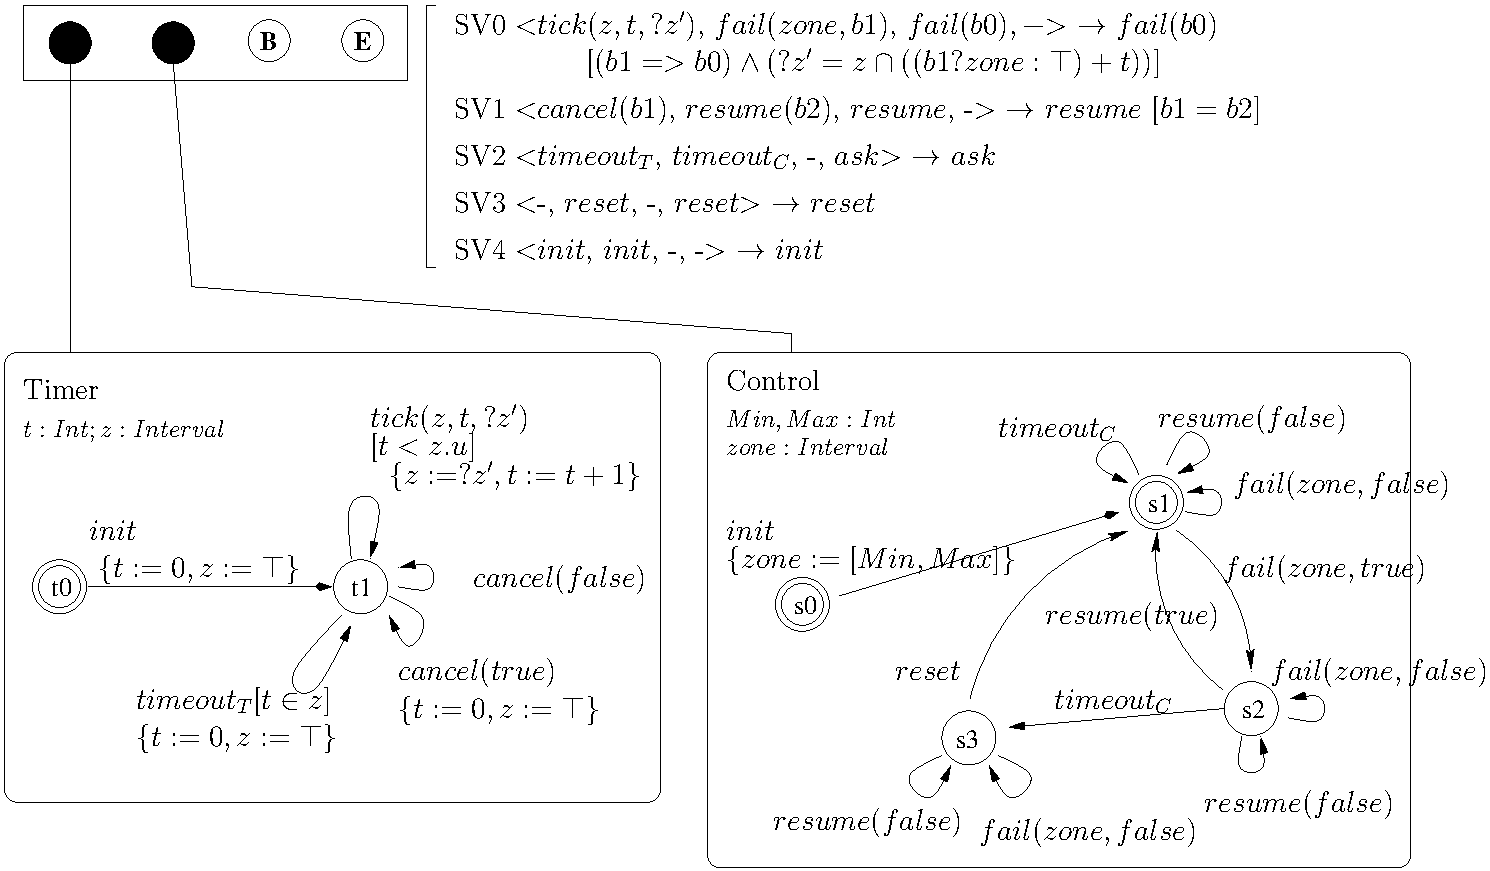
\includegraphics[width=0.9\columnwidth]{FailureTimerPNET-v4}
  \caption{The open pNET encoding the Failure Monitor architecture (\fig{schema:ArchFailure:BIP}) without the priority model}
  \label{fig:FailureTimer:pNet}
\end{figure}

%% \begin{figure*}[t]
%%   \fbox{%
%%   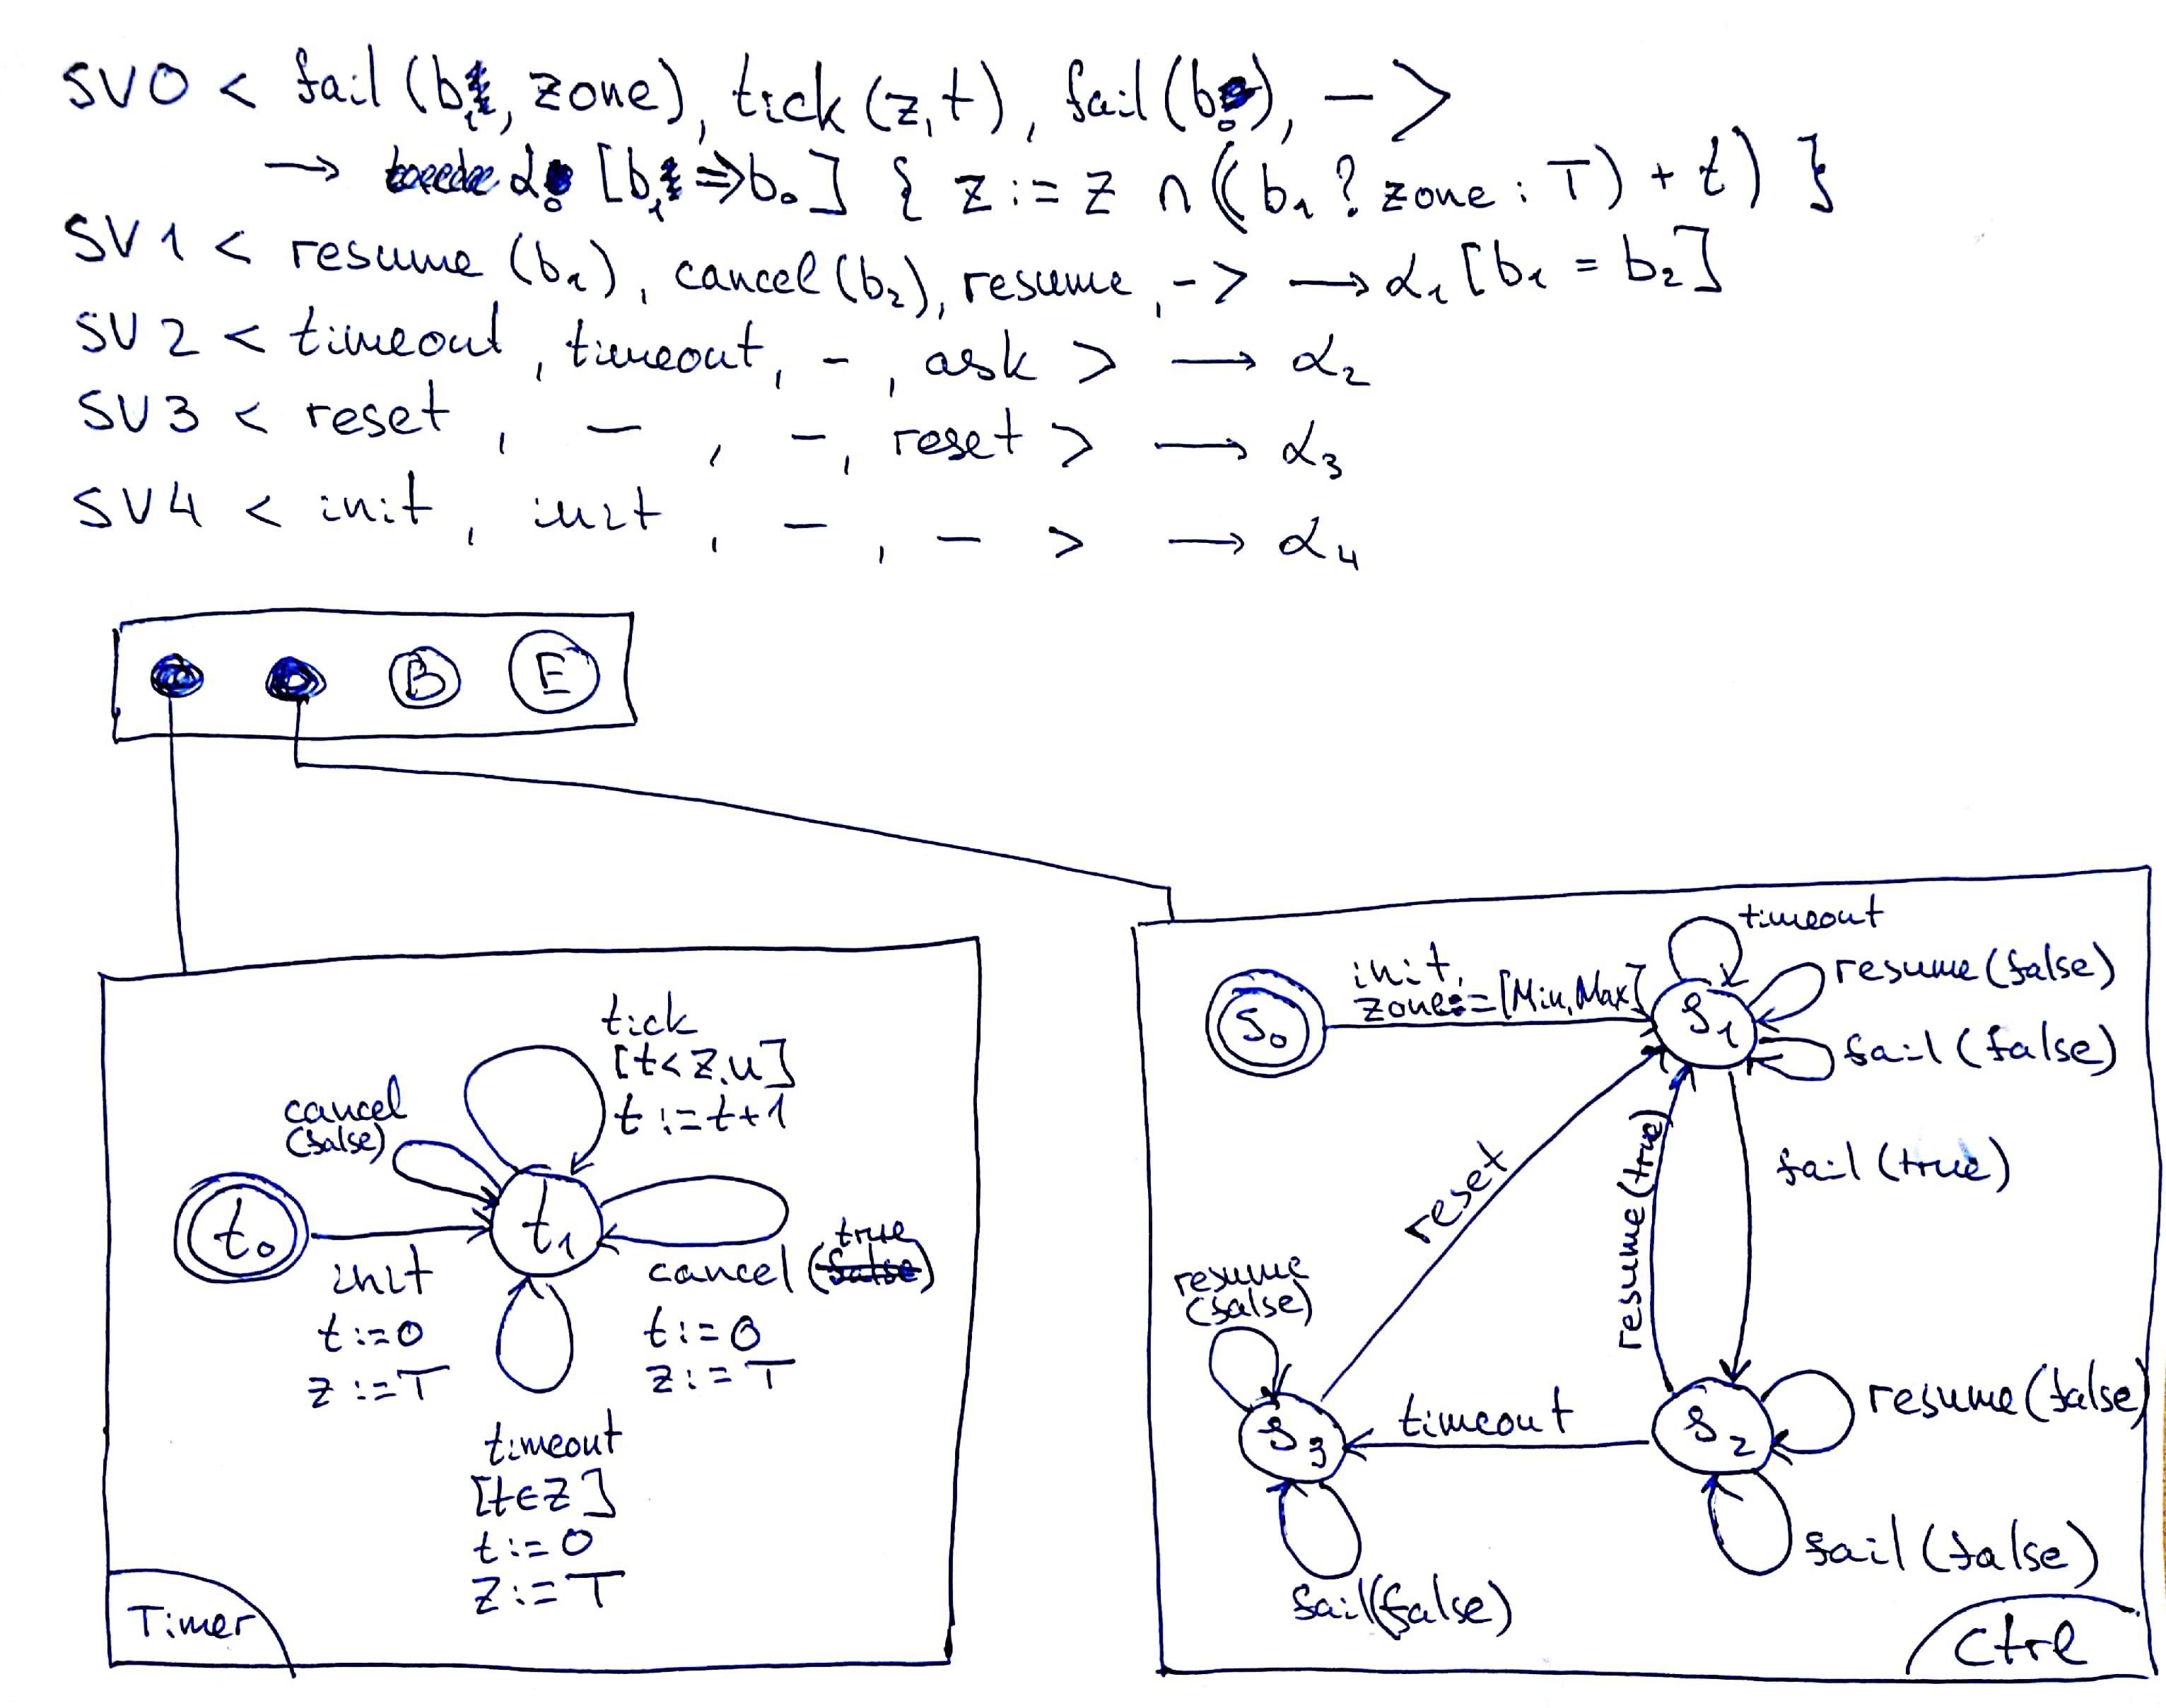
\includegraphics[width=\textwidth]{BIPspec-ArchFailureTimerMax-v4-no-pri}}
%%   \caption{Encoding of the Failure Monitor architecture
%%     (\fig{schema:ArchFailure:BIP}) as an open pNet (without the
%%     priority model) \hl{\bf (Error in the picture: First two positions in the synchronisation vectors must be transposed)}}
%%   \label{fig:enc:nopri}
%% \end{figure*}

\paragraph{Encoding the interaction model}
%% First of all, recall that $\nopri[A, \partition ] \bydef{=}
%% \pNetTuple{(\nopri[C])^{C \in \cC}, \partition, \nopri[\Gamma]}$.
%% Thus, 
The holes in $\nopri[A, \partition]$ are indexed by the elements of
the partition \partition.  For the encoding of our running example, we
take $\partition = \bigl\{\{\PortFail, \PortResume\},\{\PortAsk,
\PortReset\}\bigr\}$.  This corresponds to the intuition that the
dangling ports {\PortFail} and {\PortResume} will be provided by a 
monitored component, whereas {\PortAsk} and {\PortReset} correspond to
the actions provided by the ``environment'' (other components of the
system) that are invoked in case of a persistent failure.  As for
the encoding of the coordinators, in the synchronisation vectors of
\nopri[\Gamma], we will associate Boolean values to the actions
corresponding to these ports.

The encoding of the interaction model is based on its representation
as a set of connectors. \noteSB{%
%
  A legitimate question is whether we actually need to do this,
  instead of listing explicitly the individual interactions, then
  associating a synchronisation vector to each one of them?  One of
  the factors is the encoding pNets$\rightarrow$SAT: is it better to
  have more or fewer SVs if the price is additional Boolean variables?
  The other factor might be the facility of maximal progress
  encoding\mdash TBC.  Traceability.  Anything else?
%
} Indeed, as illustrated by the Failure Monitor architecture in
\fig{schema:ArchFailure:BIP}, each connector can define several
allowed interactions, depending on its hierarchical structure and the
use of synchrons and triggers.

In order to encode these interactions using only one synchronisation vector, we use
the additional Boolean values associated to each port by the encoding
of coordinator components.  We observe that the three ports in this
connector form a ``causality chain'': {\NameCtrl.\PortFail} can only
participate in the interaction if the dangling port {\PortFail}
participates, which in turn can only participate if
{\NameTimer.\PortTick} does so.  These dependencies can be rewritten
as Boolean implications $\NameCtrl.\PortFail \Rightarrow \PortFail$
and $\PortFail \Rightarrow \NameTimer.\PortTick$.
%
The conjunction of these two implications can be used as a guard for
the synchronisation vector encoding connector {\NameTimer.\PortTick
  \trigsynch (\PortFail \trigsynch \NameCtrl.\PortFail)}.

However, notice
that, within the scope of this connector, {\NameTimer.\PortTick}
participates in all the interactions.
%
Furthermore, {\NameTimer.\PortTick} is not involved in any other
connector.  Therefore, the loop transition in \nopri[\NameTimer]
labelled by $\PortTick(\false)$ can never be taken and, therefore can
be removed from the encoding.  Furthermore, since only the transition
labelled by $\PortTick(\true)$ is ever taken, 
%
the
implication $\PortFail \Rightarrow \NameTimer.\PortTick$ is a tautology and can also be discarded.

We obtain the
synchronisation vector SV0 shown in \fig{FailureTimer:pNet}, where $b_0$ and
$b_1$ are the Boolean values associated to the actions encoding the
ports {\PortFail} and {\NameCtrl.\PortFail}, $\alpha_0$ is a fresh
action name.  The guard $b_1 \Rightarrow b_0$ encodes the causal
relation among ports {\NameCtrl.\PortFail} and {\PortFail}.  Notice
that, in our encoding, all three ports are present in the
synchronisation vector.  \Fig{FailureTimer:pNet} shows
the four synchronisation vectors SV0\ndash SV3 corresponding to the
connectors in \fig{schema:ArchFailure:BIP} and an additional vector
SV4, synchronising the {\init} transitions of the two pLTSs.

The general case encoding relies on the causal semantics of the
algebra of BIP connectors \cite{BliSif10-causal-fmsd}.  Disregarding
the variables and data transfer, the Algebra of Connectors $\ac(P)$
\cite{BliSif07-acp-emsoft} provides a syntactic notation for the BIP
connectors.  The causal semantics of the connectors, given in terms of
the Algebra of Causal Interaction Trees $\ct(P)$, explicitates the
causal dependencies discussed above, through an encoding mapping
$\tau: \ac(P) \rightarrow \ct(P)$.  Another mapping $R: \ct(P)
\rightarrow \cru(P)$ encodes causal interaction trees into systems of
causal rules, which are Boolean implications similar to the ones in
the example above.  We briefly summarise the key definitions and
results in \app{algebras}.  The $\ac(P)$, $\ct(P)$ and $\cru(P)$
representations of the connectors in \fig{schema:ArchFailure:BIP} are
shown in \tab{connectors}.

\begin{table}[t]
  \caption{Algebraic representations of the connectors in \fig{schema:ArchFailure:BIP} (see \app{algebras})}
  \label{tab:connectors}
  \resizebox{\columnwidth}{!}{%
  \begin{tabular}{@{}c|c|c@{}}
    \hline {\bf Connector} & {\bf Causal Interaction Tree} & {\bf
      System of Causal Rules}
    \\\hline    
%
    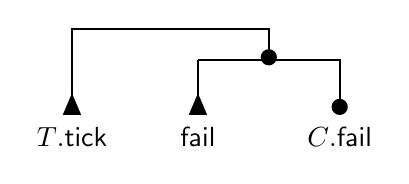
\begin{tikzpicture}[shorten >=1pt,node distance=.7cm,>=stealth']

      \node(caa) {}; % node distance=5cm [right of=start]
      \node[node distance=1cm] (cb) [below of=caa]{\PortFail};
      \node[node distance=1.8cm] (cc) [right of=cb]{\NameCtrl.\PortFail};
      \node[node distance=1.6cm] (ca) [left of=cb]{\NameTimer.\PortTick};

      \draw [style=-*, thick, black] ($(caa.south)+(0,.1cm)$) -- ++(right:.5cm) -| (cc.north);
      \draw [style=-triangle 45 reversed, thick, black]  ($(caa.south)+(0,.1cm)$) -| (cb.north);
      \draw [style=-*, thick, black] ($(caa.south)+(0,.5cm)$) -- ++(right:.2cm) -| ($(caa.south)+(+.9,0cm)$);
      \draw [style=-triangle 45 reversed, thick, black]  ($(caa.south)+(0,.5cm)$) -| (ca.north);
    \end{tikzpicture}
%
    &
%
    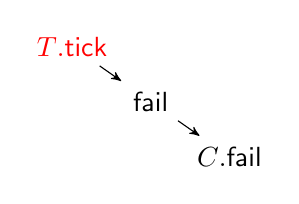
\begin{tikzpicture}[shorten >=1pt,node distance=.7cm,>=stealth'
        ,initial text=
        ,every state/.style={draw=black,thick}
        ,group/.style = {draw=black,thin,rectangle, minimum width=2.5cm}
        ,port/.style = {font=\small, minimum size=5mm}
        ,legend/.style = {font=\bf}
      ]

      \node(tick){\color{red}\NameTimer.\PortTick};
      \node[node distance=1cm](x) [right of=tick]{};
      \node(fail) [below of=x] {\PortFail};
      \node[node distance=1cm](y) [right of=fail]{};      
      \node(ctrlfail) [below of=y] {\NameCtrl.\PortFail};
      
      \draw[style=->] (tick) -> (fail);
      \draw[style=->] (fail) -> (ctrlfail);
    \end{tikzpicture}
%
    &
%
    $
    \begin{aligned}[b]
      \NameCtrl.\PortFail &\Rightarrow
      \PortFail {\color{red}{}\land \NameTimer.\PortTick}
      \\
      {\color{red}\PortFail} &{\color{red}{}\Rightarrow \NameTimer.\PortTick}
      \\
      {\color{red}\NameTimer.\PortTick} &{\color{red}{}\Rightarrow \true}
      \\
      {\color{red}\true} &{\color{red}{}\Rightarrow \NameTimer.\PortTick}

    \end{aligned}
    $
%
    \\\hline
%
    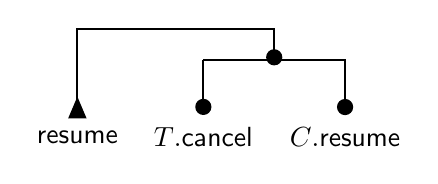
\begin{tikzpicture}[shorten >=1pt,node distance=.7cm,>=stealth']

      \node[](baa) {}; % node distance=1.8cm [right of=start]
      \node[node distance=1cm] (bb) [below of=baa]{\NameTimer.\PortCancel};
      \node[node distance=1.8cm] (bc) [right of=bb]{\NameCtrl.\PortResume};
      \node[node distance=1.6cm] (ba) [left of=bb]{\PortResume};


      \draw [style=-*, thick, black] ($(baa.south)+(0,.1cm)$) -- ++(right:.5cm) -| (bc.north);
      \draw [style=-*, thick, black]  ($(baa.south)+(0,.1cm)$) -| (bb.north);
      \draw [style=-*, thick, black] ($(baa.south)+(0,.5cm)$) -- ++(right:.2cm) -| ($(baa.south)+(+.9,0cm)$);
      \draw [style=-triangle 45 reversed, thick, black]  ($(baa.south)+(0,.5cm)$) -| (ba.north);
    \end{tikzpicture}
%
    &
%
    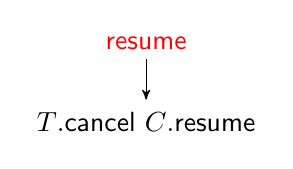
\begin{tikzpicture}[shorten >=1pt,node distance=.7cm,>=stealth'
        ,initial text=
        ,every state/.style={draw=black,thick}
        ,group/.style = {draw=black,thin,rectangle, minimum width=2.5cm}
        ,port/.style = {font=\small, minimum size=5mm}
        ,legend/.style = {font=\bf}
      ]

      \node(res){\color{red}\PortResume};
      \node[node distance=1cm](rest) [below of=res] {\NameTimer.\PortCancel\ \NameCtrl.\PortResume};
      \draw[style=->] (res) -> (rest);
    \end{tikzpicture}
%
    &
%
    $
    \begin{aligned}[b]
      \NameCtrl.\PortResume &\Rightarrow
      {\color{red}\PortResume \land{}} \NameTimer.\PortCancel
      \\
      \NameTimer.\PortCancel &\Rightarrow 
      {\color{red}\PortResume \land{}} \NameCtrl.\PortResume
      \\
      {\color{red}\PortResume} &{\color{red}{}\Rightarrow \true}
      \\
      {\color{red}\true} &{\color{red}{}\Rightarrow \PortResume}
    \end{aligned}
    $
%
    \\\hline
%
    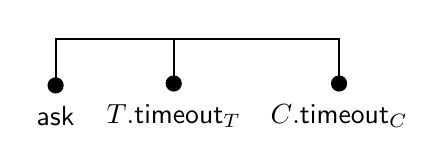
\begin{tikzpicture}[shorten >=1pt,node distance=.7cm,>=stealth']

      \node (start) {};
      \node(h4)[left of=start]{}; %, node distance=1.5cm

      \node[node distance=1cm] (ab) [below of=start] {\NameTimer.\PortTOT};
      \node[node distance=2.1cm] (ac) [right of=ab]{\NameCtrl.\PortTOC};
      \node[node distance=1.5cm] (aa) [left of=ab]{\PortAsk};

      \draw [style=-*, thick, black] ($(h4.south)+(0,.1cm)$) -- ++(right:.5cm) -| (ac.north);
      \draw [style=-*, thick, black]  ($(h4.south)+(0,.1cm)$) -| (ab.north);
      \draw [style=-*, thick, black]  ($(h4.south)+(0,.1cm)$) -| (aa.north);
    \end{tikzpicture}
%
    &
%
    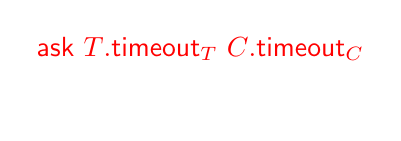
\begin{tikzpicture}[shorten >=1pt,node distance=.7cm,>=stealth']
      \node (start) {\color{red}\PortAsk\ \NameTimer.\PortTOT\ \NameCtrl.\PortTOC};
      \node()[below of=start]{};
    \end{tikzpicture}
%
    &
%
    $
    \begin{array}[b]{c@{}}
      {\color{red}
        \begin{aligned}
          \NameCtrl.\PortTOC &\Rightarrow
          \PortAsk \land \NameTimer.\PortTOT
          \\
          \NameTimer.\PortTOT &\Rightarrow 
          \PortAsk \land \NameCtrl.\PortTOC
        \end{aligned}}
      \\[11pt]
      {\color{red}
        \begin{aligned}
          \PortAsk &\Rightarrow
          \NameTimer.\PortTOT \land \NameCtrl.\PortTOC
          \\
          \true &\Rightarrow
          \PortAsk \land \NameTimer.\PortTOT
          \land \NameCtrl.\PortTOC
        \end{aligned}

      }
    \end{array}
    $
    %
    \\\hline
%
    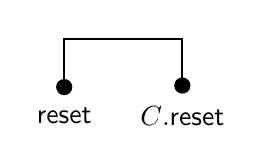
\begin{tikzpicture}[shorten >=1pt,node distance=.7cm,>=stealth']

      \node (start) {};
      \node(h4)[left of=start]{}; %, node distance=1.5cm

      \node[node distance=1cm] (ab) [below of=start] {\NameCtrl.\PortReset};
      \node[node distance=1.5cm] (aa) [left of=ab]{\PortReset};

      \draw [style=-*, thick, black]  ($(h4.south)+(0,.1cm)$) -| (ab.north);
      \draw [style=-*, thick, black]  ($(h4.south)+(0,.1cm)$) -| (aa.north);
    \end{tikzpicture}
%
    &
%
    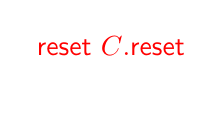
\begin{tikzpicture}[shorten >=1pt,node distance=.7cm,>=stealth']
      \node (start) {\color{red}\PortReset\ \NameCtrl.\PortReset};
      \node()[below of=start]{};
    \end{tikzpicture}
%
    &
%
    {\color{red}$
    \begin{aligned}[b]
      \NameCtrl.\PortReset &\Rightarrow \PortReset
      \\
      \PortReset &\Rightarrow \NameCtrl.\PortReset
      \\
      \true &\Rightarrow
      \PortReset \land \NameCtrl.\PortReset
    \end{aligned}
    $}
%
    \\\hline
  \end{tabular}}
\end{table}

Below, we assume that, as in \fig{schema:ArchFailure:BIP}, the
interaction model is defined by a set of connectors, annotated with
Boolean guards and with update assignments.  In particular, we assume
that the guards and update assignments are well-defined for any
interaction allowed by the connector.  For example, the choice
$\NameCtrl.\PortFail\ ?\ \NameCtrl.\mathit{zone} : \topinterval$ in
the update assignement
\[
\NameTimer.\mathit{z} := \NameTimer.\mathit{z}
\cap \Big(
\bigl(
\NameCtrl.\PortFail\ ?\ \NameCtrl.\mathit{zone} : \topinterval
\bigr)
+ \NameTimer.\mathit{t} \Big)
\]
associated to the connector {\NameTimer.\PortTick \trigsynch
  (\PortFail \trigsynch \NameCtrl.\PortFail)} in
\fig{schema:ArchFailure:BIP} ensures that the assignment is
well-defined independently of whether {\NameCtrl.\PortFail}
participates or not.  Let us denote by $\gamma \subset \ac(P_A)
\times \guards{V_A} \times \assigns{V_A}$ the set of connectors in the
architecture $A$ and by $P_x$ the set of ports involved in the
connector $x \in \gamma$.  Then, we have
\begin{align*}
  \gamma &=
  \setdef{(x, g, u)}{x \in \ac(P_x), g \in \guards{V_x}, u \in
    \assigns{V_x}}
  \\
  &\simeq \setdef{(a,g,u)}{(x,g,u) \in \gamma, a \in \intsem{x}}
  = \Gamma
  \,.
\end{align*}

We first define the encoding of $\Gamma$ as $\nopri[\Gamma] \bydef{=}
\setdef{\nopri[x,g,u]}{(x,g,u) \in \gamma}$, where $\nopri[x,g,u]$ is the synchronisation vector defined by
%
\begin{equation}
  \label{eq:nopri:connector}
  \nopri[x,g,u] \bydef{=}
  \bigl(p(b_p,\export[A](p))\bigr)^{p \in P_x}
  \rightarrow
  \alpha_p
  \left[\bigwedge R(\tau(x))\bigl[\nicefrac{b_p}{p}\bigr]\right]
  \,,
\end{equation}
%
with $b_p$ a fresh Boolean variable, $\alpha_p$ a fresh name, $\tau :
\ac(P_A) \rightarrow \ct(P_A)$ and $R : \ct(P_A) \rightarrow
\cru(P_A)$ the two mappings defined in \app{transformations} and
illustrated in \tab{connectors}, $\bigl[\nicefrac{b_p}{p}\bigr]$ is
the substitution, which replaces, in the expression that preceeds it,
all occurrences of $p$ by $b_p$.

\todoLHin{The update assignment is missing from the above encoding.
  It should be $u\bigl[\nicefrac{b_p}{p}\bigr]$, but I do not see in
  \defn{pnets} where should I place it.  I think it is missing there.
  \Simon}

\begin{theorem}
  The open automaton $\semopen{\nopri[A,\partition]}$ corresponding to
  $\nopri[A,\partition]$ (see \defn{operationalSemantics}) is
  isomorphic to the LTS $\semopen{\Gamma\bigl(\cC_A, (B_D)^{D \in
      \partition}\bigr)}$ (see \defn{comp:semantics}), where, for each
  $D \in \partition$, the component $B_D \bydef{=} \tuple{\{q\}, q,
    V_D, \val{0}{D}, D, \export[D], \goesto{}}$, with
%
  \begin{align*}
    V_D &= \bigcup_{p \in D} \export[A](p)
    \,,
    &\val{0}{D}(v) &= \bot, \text{ for all $v \in V_D$}
    \,,\\
    \goesto{} &= \bsetdef{(q, p, \true, \noop, q)}{p \in D}
    \,,
    &\export[D](p) &= \export[A](p), \text{ for all $p \in D$}
    \,,
  \end{align*}
%
  and $q$ a fresh state.
\end{theorem}
%
\begin{proof}[Sketch of a proof]
  The theorem follows from the correctness of $\tau$ and $R$ shown in
  \cite{BliSif10-causal-fmsd}.
\end{proof}

\noteSBin{This theorem is very probably correct: the key question is
  whether isomorphism is, indeed, the relation to use. In absence of
  silent transitions, must be the case.}


Observe now that this encoding can be optimised to remove unnecessary
Boolean variables and loop transitions marked by \false.  For
instance, consider the ports shown in red in the second column of
\tab{connectors}.  All these ports only appear in the roots of the
corresponding causal interaction trees and, furthermore, each of these
trees only has one root (see \app{trees}).  In such cases, as in the
{\NameTimer.\PortTick \trigsynch (\PortFail \trigsynch
  \NameCtrl.\PortFail)} example discussed above, the Boolean variables
and the \false-marked loop transitions associated to these ports can
be removed.  Furthermore, the rules associated to these ports in the
corresponding systems of causal rules (see the rules in red in the
third column of \tab{connectors}) become tautological and can also be
removed from the corresponding guards in \eq{nopri:connector}.

%****************************************************************
\subsection{Encoding with the maximal progress priority model}
\label{secn:enc:maxprog}

\noteSBin{In order to encode the maximal progress priority model, one
  has to introduce an additional Boolean variable, for each port (for
  which we have introduced one in $\nopri[A, \partition]$), such that
  $q \goesto{p(b_p, \true)} q'$ iff $\exists q'': q \goesto{p(\true)}
  q''$ in $\nopri[A, \partition]$.  Intuitively, this variable
  indicates whether \emph{there is a possibility to fire $p$ from the
    same state}.  Then, in the SV guard, we have to check whether
  \emph{all ports in $c_p(\tau(x))$ can be fired} (see
  \app{transformations}).  If so, then $p$ must be fired, \ie
  $p(\false)$ must be blocked.  This is pretty much straightforward,
  but care must be taken when doing this in the general case, since
  causal interaction trees can get pretty tricky due to $\oplus$ (see
  \app{trees}).}
%****************************************************************
%****************************************************************

\subsection{SMT encoding of open pNets}
\label{secn:smt}

%****************************************************************
%****************************************************************

\section{Case study}
\label{secn:case-study}

%****************************************************************

\subsection{Verification of the characteristic properties}
\label{secn:arch:verif}

\begin{figure}[t]
  \centering
  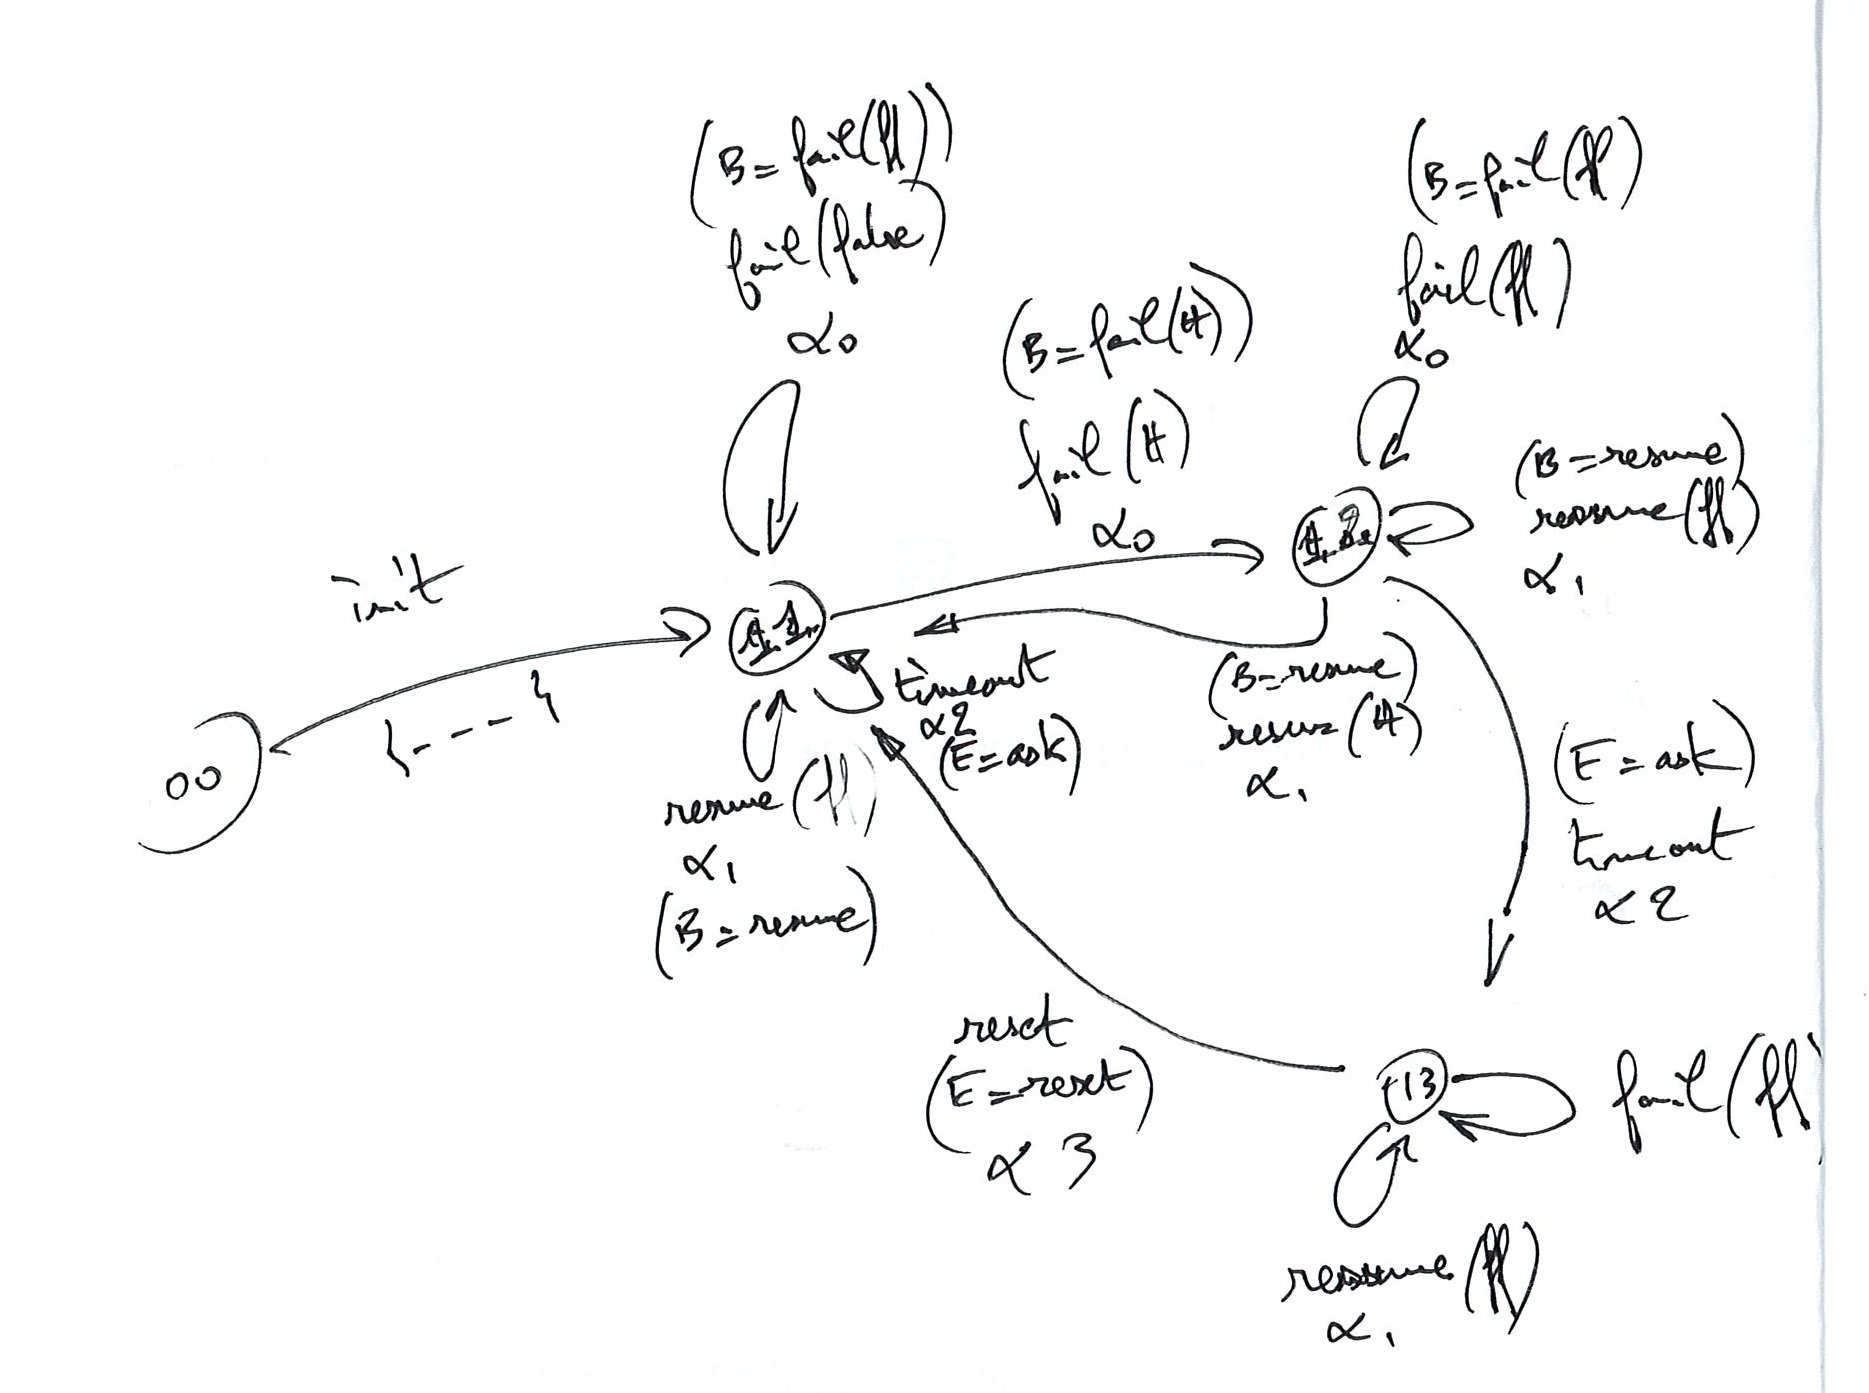
\includegraphics[width=\columnwidth]{TimerOpenAut}
  \caption{The open Automaton of the Failure Monitor Architecture}
  \label{schema:ArchFailure:BIP}
\end{figure}

\begin{figure}[t]
  \centering
  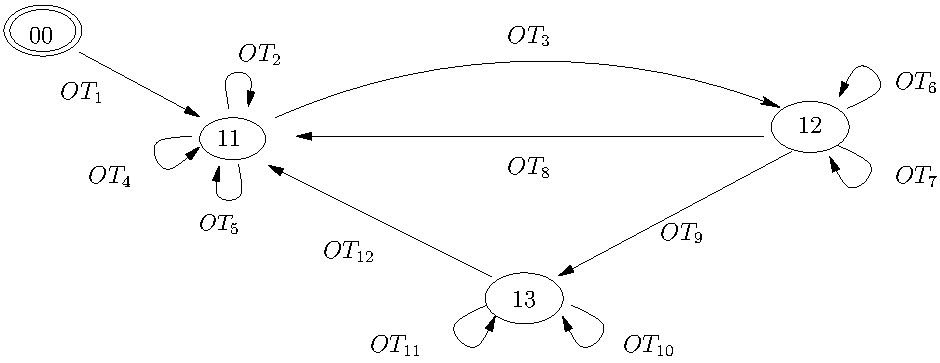
\includegraphics[width=0.8\columnwidth]{FailureTimerOA}
  \caption{The open Automaton of the Failure Monitor Architecture}
  \label{schema:ArchFailure:BIP}
\end{figure}

12 open transitions... Comments on the predicates ???

Should list some temporal logic properties....

%****************************************************************

\subsection{Composition of architectures}
\label{secn:arch:composition}

We now consider a system comprising two components $B_1$ and $B_2$
with the corresponding interfaces $\tuple{V_i, P_i,
  \export[i]}_{i=1,2}$, such that $\listset{\PortFail_i,
  \PortResume_i} \subseteq P_i$, for $i = 1,2$.

Assuming that the associated system requirements comprise the
capability of monitoring the failure events corresponding to ports
$\PortFail_1$ and $\PortFail_2$ of the two components, we would like
to apply two instances of the Failure Monitor architecture.  However,
we impose an additional constraint: only one timer coordinator is
allowed, for example because it must eventually be implemented by a
hardware component.

We consider two architecture instances $A_i = \tuple{\cC_i, V_{A_i},
  P_{A_i}, \export[A_i], \Gamma_i}$, for $i = 1,2$, with all their
constituting elements cloned from the Failure Monitor architecture of
the previous examples while substituting each entity $X$ by $X^i$.
For instance, the initialisation of the $\mathit{zone}$ variable is
transformed into $\IntervalInit[1]$ and $\IntervalInit[2]$,
respectively.  The only exception to this cloning procedure are the
sets of coordinating components: $\cC^i = \listset{\NameTimer,
  \NameCtrl^i}$, \ie the $\NameTimer$ component is shared, while
components $\NameCtrl^1$ and $\NameCtrl^2$ are obtained by making two
copies of $\NameCtrl$ as above.

In order to apply both architectures, we must verify that they are
upwards compatible and compute the combined interaction model $\Gamma$
in $A_1 \arcomp A_2 = \tuple{\cC_1 \cup \cC_2, V_{A_1} \cup V_{A_2},
  P_{A_1} \cup P_{A_2}, \export[A_1] \cup \export[A_2], \Gamma}$
(see \defn{arch:composition}).

%****************************************************************
%****************************************************************

\section{Related work}
\label{secn:related}
Previous works on pNets and BIP architectures have been mentioned at the beginning of the paper. Consequently, we  review here the closest related works outside the scope of pNets and BIP architectures. Among those, we focus on existing approaches for the compositional and parameterized verification of systems, and on alternative verification engines???
\noteLH{not sure about this classification ; to be refined}

A few tracks

%%% compositional verification
approaches by typing interfaces/protocols

infinite/parametrized model checking?

theorem proving? (too much manual effort) we need an example, we could cite Coqcots and Pycots for reconfiguration

SMT on an application not using component structure. is there a strong Z3 example

KeY? (I would call this symbolic execution and assume-guarantee)







%****************************************************************

%****************************************************************

\section{Conclusion}
\label{secn:conclusion}

%****************************************************************
%****************************************************************

\bibliographystyle{abbrv}
\bibliography{biblio}

%****************************************************************
%****************************************************************
\appendix
\clearpage

%****************************************************************
%****************************************************************

\section{Proofs}
\label{secn:proofs}

\begin{lemma}
  \label{lem:onlyone}
  Let $A = \tuple{\cC, V_A, P_A, \export[A], \Gamma}$ be an architecture and denote
  by $\Gamma_\cC \bydef{=}
%
  \setdef{
    (a \cap P_\cC, \true, \noop)
  }{
    (a, g, e) \in \Gamma
  }$, with $P_\cC = \bigcup_{C \in \cC} P_C$,
%  
  the projection of $\Gamma$ onto the coordinating components of
  $A$.  Consider the architecture $A' = \tuple{\{C'\}, V_A, P_A, \export[A],
  \Gamma}$, where $C' = \Gamma_\cC(\cC)$.  For any set of
  components $\cB$, satisfying the conditions of
  \defn{arch:application}, we have
  $\semopen{A(\cB)} = \semopen{A'(\cB)}$.
\end{lemma}
%
\begin{proof}
  First of all, notice that, by \defn{im:sem},
  $V_{C'} = \bigcup_{C \in \cC} V_C$ and $P_{C'} = P_\cC = \bigcup_{C \in \cC} P_C$.
  The conditions of \defn{arch} are satisfied and $A'$ is indeed
  an architecture.  Furthermore, $\cB$ satisfies the conditions
  of \defn{arch:application} \wrt $A'$.  Hence, the component
  $A'(\cB)$ is well defined.

  Clearly the state spaces and initial states %% and interfaces
  of both LTSs $\semopen{A(\cB)}$ and $\semopen{A'(\cB)}$
  coincide.  Thus, we only have to prove that so do the
  transition relations.  Let us assume that
  $\cC = C_i^{i \in I}$ and $\cB = B_j^{j \in J}$.
  We will use $q_i, q_i'$ to denote the states of
  $C_i$ and $q_j, q_j'$ to denote the states of $B_j$,
  and similarly for the valuations of variables.

  By \defn{comp:semantics},
%
  \begin{equation}
    \label{eq:lem1:trans:sem}
    (q_i, \val{}{i})^{i \in I} (q_j, \val{}{j})^{j \in J}
    \goesto{a, \val[\tilde]{}{}}
    (q_i', \val{\prime}{i})^{i \in I}
    (q_j', \val{\prime}{j})^{j \in J}
  \end{equation}
%  
  is a transition in $\semopen{A(\cB)}$ (\resp
  $\semopen{A'(\cB)}$) iff
%
  \begin{equation}
    \label{eq:lem1:trans}
    q_i^{i \in I} q_j^{j \in J}
    \goesto{a, g', e'}
    (q_i')^{i \in I} (q_j')^{j \in J}
    \,,
  \end{equation}
%
  is a transition in $A(\cB)$ (\resp $A'(\cB)$) and
%
  \begin{mathpar}
    \val{i \in I}{i} \val{j \in J}{j}
    \models g'
    \,,
    \and
    (\val{\prime}{i})^{i \in I} (\val{\prime}{j})^{j \in J}
    = \val[\tilde]{}{}[e']
    \,,
    \and
    \valdiff{\val{i \in I}{i} \val{j \in J}{j}}{
      \val[\tilde]{}{}} \subseteq \export(a)       
  \end{mathpar}
%
  (with $\export$ defined as in \defn{arch:application}).

  By \defn{im:sem} and \defn{priority:sem}, \eq{lem1:trans} is a transition in $A(\cB)$
  iff $a \neq \emptyset$, $(a, g, e) \in \IMextend{\Gamma}{P}$,
  where $P = \bigcup_{B \in \cB \cup \cC} P_B$, and
  %
  \begin{enumerate}
  \item\label{ab:start} for $i \in I$,\\
    $a \cap P_{C_i} \neq \emptyset$ and
    $q_i \goesto{a \cap P_{C_i},\, g_{C_i},\, e_{C_i}} q_i'$
    is a transition in $C_i$, or\\
    $a \cap P_{C_i} = \emptyset$ and $q_i = q_i'$
    (for covenience, we put $g_{C_i} = \true$ and $e_{C_i} = \noop$ in item~\ref{aux1} below);
  \item for $j \in J$,\\
    $a \cap P_{B_j} \neq \emptyset$ and
    $q_j \goesto{a \cap P_{B_j},\, g_{B_j},\, e_{B_j}} q_j'$
    is a transition in $B_j$, or\\
    $a \cap P_{B_j} = \emptyset$ and $q_j = q_j'$
    (for covenience, we put $g_{B_j} = \true$ and $e_{B_j} = \noop$ in item~\ref{aux1} below);
  \item\label{ab:end}\label{aux1} $g' = g \land \bigwedge_{i \in I} g_{C_i} \land
    \bigwedge_{j \in J} g_{B_j} \land \varphi_\mu$ and
    $e' = e; e_{C_i}^{i \in I}, e_{B_j}^{j \in J}$, where    
%
    \begin{equation}
      \label{eq:only1:maxprog:guard}
      \varphi_\mu = \bigwedge_{
        \begin{array}{c}
          q_i^{i \in I} q_j^{j \in J} \goesto{b, h, f} \text{ in }
          (\IMextend{\Gamma}{P})(\cC \cup \cB)
          \\
          a \varsubsetneq b
        \end{array}
      } \lnot h
      \,.
    \end{equation}
%
  \breakenumistart

  Similarly, \eq{lem1:trans} is a transition in
  $A'(\cB)$ iff $a \neq \emptyset$,
  $(a, g, e) \in \IMextend{\Gamma}{P}$ and
%
  \breakenumiend
% 
  \item \label{a1b:start} \label{only1:coord}
    $a \cap P_{C'} \neq \emptyset$ and 
    $(q_i)^{i \in I} \goesto{a \cap P_{C'}, g_{C'}, e_{C'}} (q_i')^{i \in I}$
    is a transition in $C'$, or\\
    $a \cap P_{C'} = \emptyset$ and $q_i = q_i'$,
    for all $i \in [1,m]$
    (for covenience, we put $g_{C'} = \true$ and $e_{C'} = \noop$ in
    item~\ref{aux2} below);
  \item for $j \in J$,\\
    $a \cap P_{B_j} \neq \emptyset$ and
    $q_j \goesto{a \cap P_{B_j}, g_{B_j}, e_{B_j}} q_j'$
    is a transition in $B_j$, or\\
    $a \cap P_{B_j} = \emptyset$ and $q_j = q_j'$
    (for covenience, we put $g_{B_j} = \true$ and $e_{B_j} = \noop$ in
    item~\ref{aux2} below);
  \item\label{aux2} $g' = g \land g_{C'} \land
    \bigwedge_{j \in J} g_{B_j} \land \varphi_\mu'$ and
    $e' = e; e_{C'}, e_{B_j}^{j \in J}$ (with $\varphi_\mu'$ defined as
    in \eq{only1:maxprog:guard}, but substituting $\{C'\}$ instead of $\cC$).
%
  \breakenumistart
  Notice that, for any $i \in I$, since
  $P_{C_i} \subseteq P_{C'}$, we have
  $a \cap P_{C_i} = (a \cap P_{C'}) \cap P_{C_i}$.
  Thus, if $a \cap P_{C'} \neq \emptyset$, 
  the transition in condition~\ref{only1:coord} above is
  present in $C'$ iff
  $(a \cap P_{C'}, \true, \noop) \in \Gamma_\cC$ and
  \breakenumiend
% 
  \item for $i \in I$,\\
    $a \cap P_{C_i} \neq \emptyset$ and
    $q_i \goesto{a \cap P_{C_i}, g_{C_i}, e_{C_i}} q_i'$
    is a transition in $C_i$, or\\
    $a \cap P_{C_i} = \emptyset$ and $q_i = q_i'$,
    (for covenience, we put $g_{C_i} = \true$ and $e_{C_i} = \noop$ in
    item~\ref{aux3} below);
  \item \label{a1b:end} \label{aux3} $g_{C'} = \bigwedge_{i \in I} g_{C_i}$ and
    $e_{C'} = e_{C_i}^{i \in I}$.
  \end{enumerate}

  Consider $(a,g,e) \in \IMextend{\Gamma}{P}$.  By
  \eq{im:extension}, this is equivalent to
  $(a \cap P_A, g, e) \in \Gamma$.
  Since $P_{C'} = P_\cC \subseteq P_A$, we have
  $a \cap P_{C'} = a \cap P_\cC = (a \cap P_A) \cap P_\cC$.
  Hence, by the definition of $\Gamma_\cC$ in the lemma statement,
  this is also equivalent to
  $(a \cap P_{C'}, \true, \noop) \in \Gamma_\cC$.

  Thus, conditions \ref{ab:start}\ndash\ref{ab:end} are satisfied iff
  so are conditions \ref{a1b:start}\ndash\ref{a1b:end} (to see that
  $\varphi_\mu$ is satisfied iff so is $\varphi_\mu'$, one has to
  consider the same two sets of conditions, but this time without the
  additional conjuncts $\varphi_\mu$ and $\varphi_\mu'$ in
  items~\ref{aux1} and \ref{aux2}, since no priority model is applied
  to obtain $C'$).  This proves that the transition relations of
  $\semopen{A(\cB)}$ and $\semopen{A'(\cB)}$ coincide and, therefore,
  $\semopen{A(\cB)} = \semopen{A'(\cB)}$.
\end{proof}

\begin{note}
  \label{rem:upwards:compat}
  Notice that, since, in the statement of \lem{onlyone}, 
  %
  \begin{enumerate}
  \item the interaction models are the same for both $A$ and $A'$, and
  \item $P_{C'} = P_\cC$,
  \end{enumerate}
  %
  substituting $A'$ for $A$ preserves upwards compatibility, \ie for any
  architecture $A''$, holds the following statement: $A$ and $A''$ are
  upwards compatible if and only if so are $A'$ and $A''$.
\end{note}

\begin{lemma}
  \label{lem:onestep}
  Let $\cB$ be a set of components; let $A_i = \tuple{\{C_i\}, V_{A_i},
  P_{A_i}, \export[A_i], \Gamma_i}$, for $i = 1,2$, be two upwards compatible architectures
  with one coordinator each, applicable to $\cB$.  Denote
  $P_i = P_{C_i} \cup \bigcup_{B \in \cB} P_B$.
  Finally, let
%
  $
  s_1 s_2 s
%
  \goesto{a, \tilde{\val{}{}}}
%
  s_1' s_2' s'
  $,
%
  be a transition in $\semopen{(A_1 \arcomp A_2)(\cB)}$, with
  $a \neq \emptyset$, 
  $s, s' \in \prod_{B \in \cB} S_{\semopen{B}}$
  and
  $s_i, s_i' \in S_{\semopen{C_i}}$ ($i=1,2$).
%
  Then, for $i=1,2$, either $a \cap P_i = \emptyset$ and $s_i s=
  s_i' s'$, or there exists a transition
%
  $
  s_i s
%
  \goesto{a \cap P_i, \val[\doubletilde]{}{}}
%
  s_i' s''
  $ 
%
  in $\semopen{A_i(\cB)}$, with
  $\val[\doubletilde]{}{}$ being the restriction of
  $\val[\tilde]{}{}$ to
  $V_i = V_{C_i} \cup \bigcup_{B \in \cB} V_B$ and
  $s' \order s''$.
\end{lemma}
%
\begin{proof}
  By \defn{comp:semantics}, every semantic state consists of a
  component state and a valuation of component variables.  Thus,
  we can expand $s_1 s_2 s \goesto{a, \tilde{\val{}{}}} s_1' s_2' s'$
  as
%
  \[
  (q_1, \val{}{1}, q_2, \val{}{2}, q, \val{}{})
%
  \goesto{a, \tilde{\val{}{}}}
%
  (q_1', \val[\primeit]{}{1}, q_2', \val[\primeit]{}{1}, q', \val[\primeit]{}{})
  \,.
  \]
%
  By \defn{im:sem} and \defn{priority:sem}, this implies
  that
  $(q_1, q_2, q) \goesto {a, g', e'} (q_1', q_2', q')$
  is a transition in $(A_1 \arcomp A_2)(\cB)$, with
%
  $g' = g \land g_1 \land g_2 \land g_\cB \land \varphi_\mu$
  and
  $e' = e; (e_1, e_2, e_\cB)$,
  where $(a, g, e) \in \Gamma$ (see \eq{arch:composition} for the
  definition of $\Gamma$);
%  
  $g_1$, $g_2$ and $e_1$, $e_2$ are, respectively, the guards and
  update expressions of the underlying transitions in the coordinating
  components $C_1$ and $C_2$;
%    
  \begin{mathpar}
    g_\cB = \bigwedge_{B \in \supp{a} \cap \cB} g_B
    \,,
    \and
    e_\cB = e_B^{B \in \supp{a} \cap \cB}
    \,,
  \end{mathpar}
%
  are the compositions of, respectively, the guards and update
  expressions of the operand components;
%    
  \begin{equation}
    \label{eq:onestep:maxprog:guard}
    \varphi_\mu = \bigwedge_{
      \begin{array}{c}
        (q_1, q_2, q) \goesto{b, h', f'} \text{ in }
        \bigl(\IMextend{\Gamma}{(P_1 \cup P_2)}\bigr)
        \bigl(\{C_1, C_2\} \cup \cB\bigr)
        \\
        a \varsubsetneq b
      \end{array}
    } \lnot h'
  \end{equation}
%
  is the conjunct encoding the maximal progress priority in
  \defn{priority:sem}.  As above for $g'$, for each $(b, h', f')$ in
  \eq{onestep:maxprog:guard}, $h'$ can be decomposed as $h' = h \land
  h_1 \land h_2 \land h_\cB$ (without the maximal progress conjunct,
  since no priority is applied in $\bigl(\IMextend{\Gamma}{(P_1 \cup
    P_2)}\bigr)\bigl(\{C_1, C_2\} \cup \cB\bigr)$).
  
  By \eq{comp:semantics}, we also have
%
  \begin{align}
    \label{eq:guard}
    (\val{}{1}, \val{}{2}, \val{}{}) &\models g'
    \,,
    \\
    \label{eq:substitution}
    (\val[\primeit]{}{1}, \val[\primeit]{}{2}, \val[\primeit]{}{})
    &= \val[\tilde]{}{}[e']
    \,,
    \\
    \label{eq:transient}
    \valdiff{(\val{}{1}, \val{}{2}, \val{}{})}{\val[\tilde]{}{}}
    &\subseteq \export(a)
    \,.
  \end{align}
%
  If $a \cap P_1 = \emptyset$, then $\supp{a} = \{C_2\}$ and, by
  \eq{transient} and \defn{im:sem}, $s_1 = s_1'$ and $s = s'$
  (recall, \defn{im}, that, for $(a,g,e) \in \Gamma$, we have $e
  \in \exprs{V_a}$).  Hereafter, assume $a \cap P_1 \neq
  \emptyset$.

  By \eq{arch:composition}, for $i=1,2$, there exist $(a \cap P_{A_i},
  g^i, e^i) \in \Gamma_i$, such that $g = g^1 \land g^2$ and $e = e^1
  \land e^2$.
  %% Similarly, for each $(b, h', f')$ in \eq{onestep:maxprog:guard},
  %% there exist $(b \cap P_{A_i}, h^i, f^i) \in \Gamma_i$, such that
  %% $h = h^1 \land h^2$ and $f = f^1 \land f^2$.
%
  We want to show that the interaction $(a \cap P_1, g^1, e^1)$ is
  enabled in the state $(q_1, \val{}{1}, q, \val{}{})$ of
  $\semopen{A_1(\cB)}$.  To this end, we proceed in two steps:
%
  \begin{enumerate}
  \item \label{onestep:proof:im} We show that $(a \cap P_1, g^1,
    e^1)$ is enabled in the state $(q_1, \val{}{i}, q, \val{}{})$ of
    $\semopen{(\IMextend{\Gamma_1}{P_1})(\cB)}$.
  \item \label{onestep:proof:maxp} We show that $(a \cap P_1, g^1,
    e^1)$ is not inhibited in $\semopen{A_1(\cB)} =
    \semopen{\mu\bigl((\IMextend{\Gamma_1}{P_1})(\cB)\bigr)}$ by the
    maximal progress priority.
  \end{enumerate}

  \paragraph*{Step \ref{onestep:proof:im}}
  %% Denoting $P_\cB = \bigcup_{B \in \supp{a} \cap \cB} P_B$, 
  By \defn{im:sem}, we have
%
  \begin{mathpar}
    q_1 \goesto{a \cap P_{C_1}, g_1, e_1} q_1'
    \and
    \text{and}
    \and
    q_B \goesto{a \cap P_B, g_B, e_B} q_B',
    \text{ for each }
    B \in \cB
    \,.
  \end{mathpar}

  By \eq{guard}, we have
  $(\val{}{1}, \val{}{}) \models g^1 \land g_1 \land g_\cB$.

  Denoting \todoSB{One tilde is enough}$\val[\doubletilde]{}{1}$ the restriction of
%
  $\val[\tilde]{}{}$ to
  $V_1 = V_{C_1} \cup \bigcup_{B \in \cB} V_B$,
%
  we have, by \eq{substitution} and the monotonicity of
  expressions,
%
  $(\val[\primeit]{}{1}, \val[\primeit]{}{}) \order
  \val[\doubletilde]{}{1}[e^1; (e_1, e_b)]$.  \todoSB{Remove this}\hl{Notice that all
  variables affected by both $e^1$ and $e^2$ must necessarily
  belong to $\bigcup_{B \in \cB} V_B$.}  Hence,
%
  $\val[\doubletilde]{}{1}[e^1; (e_1, e_b)] =
  (\val[\primeit]{}{1}, \val[\secondit]{}{})$ with 
  $\val[\primeit]{}{} \order \val[\secondit]{}{}$.

  By \defn{comp:semantics} and \defn{im:sem}, we have
  $
  (q_1, \val{}{1}, q, \val{}{})
  \goesto{a \cap P_1, \val[\doubletilde]{}{1}}
  (q_1', \val[\primeit]{}{1}, q, \val[\secondit]{}{})
  $ in $\semopen{(\IMextend{\Gamma_1}{P_1})(\cB)}$.

  Symmetrically, we have 
  $
  (q_2, \val{}{2}, q, \val{}{})
  \goesto{a \cap P_2, \val[\doubletilde]{}{2}}
  (q_2', \val[\primeit]{}{2}, q, \val[\secondit]{}{})
  $ in $\semopen{(\IMextend{\Gamma_2}{P_2})(\cB)}$.   
   
  \paragraph*{Step \ref{onestep:proof:maxp}}
  Suppose that $a \cap P_1 \varsubsetneq b_1$, for some interaction
  $(b_1, h^1, f^1) \in \IMextend{\Gamma_1}{P_1}$ enabled in $(q_1,
  \val{}{1}, q, \val{}{})$.  Then, by upwards compatibility of $A_1$
  and $A_2$, there exists $(b_2, h^2, f^2) \in
  \IMextend{\Gamma_2}{P_2}$, enabled in $(q_2, \val{}{2}, q,
  \val{}{})$, such that $a \cap P_2 \subseteq b_2$ and $b_2 \cap P_1 =
  b_1 \cap P_2$.  By \eq{im:extension}, we have $(b_1 \cap P_{A_1},
  h^1, e^1) \in \Gamma^1$.  Furthermore,
%
  \begin{multline*}
    ((b_1 \cap P_{A_1}) \cup (b_2 \cap P_{A_2}))  \cap P_{A_1} =
    (b_1 \cap P_{A_1}) \cup (b_2 \cap P_{A_1} \cap P_{A_2}) =\\
    (b_1 \cap P_{A_1}) \cup ((b_2 \cap P_1) \cap P_{A_1} \cap P_{A_2}) =  
    (b_1 \cap P_{A_1}) \cup ((b_1 \cap P_2) \cap P_{A_1} \cap P_{A_2}) =\\
    (b_1 \cup (b_1 \cap P_2 \cap P_{A_2})) \cap P_{A_1} =
    b_1 \cap P_{A_1} 
  \end{multline*}
%
  Symmetrically, $(b_2 \cap P_{A_2}, h^2, e^2) \in \Gamma^2$ and
  $((b_1 \cap P_{A_1}) \cup (b_2 \cap P_{A_2})) \cap P_{A_2} = b_2
  \cap P_{A_2}$.  By \eq{arch:composition}, we then have $((b_1 \cap
  P_{A_1}) \cup (b_2 \cap P_{A_2}), h^1 \land h^2, f^1 \expmix f^2)
  \in \Gamma$ and, by \eq{im:extension}, $(b_1 \cup b_2, h^1 \land
  h^2, f^1 \expmix f^2) \in \IMextend{\Gamma}{(P_1 \cup P_2)}$.
%
  Since both $(b_i, h^i, f^i) \in \IMextend{\Gamma_i}{P_i}$ are
  enabled in the respective states $(q_i, \val{}{i}, q, \val{}{})$, we
  conclude that $(b_1 \cup b_2, h^1 \land h^2, f^1 \expmix f^2)$ is
  enabled in $(q_1, \val{}{1}, q_2, \val{}{2}, q, \val{}{})$.

  Since $a \cap P_1 \varsubsetneq b_1$ and $a \cap P_2 \subseteq b_2$,
  we have $a \varsubsetneq b_1 \cup b_2$.  Thus, $(b_1 \cup b_2, h^1
  \land h^2, f^1 \expmix f^2)$ contribute to $\varphi_\mu$ in
  \eq{onestep:maxprog:guard}.  Since $(b_1 \cup b_2, h^1 \land h^2,
  f^1 \expmix f^2)$ is enabled in $(q_1, \val{}{1}, q_2, \val{}{2}, q,
  \val{}{})$, we have $(\val{}{1}, \val{}{2}, \val{}{}) \models h^1
  \land h^2$ and, therefore $(\val{}{1}, \val{}{2}, \val{}{})
  \not\models \varphi_\mu$, which contradicts \eq{guard}, thereby
  proving that $(a \cap P_1, g^1, e^1)$ is not inhibited in
  $\semopen{A_1(\cB)} =
  \semopen{\mu\bigl((\IMextend{\Gamma_1}{P_1})(\cB)\bigr)}$ by the
  maximal progress priority.

  The corresponding statement for $(a \cap P_2, g^2, e^2)$ is obtained
  symmetrically.
\end{proof}

\begin{lemma}
  \label{lem:stepabove}
  Consider a component $B$ and let 
%
  $
  (q_1, \val{}{1})
%
  \goesto{a, \val[\tilde]{}{}}
%
  (q_2, \val{}{2})
  $,
%
  be a transition in $\semopen{B}$.  For any valuation
  $\val[\primeit]{}{1}$, such that
  $\val{}{1} \order \val[\primeit]{}{1}$ and
  $\valdiff{\val{}{1}}{\val[\primeit]{}{1}} \subseteq \export(a)$,
  there exists a transition
%
  $
  (q_1, \val[\primeit]{}{1})
%
  \goesto{a, \val[\tilde]{}{}}
%
  (q_2, \val{}{2})
  $
%
  in $\semopen{B}$.
\end{lemma}
%
\begin{proof}
  By \eq{comp:semantics}, we have
%
  \begin{mathpar}
    q_1 \goesto{a, g, e} q_2
    \,,
    \and
    \val{}{1} \models g
    \,,
    \and
    \val{}{2} = \val[\tilde]{}{}[e]
    \,,
    \and
    \text{and}
    \and
    \valdiff{\val{}{1}}{\val[\tilde]{}{}} \subseteq \export(a)
    \,.
  \end{mathpar}

  By monotonicity of guards, we deduce
  $\val[\primeit]{}{1} \models g$.
  For any $v \not\in \export(a)$,
  $\val[\primeit]{}{1}(v) = \val{}{1}(v) = \val[\tilde]{}{}(v)$.
  Hence, 
  $\valdiff{\val[\primeit]{}{1}}{\val[\tilde]{}{}}
  \subseteq \export(a)$.
  By \eq{comp:semantics}, we conclude 
%
  $
  (q_1, \val[\primeit]{}{1})
%
  \goesto{a, \val[\tilde]{}{}}
%
  (q_2, \val{}{2})
  $.  
\end{proof}

\begin{proof}[Proof of \thm{combining}]
  By \lem{onlyone}, we can assume without loss of generality that each of the two
  architectures has only one coordinating component.  For $i =
  1,2$, we denote $\{C_i\} = \cC_i$, $P_i = P_{C_i}
  \cup\ \bigcup_{B \in \cB} P_B$ and $V_i = V_{C_i}
  \cup\ \bigcup_{B \in \cB} V_B$.
%
  By \rem{upwards:compat}, this does not affect their upwards
  compatibility, hence neither does this affect the applicability of
  \lem{onestep} below.
  
  The initiality of $\Phi_1 \land \Phi_2$, is trivial: both
  $\Phi_1$ and $\Phi_2$ are initial, hence $s^0 \models \Phi_1
  \land \Phi_2$.

  Consider a path
%
  \[
  s^0_1 s^0_2 s^0
%
  \goesto{a^1, \val[\tilde]{1}{}}
%
  s^1_1 s^1_2 s^1
%
  \goesto{a^2, \val[\tilde]{2}{}}
  \cdots
  \goesto{a^k, \val[\tilde]{k}{}}
%
  s^k_1 s^k_2 s^k
  \]
%
  in $\semopen{(A_1 \arcomp A_2)(\cB)}$, where
  $s^0,\dots,s^k \in \prod_{B \in \cB} S_{\semopen{B}}$ and
  $s^0_i,\dots, s^k_i \in S_{\semopen{C_i}}$, for $i=1,2$.
  We have to show that $s^k \models \Phi_1 \land \Phi_2$.

  Assuming that $a^1 \cap P_1 \neq \emptyset$, by \lem{onestep},
  there exists $s^{1\prime} \in \prod_{B \in \cB} S_{\semopen{B}}$,
  such that
%
  \[
  s^0_1 s^0
%
  \goesto{a^1 \cap P_1, \val[\doubletilde]{1}{}}
%
  s^1_1 s^{1\prime}
  \]
%
  is a transition in $\semopen{A_1(\cB)}$ with
  $\val[\doubletilde]{1}{}$ being the restriction of
  $\val[\tilde]{1}{}$ to $V_1$ and
  $s^1 \order s^{1\prime}$.
%
  By \lem{stepabove}, 
  \[
  s^1_1 s^1_2 s^{1\prime}
%
  \goesto{a^2, \val[\tilde]{2}{}}
%
  s^2_1 s^2_2 s^2
  \]
  is a transition in $\semopen{(A_1 \arcomp A_2)(\cB)}$ and,
  therefore, 
  \[
  s^1_1 s^1_2 s^{1\prime}
%
  \goesto{a^2, \val[\tilde]{2}{}}
%
  s^2_1 s^2_2 s^2
%
  \goesto{a^3, \val[\tilde]{3}{}}
  \cdots
  \goesto{a^k, \val[\tilde]{k}{}}
%
  s^k_1 s^k_2 s^k
  \]
%  
  is a path in $\semopen{(A_1 \arcomp A_2)(\cB)}$.
%
  Notice that, if the above assumption, $a^1 \cap P_1 \neq
  \emptyset$, does not hold, then $s^0_1 = s^1_1$, $s^0 = s^1$
  and we can take $s^{1\prime} = s^1$ in this latter path.

  Repeating the entire argument $k-1$ times, starting with this
  shorter path, we obtain a path
%
  \begin{equation}
    \label{eq:path-in-1}
    s^0_1 s^0
    %
    \goesto{a^1 \cap P_1, \val[\doubletilde]{1}{}}
    %
    s^1_1 s^{1\prime}
    %
    \goesto{a^2 \cap P_1, \val[\doubletilde]{2}{}}
    %
    s^2_1 s^{2\prime}
    %
    \goesto{a^3 \cap P_1, \val[\doubletilde]{3}{}}
    \cdots
    \goesto{a^k \cap P_1, \val[\doubletilde]{k}{}}
    %
    s^k_1 s^{k\prime}
  \end{equation}
%  
  with $s^i \order s^{i\prime}$, for all $i \in [1,k]$.

  From \eq{path-in-1}, we conclude that the state $s^k_1
  s^{k\prime}$ is reachable in $\semopen{A_1(\cB)}$.  Since $A_1$
  enforces $\Phi_1$ on $\cB$, this implies that $s^{k\prime}
  \models \Phi_1$.  Since $s^k \order s^{k\prime}$, we deduce, by
  \defn{property}, that $s^k \models \Phi_1$.

  Symmetrically, $s^k \models \Phi_2$, which concludes
  the proof.
\end{proof}

%*********************************************************************
%*********************************************************************

\section{pNets additional definitions}
\label{secn:pNets:additional}

\begin{definition}[Sorts, Holes, Leaves of pNets]
  \begin{itemize}
  \item  \noteSB{I think this can be lightened up a bit, since the definitions are all 
  straightforward, whereas the notation is complex.  Maybe reformulate in words and move 
  the formal definitions in the appendix?}
 The sort of a pNet is its signature, i.e. the set of actions it can
perform. \noteSB{Is there any chance that, by writing assignments explicitly ($x := e$), 
we could eliminate the need to distinguish the input variables at all? That would 
simplify things.}\hl{In the definition of sorts, we do not need to distinguish
input variables} (that specify the dataflow within LTSs), so for
computing LTS sorts, we use a substitution operator\footnote{$\subst{y_k\gets x_k}^{k\in 
K}$ is the parallel substitution 
operation.} to remove the
\emph{input marker} of variables. Formally:
\[
\begin{array}{l}
\Sortop(\mylangle S,s_0, \to\myrangle) = \{\alpha\subst{x \gets ?x| 
x\in\symb{iv}(\alpha)}|s \xrightarrow{\langle \alpha,~g,~(x_j\!:= {e}_j)^{j\in
    J}\rangle} s'\in \to \} \\
\Sortop(\mylangle \overline{\pNet}\!, %\pNet_i^{i\in I}, \Sort_j^{j\in J}
\overline{\pNet}\!,
\overline{\symb{SV}}\myrangle)
=\{\alpha' |\, \overline{\alpha}%\alpha_j^{j\in J_k}
\to\alpha'\in\set{\symb{SV}}\}
\end{array}
\]

\item
The set of holes of a pNet is defined inductively; the sets of holes
in a pNet node and its subnets are all disjoint:
  \[\begin{array}{l}
\Holes(\mylangle S,s_0, \to\myrangle) \!=\! \emptyset \\
\Holes(\mylangle \pNet_i^{i\in I}\!,\Sort_j^{j\in J}\!, \overline{\symb{SV}}\myrangle) 
=J\uplus{\displaystyle \bigcup_{i\in 
I}\Holes(\pNet_i)}\\
\forall i\in I.\, \Holes(\pNet_i)\cap J=\emptyset\\
\forall i_1,i_2\in I.\,i_1\neq i_2\Rightarrow  
\Holes(\pNet_{i_1})\cap\Holes(\pNet_{i_2})=\emptyset
\end{array}\]
\item
The set of leaves of a pNet is the set of all pLTSs occurring in the structure, defined 
inductively as:
\[\begin{array}{l}
\Leaves(\mylangle S,s_0, \to\myrangle) \!=\!\emptyset\\%\{\mylangle S,s_0, \to\myrangle\}\\
\Leaves(\mylangle \pNet_i^{i\in I}\!,%Sort_j^{j\in J}
\overline{\Sort}\!, \overline{\symb{SV}}\myrangle) = {\displaystyle \biguplus_{i\in 
I}\Leaves(\pNet_i)\uplus\{i\mapsto \pNet_i|\pNet_i\pNet_i \text{ is a }\pLTS\}}
\end{array}\]
\end{itemize}
\end{definition}

%*********************************************************************
%*********************************************************************

\section{Algebraic representations of the interaction model}
\label{secn:algebras}

In this section condensed from
\cite[Section~4]{BarBliu15-offer-scico}, we briefly recall the syntax
and semantics of the algebras used to represent BIP interaction models
\emph{disregarding variables and data transfer}.  All the algebras are
parameterised by a set $P$ of all the ports in a given system.  The
semantics of the Algebra of Interactions $\ai(P)$ is given in terms of
sets of interactions by a function $\intsem{\cdot}: \ai(P) \rightarrow
2^{2^P}$.  The corresponding equivalence relation on $\ai(P)$ is
defined as follows: two terms $x,y \in \ai(P)$ are {\em equivalent} $x
\simeq y$ iff $\intsem{x} = \intsem{y}$.  For any other algebra
$\cA(P)$ among those appearing in this section, we define its
semantics by the function $\aisem{\cdot}: \cA(P) \rightarrow \ai(P)$.
A function $\intsem{\cdot}: \cA(P) \rightarrow 2^{2^P}$ is obtained by
composing $\aisem{\cdot}: \cA(P) \rightarrow \ai(P)$ and
$\intsem{\cdot}: \ai(P) \rightarrow 2^{2^P}$.  The axiomatisation of
$\ai(P)$ given in \cite{BliSif07-acp-emsoft} is sound and complete
with respect to $\simeq$.  Hence, for other algebras, the equivalences
induced by $\intsem{\cdot}$ and $\aisem{\cdot}$ coincide.

Below, we assume that a set of ports $P$ is given, such that $0,1\not\in
P$.

For any set $X$ of propositional variables, we denote by $\sB[X]$ the
corresponding Boolean algebra generated by $X$.  For presentation
clarity, we will often omit the conjunction operator and write $a \lor
bc$ instead of $a \lor (b \land c)$.


% *********************************************************************

\subsection{Algebra of Interactions}
\label{secn:ai}

The Algebra of Interactions is used to define the interaction semantics of other algebras. The elements of this algebra can be bijectively mapped to interaction models, \ie subsets of $2^P$.

\begin{syntax}
The syntax of the {\em Algebra of Interactions}, $\ai(P)$, is defined by
the following grammar
%
\begin{equation} \label{eq:apsynt}
  \begin{array}{rc*{4}{l@{\ |\ }}l}
    x & ::= & 0 & 1 & p \in P & x\cdot x & x + x \,,\\
  \end{array}
\end{equation}
%
where `$+$' and `$\cdot$' are binary operators, respectively called
{\em union} and {\em synchronisation}.  Synchronisation binds stronger
than union.
\end{syntax}
%
As follows from the interaction semantics given below, the additive
identity element $0$ represents blocking, since it does not authorise
any interaction.  The multiplicative identity element $1$ corresponds
to the empty interaction, which represents idling (see the discussion
in \cite{BarBliu15-offer-scico}).

\begin{semantics}
The semantics of $\ai(P)$ is given by the function $\|\cdot\| : \ai(P)
\rightarrow 2^{2^P}$, defined by
%
\begin{equation} \label{eq:apsem}
  \renewcommand{\arraystretch}{1.5}
  \begin{array}{lcl}
    \lefteqn{\|0\|\ =\ \emptyset,\quad \|1\|\ =\ \{\emptyset\},\quad
      \|p\|\ =\ \Big\{\{p\}\Big\},}\\
    \|x_1 + x_2\| &=& \|x_1\| \cup \|x_2\|,\\
    \|x_1 \cdot x_2\| &=& 
    \Big\{a_1 \cup a_2\,\Big|\, a_1\in \|x_1\|, a_2\in \|x_2\| \Big\},
  \end{array}
\end{equation}
for $p\in P$, $x_1,x_2\in\ai(P)$.  Terms of $\ai(P)$ represent sets of
interactions between the ports $P$.
\end{semantics}

A sound and complete axiomatisation of $\ai(P)$ with respect to the
semantic equivalence is provided in \cite{BliSif07-acp-emsoft}.  In a
nutshell, $(\ai(P), +, \cdot, 0, 1)$ is a commutative semiring,
idempotent in both $+$ and $\cdot$.


% *********************************************************************

\subsection{Algebra of Connectors}
\label{secn:ac}

The Algebra of Connectors provides an algebraic formalisation for
structuring the interaction models.  It underlies the graphical
notation (\eg \fig{connectors}) and the syntax for connectors used in the BIP language.

\begin{syntax}
The syntax of the {\em Algebra of Connectors}, $\ac(P)$, is defined by the
following grammar
%
\begin{equation} \label{eq:acsynt}
  \renewcommand{\arraystretch}{1.5}
  \begin{array}{lcll}
    s & ::= & [0]\ |\ [1]\ |\ [p]\ |\ [x] \:\:\:\:\:\:\:\:\:(synchrons)\\
    t & ::= & [0]'\ |\ [1]'\ |\ [p]'\ |\ [x]'  \:\:\:\:\:\:   (triggers)\\
    x & ::= & s\ |\ t\ |\ x\cdot x\ |\ x + x\,, 
  \end{array}
\end{equation}
for $p\in P$, and where `$+$' is a binary operator called {\em union},
`$\cdot$' is a binary operator called {\em fusion}, and brackets
`$[\cdot]$' and `$[\cdot]'$' are unary {\em typing} operators.  Fusion
binds stronger than union.

Union has the same meaning as union in $\ai(P)$. Fusion is a
generalisation of the synchronisation in $\ai(P)$.  Typing is used to
form typed connectors: `$[\cdot]$' defines {\em synchrons} (need
synchronisation with other ports in order to interact) and
`$[\cdot]'$' defines {\em triggers} (can initiate an interaction).
\end{syntax}

In order to simplify notation, we will omit brackets on 0, 1, and
ports $p \in P$, as well as `$\cdot$' for the fusion operation.

\begin{definition}
 In a system with a set of ports $P$, connectors are elements of $\ac(P)$.
\end{definition} 

The operations of the Algebra of Connectors satisfy the following
axioms.
\begin{itemize}
\item Union `$+$' is associative, commutative, idempotent and has the identity element 0.
\item Fusion `$\cdot$' is associative, commutative and has the identity element 1. It is idempotent on monomial connectors, \ie[,] for any $x \in \ac(P)$, not involving the union operation, we have $x\cdot x = x$.
\item Typing `$[\cdot]^*$' satisfies the following axioms, for $x,y,z
  \in \ac(P)$ and $[\cdot]^\alpha,[\cdot]^\beta \in \bigl\{[\cdot]', [\cdot]\bigr\}$ arbitrary typings (trigger or synchron):
  \begin{enumerate}
  \item $[0] = [0]'$,
  \item $[[x]^\alpha]^\beta = [x]^\beta$,
  \item $[x + y]^\alpha = [x]^\alpha + [y]^\alpha$,
  \item $[x]'[y]' = [x]'[y] + [x][y]'$.
  \end{enumerate}
\end{itemize}
Complete axiomatisation of $\ac(P)$ with respect to the semantic
equivalence is provided in \cite{BliSif08-acp-tc}.

\begin{semantics}
The semantics of $\ac(P)$ is given by the function $|\cdot| : \ac(P)
\rightarrow \ai(P)$ (we use the $\sum$ and $\prod$ notation for,
respectively, the union and fusion of multiple terms of $\ac(P)$):
%
\begin{align}
  \label{eq:acap}
  |[p]| & = p\,,
  & |x_1 + x_2| & = |x_1| + |x_2|\,,x
  & \left|\prod_{i=1}^n [x_i]\,\right| & = \prod_{i=1}^n |x_k|\,,
  \\
  \label{eq:acaptrig}
  && \hspace{-2cm}\left|\prod_{i=1}^n [x_i]' \prod_{j=1}^m [y_j]\,\right| = 
  \sum_{i=1}^n |x_i| & \lefteqn{\left(
  \prod_{k\not=i}\Big(1 + |x_k|\Big)\ \prod_{j=1}^m \Big(1 + |y_j|\Big)\right)}\,
\end{align}
%
for $n > 0$, $m \geq 0$, $x_1,\dots,x_n,y_1,\dots,y_m \in \ac(P)$ and
$p\in P\cup \{0,1\}$.
\end{semantics}

\fig{connectors} shows four basic examples of the graphical
representation of connectors.  Triggers are denoted by triangles,
whereas synchrons are denoted by bullets.  The interaction semantics
of the four connectors is given in the sub-figure captions.

\begin{figure}
  \centering
  \begin{subfigure}[b]{0.18\textwidth}
    %% \rule{\textwidth}{0.5pt}
    \centering
    \input{figures/rdv.pspdftex}
    \caption{\centering Rendezvous~$pqr$
      $\intsem{pqr} = \{pqr\}$}
    \label{fig:connectors:rdv}
  \end{subfigure}%
  \hfill %add desired spacing between images, e. g. ~, \quad, \qquad etc.
  %(or a blank line to force the subfigure onto a new line)
  \begin{subfigure}[b]{0.24\textwidth}
    %% \rule{\textwidth}{0.5pt}
    \centering
    \input{figures/broadcast.pspdftex}
    \caption{\centering Broadcast~$p'qr$
      $\intsem{p'qr} = \{p, pq, pr, pqr\}$}
    \label{fig:connectors:bdc}
  \end{subfigure}%
  \hfill %add desired spacing between images, e. g. ~, \quad, \qquad etc.
  %(or a blank line to force the subfigure onto a new line)
  \begin{subfigure}[b]{0.24\textwidth}
    %% \rule{\textwidth}{0.5pt}
    \centering
    \input{figures/atomic-bdc.pspdftex}
    \caption{\centering Atomic broadcast~$p'[qr]$
      $\intsem{p'[qr]} = \{p, pqr\}$}
    \label{fig:connectors:atomic}
  \end{subfigure}%
  \hfill %add desired spacing between images, e. g. ~, \quad, \qquad etc.
  %(or a blank line to force the subfigure onto a new line)
  \begin{subfigure}[b]{0.23\textwidth}
    %% \rule{\textwidth}{0.5pt}
    \centering
    \input{figures/causal-chain.pspdftex}
    \caption{\centering Causal chain~$p'[q'r]$
      $\intsem{p'[q'r]} = \{p, pq, pqr\}$}
    \label{fig:connectors:causal}
  \end{subfigure}%
  \caption{Basic connector examples}
  \label{fig:connectors}
\end{figure}

The semantic equivalence $\simeq$ is not a congruence for $\ac(P)$.
We denote by $\cong$ the largest congruence relation contained in
$\simeq$.

\begin{property}[\cite{BliSif08-acp-tc}]
  \label{prop:cong}
  For any $x, y \in \ac(P)$, we have $[x]'[y]' \cong \bigl[[x]'[y]'\bigr]'$.
\end{property}

%*********************************************************************

\subsection{Algebra of Causal Interaction Trees}
\label{secn:trees}

The Algebra of Causal Interaction Trees serves as a pivot for
transformations between all other algebraic representations.  It makes
explicit the causal dependencies between ports contributing to the
interactions defined by a connector.  

\begin{syntax}
The syntax of the \emph{Algebra of Causal Interaction Trees}, $\ct(P)$, is
given by
\begin{equation} \label{eq:ctsyn}
  t ::= a \,|\, a \rightarrow t \,|\, t\oplus t\,,
\end{equation}
where $a \in \ai(P)$ is an interaction, \ie $0$, $1$ or a
synchronisation of ports (without the use of the union operator), and
`$\rightarrow$' and `$\oplus$' are respectively the {\em causality}
and the {\em parallel composition} operators.  Causality binds
stronger than parallel composition.  Notice that a causal interaction
tree can have several roots.
\end{syntax}

``Atomic'' strongly synchronised interactions in the nodes of a causal
interaction tree are the building blocks for the interactions provided
by the connector.  The causality operator defines a dependency between
two interactions: $a \rightarrow b$ means that for $b$ to
participate in the overall interaction, $a$ must also participate.
The parallel composition allows one to combine interactions without
introducing dependencies: any combination of $a$
and $b$ can participate in $a \oplus b$.

The causality operator is right- (but not left-) associative: for
interactions $a_1,\dots,a_n$, we have $a_1 \rightarrow (a_2
\rightarrow (\dots \rightarrow a_n)\dots)) = a_1 \rightarrow a_2
\rightarrow \dots \rightarrow a_n$.  We call this construction a {\em
  causal chain}.

\begin{semantics}
The semantics of $\ct(P)$ is given by the function $|\cdot|: \ct(P)
\rightarrow \ai(P)$
\begin{align}
  \label{eq:ctsem}
  |a| & = a\,,
  & |a \rightarrow t| & = a\Big(1 + |t|\Big)\,,
  & |t_1 \oplus t_2| & = |t_1| + |t_2| + |t_1|\,|t_2|\,,
\end{align}
where $a\in 2^P \cup \{0,1\}$ is an interaction and $t, t_1, t_2 \in \ct(P)$.
\end{semantics}

A sound axiomatisation of $\ct(P)$ is provided in
\cite{BliSif10-causal-fmsd}. 

% *********************************************************************

\subsection{Systems of Causal Rules}
\label{secn:rules}

Systems of causal rules represent an intermediate structure between
causal interaction trees and arbitrary Boolean formulas.  They
directly encode the causality information explicit in the causal
interaction trees, by transforming causality relations into dual Horn
clauses. %%  Apart from supporting connector synthesis, they provide a
%% convenient way for expressing properties to be enforced by the glue
%% operators (see \secn{example} for some examples).  Causal rules
%% have also served as basis for the macro-notation used to specify
%% the glue in Dy-BIP\mdash a dynamic flavour of BIP \cite{dybip}.

\begin{definition}
  A {\em causal rule} is a Boolean formula in $\sB[P]$ of the form $E
  \Rightarrow C$.  The \emph{effect} $E$ is either the constant
  $\true$ or a port variable $p \in P$.  The \emph{cause} $C$ is
  either a constant, $\true$ or $\false$, or a disjunction of
  interactions, \ie $\bigvee_{i=1}^n a_i$ where, for all $i\in [1,n]$,
  $a_i$ are conjunctions of positive port variables.
\end{definition}

\begin{note} \label{rem:absorption}
  Notice that $a_1 \lor a_1\,a_2 = a_1$, and therefore causal rules
  can be simplified by replacing $p \Rightarrow a_1 \lor a_1\,a_2$
  with $p \Rightarrow a_1)$.  We assume that all the causal rules are
  simplified by this absorption rule.
\end{note}

\begin{definition}
  A \emph{system of causal rules} is a set $R = \{p \Rightarrow
  x_p\}_{p\in P\cup \{\true\}}$.  An interaction $a \in 2^P$ satisfies
  the system $R$ (denoted $a \models R$), iff the characteristic
  valuation of $a$ on $P$ satisfies the formula $\bigwedge_{p\in P\cup
    \{\true\}} (p \Rightarrow x_p)$.  We denote by
  $|R|\ \bydef{=}\ \sum_{a \models R} a$ the union (in terms of the
  Algebra of Interactions) of the interactions satisfying $R$.  Thus
  we have $|\cdot| : \cru(P) \rightarrow \ai(P)$, where $\cru(P)$ is
  the set of all systems of causal rules over the set of port
  variables $P$.
\end{definition}

%*********************************************************************

\subsection{Transformations between algebraic representations of interaction models}
\label{secn:transformations}

Transformations $\ac(P)
\overset{\tau}{\underset{\sigma}{\rightleftarrows}} \ct(P)$, $\ct(P)
\overset{R}{\rightleftarrows} \cru(P)$ and $\cru(P) \rightleftarrows
\sB[P]$ were defined in \cite{BliSif10-causal-fmsd} and have been
shown to respect $\simeq$.  Below, we recall only the transformations
that are used in this paper.

We define the function $\tau : \ac(P) \rightarrow \ct(P)$, associating
a causal interaction tree with a connector.  By \prop{cong}, and the
associativity of both fusion in $\ac(P)$ and parallel composition in
$\ct(P)$, the following equations are sufficient to define $\tau$:
%
\begin{align}
  \label{eq:contree:p}
  \tau(p) &= p
  \,,\\
  \label{eq:contree:trigsynch}
  \tau\left(
  [x]'\prod_{i=1}^n [y_i]
  \right) &=
  \tau(x) \rightarrow \bigoplus_{i=1}^n \tau(y_i)
  \,,\\
  \label{eq:contree:trig}
  \tau\bigl([x_1]'[x_2]'\bigr) &= \tau(x_1) \oplus \tau(x_2)
  \,,\\
  \label{eq:contree:sync}  
  \tau\bigl([y_1][y_2]\bigr) &=
  \bigoplus_{i = 1}^{m_1}\bigoplus_{j = 1}^{m_2} a_i^1 a_j^2
  \rightarrow (t_i^1 \oplus t_j^2)
  \,,
\end{align}
%
where $x, x_1, x_2, y_1,\dots, y_n \in \ac(P)$, $p \in P \cup \{0,1\}$
and, in \eq{contree:sync}, we assume $\tau(y_k) = \bigoplus_{i =
  1}^{m_k} a_i^k \rightarrow t_i^k$, for $k = 1,2$.

%% $\sigma : \ct(P) \rightarrow \ac(P)$ is defined recursively by putting
%% %
%% \begin{align}
%%   \label{eq:treecon}
%%   \sigma(a) & = [a]\,,
%%   & \sigma(a \rightarrow t) & = [a]'\,[\sigma(t)]\,,
%%   & \sigma(t_1 \oplus t_2)  & = [\sigma(t_1)]'\,[\sigma(t_2)]'\,.
%% \end{align}

We define $R: \ct(P) \rightarrow \cru(P)$ by putting
%
\begin{equation} 
  \label{eq:trees2rules}
  R(t)\ =\ \{p \Rightarrow c_p(t)\}_{p\in P\cup\{\true\}}\,,
\end{equation}
where the function $c_p : \ct(P) \rightarrow \sB[P]$ is defined recursively
as follows.  For $a\in 2^P$ (with $p\not\in a$) and $t,t_1,t_2 \in \ct(P)$,
we put
%
\begin{align*}
  c_p(0) & = \false\,, 
  & c_{\true}(0) & = \false\,,\\
  c_p(p \rightarrow t) & = \true\,,
  & c_{\true}(1 \rightarrow t) & = \true\,,\\
  c_p(pa \rightarrow t) & = a\,,\\
  c_p(a \rightarrow t) & = a \land c_p(t)\,,
  & c_{\true}(a \rightarrow t) & = a\,,\\
  c_p(t_1 \oplus t_2) & = c_p(t_1) \lor c_p(t_2)\,, 
  & c_{\true}(t_1 \oplus t_2) & = c_{\true}(t_1) \lor c_{\true}(t_2)\,.
\end{align*}

Observe that this transformation associates to each port $p \in P$ a
causal rule $p \Rightarrow C$, where $C$ is the disjunction of all
prefixes leading from roots of $t$ to some node containing $p$,
including the ports of this node other than $p$.

\section{Additional material for the theory of architectures}
\label{secn:arch:appendix}


\begin{definition}[Upwards compatibility]
  \label{defn:up:compat}
  \todoSB{Summarise in English and move to the appendix}
%
  Consider two architectures $A_i = \tuple{\cC_i, V_{A_i}, P_{A_i},
  \export[A_i], \Gamma_i}$, for $i = 1,2$.
%
  We say that $A_1$ and $A_2$ are \emph{upwards compatible} iff, for
  any two interactions $(a_i, g_i, e_i) \in \Gamma_i$, such that $a_1
  \cap P_{A_2} = a_2 \cap P_{A_1}$ (\ie they agree on the common ports
  of the two architectures), we have 1)~for any interaction $(b_1,
  h_1, f_1) \in \Gamma_1$, such that $a_1 \varsubsetneq b_1$, there
  exists an interaction $(b_2, h_2, f_2) \in \Gamma_2$, such that $a_2
  \subseteq b_2$, $b_1 \cap P_{A_2} = b_2 \cap P_{A_1}$ and the 
  implication  
%
  \begin{multline*}
    \left(
    \exists (q^1_C)^{C \in \supp{b_1} \cap \cC_1}:
    \exists (q^2_C)^{C \in \supp{a_2} \cap \cC_2}:
    \bigwedge_{
      \begin{multlined}
        \scriptstyle
        C \in \supp{b_1} \cap \cC_1 \cap
        \\
        \scriptstyle
        \supp{a_2} \cap \cC_2
      \end{multlined}
    }
    q^1_C = q^2_C
    \ \land
    \right.
    \\
    \begin{aligned}
      \exists \bigl(q^1_C \goesto{b_1 \cap P_C, g^{b_1}_C, f^{b_1}_C}\bigr)^{C \in \supp{b_1} \cap \cC_1}:
      & \quad \left.
      h_1 \land \bigwedge_{C \in \supp{b_1} \cap \cC_1} g^{b_1}_C
      \ \land \right.
      \\
      \exists \bigl(q^1_C \goesto{a_1 \cap P_C, g^{a_1}_C, e^{b_1}_C}\bigr)^{C \in \supp{a_1} \cap \cC_1}:
      & \quad \left.
      g_1 \land \bigwedge_{C \in \supp{a_1} \cap \cC_1} g^{a_1}_C
      \ \land \right.
      \\
      \exists \bigl(q^2_C \goesto{a_2 \cap P_C, g^{a_2}_C, e^{a_2}_C}\bigr)^{C \in \supp{a_2} \cap \cC_2}:
      & \quad
      \left.
      g_2 \land \bigwedge_{C \in \supp{a_2} \cap \cC_2} g^{a_2}_C
      \right) \implies 
    \end{aligned}
  \end{multline*}
%
  \begin{multline*}
    \left(
    \exists (q^2_C)^{C \in (\supp{b_2}\setminus\supp{a_2}) \cap \cC_2}:
            {\color{white}\bigwedge_{C \in \cC_1}}\right. % Fake bigwedge to make the parenthesis the right size
            \\
            \left.
            \exists \bigl(q^2_C \goesto{b_2 \cap P_C, g^{b_2}_C, f^{b_2}_C}\bigr)^{C \in \supp{b_2} \cap \cC_2}:
            h_2 \land
            \bigwedge_{C \in \supp{b_2} \cap \cC_2} g^{b_2}_C
            \right)
  \end{multline*}
%  
  holds for all valuations $\val{}{1} : V_{A_1} \rightarrow \data$
  and $\val{}{2} : V_{A_2} \rightarrow \data$; and 2)~symmetrically
  for any interaction $(b_2, h_2, f_2) \in \Gamma_2$, such that $a_2
  \varsubsetneq b_2$.
\end{definition}


\section{Additional material for the case study}

\subsection{Properties enforced by the Failure Monitor architecture}
\label{secn:properties}

The architecture in \fig{schema:ArchFailure:BIP} enforces the
following safety properties:
\begin{enumerate}
\item There is always a possibility to reset the system after a
  failure:
  \begin{equation}
    \label{eq:prop:reset:can}
    \AG (\PortFail \rightarrow \EF \PortReset).
  \end{equation}

\item As long as no failure has occured, the $z$ variable of the
  $\NameTimer$ component has the value $\topinterval$:
  \begin{equation}
    \label{eq:prop:z:top}
    \AW[\quad]{(z = \topinterval)}{\PortFail} \land\quad
    \AG \bigl(
    \PortReset \rightarrow \AW[]{(z = \topinterval)}{\PortFail}
    \bigr).
  \end{equation}

\item A reset can only be requested within the specified delay after
  a failure:
  \begin{multline}
    \label{eq:prop:to:delay}
    \forall T_0, T_1 \in \sZ,\
    \AG \Big((\PortFail \land \NameTimer.t = T_0) \rightarrow
    \\
    \AW[]{\bigl((\PortAsk \land \NameTimer.t = T_1) \rightarrow
      (T_1 - T_0 \in \NameCtrl.\mathit{zone})\bigr)
    }{
      (\PortReset \lor \PortResume)
    }\Big),
  \end{multline}
  where $T_0$ and $T_1$ are integer parameters.  (The formula
  holds with the universal quantification over $T_0$ and $T_1$
  due to the fact that their individual values only appear in
  the left-hand sides of the two implications.)
\end{enumerate}

In addition\mdash although outside the scope of this paper\mdash it
enforces the \emph{liveness} property \emph{``Whenever a reset is
  requested, it will eventually be effectuated''}:
%
  \begin{equation}
    \label{eq:prop:reset:will}
    \AG (\PortAsk \rightarrow \AF \PortReset).
  \end{equation}
%
  (See \cite{AttieBBJS16-architectures-faoc} for the definition and
  results on the preservation of liveness properties by composition of
  architectures in absence of data and priorities.)


\subsection{Output of the open-automaton construction}
\label{secn:full-results}

The standard pretty-print of OTs by the tool include the transitions
of the pLTSs (controllers). This is not a full ``proof-carrying
code'', but it allows for a better understanding of the construction
of each OT.

We first show the pNet input, then the twelve generated OTs in their
verbatim form.

\small\begin{verbatim}
FailureTimerArchi
--------------------
SV0 SVs: <tick(z, t, z1), fail(zone, b1), fail(b0), _>-->alpha0,
                          [((b1->b0)/\(z1=z/\(((b1?(zone)TopInt)))+t)))]
SV1 SVs: <cancel(b1), resume(b2), resume, _>-->alpha1, (b1=b2)
SV2 SVs: <timeout, timeout, _, ask>-->alpha2
SV3 SVs: <_, reset, _, reset>-->alpha3
SV4 SVs: <init, init, _, _>-->alpha4
pLTS: Timer
- Transition: t0---init-->t1, { t := 0 z := TopInt}
- Transition: t1---tick(z, t, z1)-->t1, [(t<GET_MAX z)], { t := (t+1) z := z1}
- Transition: t1---cancel(false)-->t1, {}
- Transition: t1---cancel(true)-->t1, { t := 0 z := TopInt}
- Transition: t1---timeout-->t1, [t in z], { t := (t+1)}
- Variable: t, State: t1, Value(s) = 0,0,(t+1),
- Variable: z, State: t1, Value(s) = TopInt,z1,
pLTS: Failure
- Transition: s0---init-->s1, { zone := minZone,maxZone}
- Transition: s1---timeout-->s1, {}
- Transition: s1---resume(false)-->s1, {}
- Transition: s1---fail(zone, false)-->s1, {}
- Transition: s1---fail(zone, true)-->s2, {}
- Transition: s2---fail(zone, false)-->s2, {}
- Transition: s2---resume(false)-->s2, {}
- Transition: s2---resume(true)-->s1, {}
- Transition: s2---timeout-->s3, {}
- Transition: s3---fail(zone, false)-->s3, {}
- Transition: s3---resume(false)-->s3, {}
- Transition: s3---reset-->s1, {}
- Variable: zone, State: s1, Value(s) = minZone,maxZone,
Holes: B
Holes: E

INFO  BIPArchFailureTimerMax_LTF3 -
       {t0---init-->t1, s0---init-->s1},   {},  [true],
       {t := 0, z := TopInt, zone := minZone,maxZone}
    OT1 ------------------------------------------------------------
        <t0_s0>-----alpha4----><t1_s1>

INFO  BIPArchFailureTimerMax_LTF3 -
       {t1---tick(z, t, z1)-->t1, s1---fail(zone, false)-->s1},   {---:hb_B-->},
       [(:hb_B=fail(b0:sva_SV0:1:1)/\(t<(GET_MAX z))
         /\((tick(z, t, z1))=(tick(z:sva_SV0:1:1, t:sva_SV0:1:1, z1:sva_SV0:1:1)))
         /\((fail(zone, false))=(fail(zone:sva_SV0:1:1, b1:sva_SV0:1:1)))
         /\(b1:sva_SV0:1:1=>b0:sva_SV0:1:1)
         /\(z1:sva_SV0:1:1=
         (z:sva_SV0:1:1/\((b1:sva_SV0:1:1?(zone:sva_SV0:1:1)TopInt))+t:sva_SV0:1:1)))],
       {t := t+1, z := z1}
    OT2 ------------------------------------------------------------
        <t1_s1>-----alpha0----><t1_s1>

INFO  BIPArchFailureTimerMax_LTF3 -
       {t1---tick(z, t, z1)-->t1, s1---fail(zone, true)-->s2},   {---:hb_B-->},
       [(:hb_B=fail(b0:sva_SV0:1:1)/\(t<(GET_MAX z))
         /\((tick(z,t, z1))=(tick(z:sva_SV0:1:1, t:sva_SV0:1:1, z1:sva_SV0:1:1)))
         /\((fail(zone, true))=(fail(zone:sva_SV0:1:1, b1:sva_SV0:1:1)))
         /\(b1:sva_SV0:1:1=>b0:sva_SV0:1:1)
         /\(z1:sva_SV0:1:1=
         (z:sva_SV0:1:1/\((b1:sva_SV0:1:1?(zone:sva_SV0:1:1)TopInt))+t:sva_SV0:1:1)))],
       {t := t+1, z := z1}
    OT3 ------------------------------------------------------------
        <t1_s1>-----alpha0----><t1_s2>

INFO  BIPArchFailureTimerMax_LTF3 -
       {t1---cancel(false)-->t1, s1---resume(false)-->s1},   {---:hb_B-->},
       [(:hb_B=fail(b0:sva_SV0:1:1)
         /\((cancel(false))=(cancel(b1:sva_SV1:1:2)))
         /\((resume(false))=(resume(b2:sva_SV1:1:2)))
         /\(b1:sva_SV1:1:2=b2:sva_SV1:1:2)],   {}
    OT4 ------------------------------------------------------------
        <t1_s1>-----alpha1----><t1_s1>

INFO  BIPArchFailureTimerMax_LTF3 -
       {t1---timeout-->t1, s1---timeout-->s1},   {---:hb_E-->},
       [(:hb_E=ask)/\(t in z)],   {t := t+1}
    OT5 ------------------------------------------------------------
        <t1_s1>-----alpha2----><t1_s1>

INFO  BIPArchFailureTimerMax_LTF3 -
       {t1---tick(z, t, z1)-->t1, s2---fail(zone, false)-->s2},   {---:hb_B-->},
       [(:hb_B=fail(b0:sva_SV0:1:1)/\(t<(GET_MAX z))
         /\((tick(z, t, z1))=(tick(z:sva_SV0:1:1, t:sva_SV0:1:1, z1:sva_SV0:1:1)))
         /\((fail(zone, false))=(fail(zone:sva_SV0:1:1, b1:sva_SV0:1:1)))
         /\(b1:sva_SV0:1:1=>b0:sva_SV0:1:1)
         /\(z1:sva_SV0:1:1=
         (z:sva_SV0:1:1/\((b1:sva_SV0:1:1?(zone:sva_SV0:1:1)TopInt))+t:sva_SV0:1:1)))],
       {t := t+1, z := z1}
    OT6 ------------------------------------------------------------
        <t1_s2>-----alpha0----><t1_s2>

INFO  BIPArchFailureTimerMax_LTF3 -
       {t1---cancel(false)-->t1, s2---resume(false)-->s2},   {---:hb_B-->},
       [(:hb_B=resume)/\((cancel(false))=(cancel(b1:sva_SV1:1:2)))
         /\((resume(false))=(resume(b2:sva_SV1:1:2)))/\(b1:sva_SV1:1:2=b2:sva_SV1:1:2)],   {}
    OT7 ------------------------------------------------------------
        <t1_s2>-----alpha1----><t1_s2>

INFO  BIPArchFailureTimerMax_LTF3 -
       {t1---cancel(true)-->t1, s2---resume(true)-->s1},   {---:hb_B-->},
       [(:hb_B=resume)/\((cancel(true))=(cancel(b1:sva_SV1:1:2)))
         /\((resume(true))=(resume(b2:sva_SV1:1:2)))/\(b1:sva_SV1:1:2=b2:sva_SV1:1:2)],
       {t := 0, z := TopInt}
    OT8 ------------------------------------------------------------
        <t1_s2>-----alpha1----><t1_s1>

INFO  BIPArchFailureTimerMax_LTF3 -
       {t1---timeout-->t1, s2---timeout-->s3},   {---:hb_E-->},
       [(:hb_E=ask)/\(t in z)],   {t := t+1}
    OT9 ------------------------------------------------------------
        <t1_s2>-----alpha2----><t1_s3>

INFO  BIPArchFailureTimerMax_LTF3 -
       {t1---tick(z, t, z1)-->t1, s3---fail(zone, false)-->s3},   {---:hb_B-->},
       [(:hb_B=fail(b0:sva_SV0:1:1)/\(t<(GET_MAX z))
         /\((tick(z, t, z1))=(tick(z:sva_SV0:1:1, t:sva_SV0:1:1, z1:sva_SV0:1:1)))
         /\((fail(zone, false))=(fail(zone:sva_SV0:1:1, b1:sva_SV0:1:1)))
         /\(b1:sva_SV0:1:1=>b0:sva_SV0:1:1)
         /\(z1:sva_SV0:1:1=
         (z:sva_SV0:1:1/\((b1:sva_SV0:1:1?(zone:sva_SV0:1:1)TopInt))+t:sva_SV0:1:1)))],
       {t := t+1, z := z1}
    OT10 ------------------------------------------------------------
        <t1_s3>-----alpha0----><t1_s3>

INFO  BIPArchFailureTimerMax_LTF3 -
       {t1---cancel(false)-->t1, s3---resume(false)-->s3},   {---:hb_B-->},
       [(:hb_B=resume)/\((cancel(false))=(cancel(b1:sva_SV1:1:2)))
         /\((resume(false))=(resume(b2:sva_SV1:1:2)))/\(b1:sva_SV1:1:2=b2:sva_SV1:1:2)],   {}
    OT11 ------------------------------------------------------------
        <t1_s3>-----alpha1----><t1_s3>

INFO  BIPArchFailureTimerMax_LTF3 -
        {s3---reset-->s1},   {---:hb_E-->},     [(:hb_E=ask)],   {}
    OT12 ------------------------------------------------------
        <t1_s3>-----alpha3----><t1_s1>


INFO  BIPArchFailureTimerMax_LTF3 - Total: 12 SATISFIABLE OTs
INFO  BIPArchFailureTimerMax_LTF3 -        235 UNSATISFIABLE OTs
INFO  BIPArchFailureTimerMax_LTF3 - Total Time: 1293 ms
\end{verbatim}

OTs simplifiees a la main:
\begin{figure}[t]
  \centering
  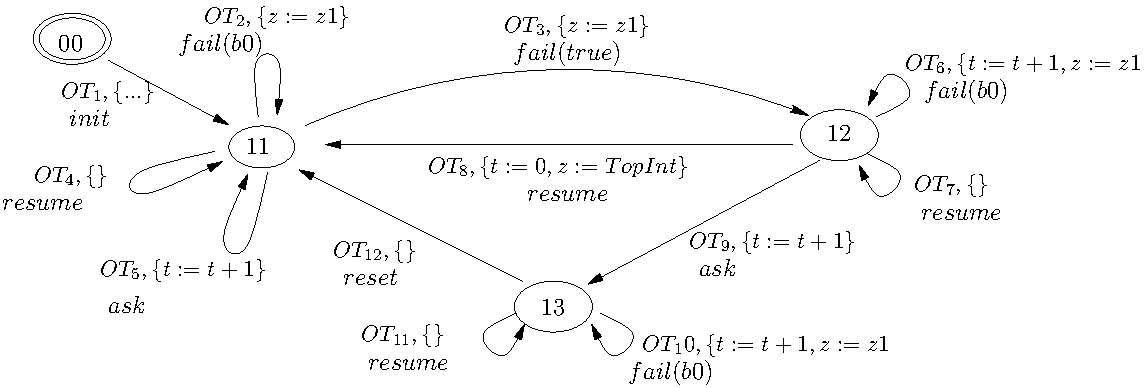
\includegraphics[width=\columnwidth]{TimerOADetailed}
  \caption{The open Automaton of the Failure Monitor Architecture}
  \label{schema:ArchFailure:BIP}
\end{figure}


$  OT_1  = \openrule
{\emptyset, \{t:=0, z:=TopInt, zone:=[minZone,maxZone]\} }
{\ostate{00} \OTarrow{\underline{\alpha_4}} \ostate{11}}
$
\medskip
    
$  OT_2  = \openrule
{\{B\mapsto fail(b0)\},\\
  t<GetMax(z) \land b1=false \land b1=>b0 \land z1= (z \cap (b1?zone;TopInt)+t),
  \{z:=z1\} }
{\ostate{11} \OTarrow{\underline{\alpha_0}} \ostate{11}}
$
\medskip
  
  $  OT_3  = \openrule
  {\{B\mapsto fail(b0)\},\\
    t<GetMax(z) \land b1=true \land b1=>b0 \land z1= (z \cap (b1?zone;TopInt)+t),
    \{z:=z1\} }
  {\ostate{11} \OTarrow{\underline{\alpha_0}} \ostate{12}}
  $
  \medskip

  $  OT_4  = \openrule
  {\{B\mapsto resume\},
    b1=false \land b2=false \land b1=b2
    \{\}  }
  {\ostate{11} \OTarrow{\underline{\alpha_1}} \ostate{11}}
  $
  \medskip
  
  $  OT_5  = \openrule
  {\{E\mapsto ask\},
    t \in z,
    \{t:=t+1\}  }
  {\ostate{11} \OTarrow{\underline{\alpha_2}} \ostate{11}}
  $
  \medskip

  $  OT_7  = \openrule
  {\{B\mapsto resume\},
    b1=false \land b2=false \land b1=b2,
    \{\} }
  {\ostate{12} \OTarrow{\underline{\alpha_1}} \ostate{12}}
  $
  \medskip

  $  OT_8  = \openrule
  {\{B\mapsto resume\},
    b1=true \land b2=true \land b1=b2, 
    \{t:=0, z:=TopInt\} }
  {\ostate{12} \OTarrow{\underline{\alpha_1}} \ostate{11}}
  $
  \medskip

  $  OT_9  = \openrule
  {\{E\mapsto ask\},
    t \in z,
    \{t:=t+1\} }
  {\ostate{12} \OTarrow{\underline{\alpha_2}} \ostate{13}}
  $
  \medskip

  $  OT_{10}  = \openrule
  {\{B\mapsto fail(b0)\},\\
    t<GetMax(z) \land b1=false \land b1=>b0 \land z1=(z \cap (b1?zone;TopInt)+t),
    \{t:=t+1, z:=z1\} }
  {\ostate{13} \OTarrow{\underline{\alpha_0}} \ostate{13}}
  $
  \medskip

  $  OT_{11}  = \openrule
  {\{B\mapsto resume\},
    b1=false \land b2=false \land b1=b2,
    \{\} }
  {\ostate{13} \OTarrow{\underline{\alpha_1}} \ostate{13}}
  $
  \medskip

  $  OT_{12}  = \openrule
  {\{E\mapsto reset\},
    true,
    \{\} }
  {\ostate{13} \OTarrow{\underline{\alpha_3}} \ostate{11}}
  $

\end{document}
